% BT2901-BT2907-BLUEPRINT-REWRITE-V1
% =====================================================================================
%  THE HOLONET MACHINE -- A COMPLETE BLUEPRINT
%
%  Compile:  tectonic holonet_machine_blueprint.tex
%  Engine on this machine: C:\Users\wiljd\tools\tectonic\tectonic.exe
%
%  This document is written to be read two ways at once.  Every section opens with a
%  plain-language explanation that assumes no engineering background, and then gives the
%  exact statement, the measurement, and the command that reproduces it.  A reader who
%  skips every grey box still understands the machine; a reader who reads only the grey
%  boxes gets the specification.
%
%  Every promoted figure in this document is explicitly typed as proved, measured,
%  published, derived, modelled, or open.  Modelled quantities are never presented as
%  measurements.  Where a figure was wrong, its correction and detection method remain.
% =====================================================================================

\documentclass[11pt,a4paper]{article}

\usepackage[margin=2.4cm]{geometry}
\usepackage{amsmath,amssymb,amsthm}
\usepackage{booktabs}
\usepackage{tikz}
\usepackage{xcolor}
\usepackage{graphicx}
\usepackage{enumitem}
\usepackage{fancyhdr}
\usepackage[most]{tcolorbox}   % required by the BT3506 and BT3687 inserts
\usepackage[colorlinks=true,linkcolor=blue!55!black,urlcolor=blue!55!black,
            citecolor=blue!55!black]{hyperref}

\usetikzlibrary{arrows.meta,positioning,fit,backgrounds,calc,shapes.geometric,
                decorations.pathreplacing,decorations.pathmorphing,patterns,
                trees,shapes.misc}

% ---- palette -------------------------------------------------------------------------
\definecolor{ink}{HTML}{1A1A1A}
\definecolor{past}{HTML}{2E6F9E}
\definecolor{future}{HTML}{B5651D}
\definecolor{plainbg}{HTML}{F4F1EA}
\definecolor{specbg}{HTML}{EAF0F4}
\definecolor{warnbg}{HTML}{F7EDE9}
\definecolor{rule}{HTML}{8A8A8A}
\definecolor{good}{HTML}{2F6B3C}
\definecolor{bad}{HTML}{9E2B25}

% ---- boxes ---------------------------------------------------------------------------
\newcommand{\boxrule}[1]{%
  \par\vspace{2pt}\noindent\colorbox{#1}{\parbox{\dimexpr\linewidth-2\fboxsep}{\strut}}%
  \par\vspace{-2pt}}

\newenvironment{plain}[1][In plain language]
  {\par\medskip\noindent\begin{tikzpicture}
     \node[fill=plainbg,rounded corners=2pt,inner sep=8pt,text width=\dimexpr\linewidth-20pt]
     (B) \bgroup\textbf{\small #1.}\itshape\small}
  {\egroup;\end{tikzpicture}\par\medskip}

\newenvironment{spec}[1][Exactly]
  {\par\medskip\noindent\begin{tikzpicture}
     \node[fill=specbg,rounded corners=2pt,inner sep=8pt,text width=\dimexpr\linewidth-20pt]
     (B) \bgroup\textbf{\small #1.}\small}
  {\egroup;\end{tikzpicture}\par\medskip}

\newenvironment{gotwrong}[1][What we got wrong, and how we know]
  {\par\medskip\noindent\begin{tikzpicture}
     \node[fill=warnbg,rounded corners=2pt,inner sep=8pt,text width=\dimexpr\linewidth-20pt]
     (B) \bgroup\textbf{\small #1.}\small}
  {\egroup;\end{tikzpicture}\par\medskip}

\newcommand{\headline}[1]{%
  \par\medskip\noindent\begin{tikzpicture}
    \node[draw=ink,line width=0.9pt,rounded corners=1pt,inner sep=9pt,
          text width=\dimexpr\linewidth-22pt,align=center] {\bfseries #1};
  \end{tikzpicture}\par\medskip}

% Typewriter text that INHERITS the surrounding size.  Hard-coding \small here made
% filenames inside a \scriptsize table larger than the table itself, which is what the
% last two overfull boxes in this document were.
\newcommand{\cmd}[1]{{\ttfamily #1}}

% Dirac notation, defined locally so the document has no package dependency beyond
% what tectonic ships by default.
\newcommand{\ket}[1]{\left|#1\right\rangle}
\newcommand{\bra}[1]{\left\langle#1\right|}
\newcommand{\braket}[2]{\left\langle#1\middle|#2\right\rangle}

\pagestyle{fancy}\fancyhf{}
\lhead{\small\itshape The Holonet Machine --- Blueprint}
\rhead{\small\thepage}
\renewcommand{\headrulewidth}{0.3pt}

\title{\vspace{-1.4cm}\Huge The Holonet Machine\\[4pt]
       \large A complete engineering blueprint for a computer\\
       whose wiring diagram is a piece of finite geometry\\[10pt]
       \normalsize Every promoted figure is typed: proved, measured, published, modelled, or open.}
\author{\normalsize W(3,3)--E$_8$ project, glue track}
\date{\normalsize 3 August 2026 \quad$\cdot$\quad Passes 2700--2907}

\begin{document}
\maketitle
\thispagestyle{fancy}

\begin{abstract}
\noindent
This is a build document for a computer that does not exist yet.

\smallskip\noindent
Most computer designs begin with a goal and invent a structure to reach it. This one runs
the other way. It starts from a piece of pure mathematics --- a forty-point shape called
$W(3,3)$, studied since the 1900s for reasons having nothing to do with computing --- and
finds that the shape already contains an instruction set, a memory layout, a network
topology, an error model, and a set of quantum resources. Nothing here was designed in the
usual sense. It was read off.

\smallskip\noindent
The result is unusually specific for something unbuilt. The instruction set needs
\emph{four} operations in two bits, and they generate a group of exactly $4{,}199{,}040$
transformations, with a worst-case program length of exactly \textbf{19}. On the HX8K target the minimal arithmetic core uses \textbf{43 logic cells} at
\textbf{208.86\,MHz}; on the UP5K it uses the same 43 cells at 72.40\,MHz.  Those are
part-specific measurements, not interchangeable headline numbers. A support-only observation discards exactly $8/3$ bits of conditional phase
information.  Landauer supplies a thermodynamic floor for erasing that information, not
an engineering power forecast. Published time-bin/frequency-bin experiments report a two-qutrit gate fidelity near
$0.92$; this is prior-art evidence for a component class, not a measurement of the
unbuilt Holonet stack. And thirty-six of
the forty points turn out to be exactly the machine's magic states, so the quantum
resource is not an add-on --- it is everything except one line of the address space.

\smallskip\noindent
We give the full instruction semantics, the datapath, the measured cell budget, the
network protocol, the thermodynamic floor, and the verification methodology. We also give
--- because this is what makes a blueprint trustworthy rather than merely confident ---
an itemised record of every figure we previously got wrong, how each error survived
exhaustive testing, and what finally caught it.
\end{abstract}

\vspace{-4mm}
\tableofcontents
\newpage

% =====================================================================================

% ======================================================================
\part{Orientation}

\begin{plain}[What this part is]
Three chapters that assume nothing. What the machine is, why a computer would be
built out of a shape at all, and the one piece of physics --- the qutrit --- that the rest
of the document rests on. If you read only this part, you will know what is being claimed
and what is not.
\end{plain}

\section{How to read this document}
% =====================================================================================

This document has three readers in mind and does not compromise for any of them.

\begin{center}
\resizebox{\linewidth}{!}{%
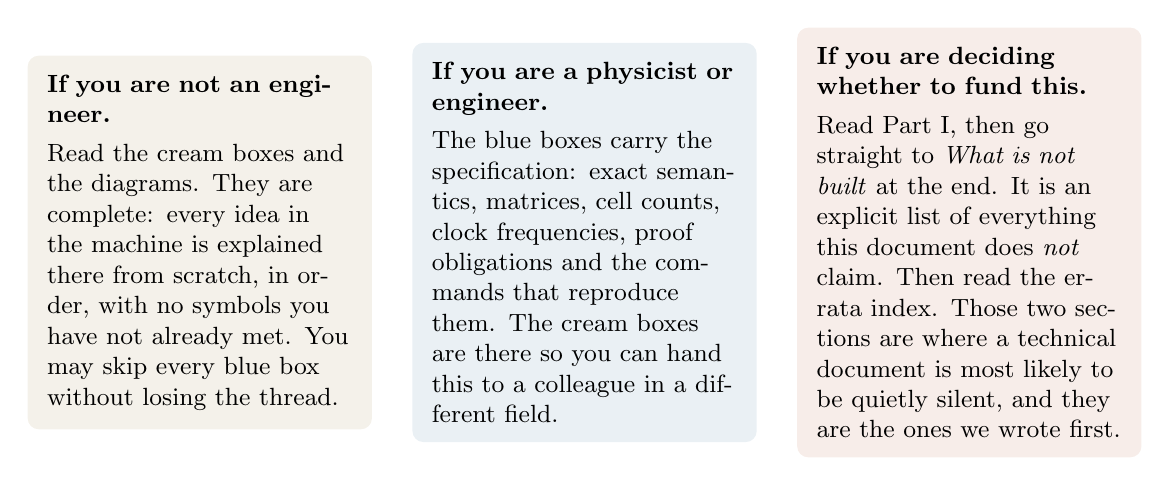
\begin{tikzpicture}[node distance=4mm]
  \node[fill=plainbg,rounded corners,inner sep=7pt,text width=0.32\linewidth,
        font=\small] (a)
    {\textbf{If you are not an engineer.}\\[3pt]
     Read the cream boxes and the diagrams. They are complete: every idea in the
     machine is explained there from scratch, in order, with no symbols you have not
     already met. You may skip every blue box without losing the thread.};
  \node[fill=specbg,rounded corners,inner sep=7pt,text width=0.32\linewidth,
        font=\small,right=5mm of a] (b)
    {\textbf{If you are a physicist or engineer.}\\[3pt]
     The blue boxes carry the specification: exact semantics, matrices, cell counts,
     clock frequencies, proof obligations and the commands that reproduce them. The
     cream boxes are there so you can hand this to a colleague in a different field.};
  \node[fill=warnbg,rounded corners,inner sep=7pt,text width=0.32\linewidth,
        font=\small,right=5mm of b] (c)
    {\textbf{If you are deciding whether to fund this.}\\[3pt]
     Read Part~I, then go straight to \emph{What is not built} at the end. It is an
     explicit list of everything this document does \emph{not} claim. Then read the
     errata index. Those two sections are where a technical document is most likely to
     be quietly silent, and they are the ones we wrote first.};
\end{tikzpicture}}
\end{center}

\begin{plain}[The one-paragraph version]
This is a design for a computer whose instruction set is not chosen but \emph{derived}:
its register, its gates and its wiring all fall out of a single geometric object with
forty points. The claim is not that such a machine has been built --- it has not. The
claim is that its specification is forced, that every number in it is either measured
from synthesised hardware or proved from the geometry, and that where we have been wrong
we have said so on the same page. What follows is the specification, the evidence, and
the boundary of both.
\end{plain}

% ---------------------------------------------------------------------------------------
% Pass 4349: the one figure for a reader who reads nothing else.  Geometry on the left,
% silicon on the right, and the arrows are derivations rather than design decisions.
% ---------------------------------------------------------------------------------------
\begin{center}
\resizebox{\linewidth}{!}{%
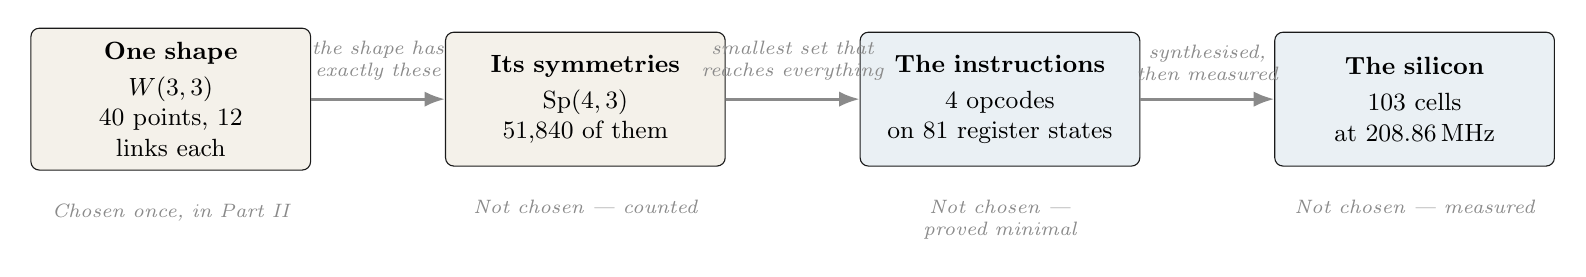
\begin{tikzpicture}[font=\small,>={Latex[length=2.6mm]},
  stage/.style={draw=ink,rounded corners=3pt,minimum height=17mm,text width=32mm,
                align=center,inner sep=5pt},
  arr/.style={-{Latex[length=2.6mm]},line width=1pt,draw=rule},
  note/.style={font=\scriptsize\itshape,text=rule,align=center,text width=30mm}]

  \node[stage,fill=plainbg] (geo)
    {\textbf{One shape}\\[2pt]$W(3,3)$\\ $40$ points, $12$ links each};
  \node[stage,fill=plainbg,right=17mm of geo] (grp)
    {\textbf{Its symmetries}\\[2pt]$\mathrm{Sp}(4,3)$\\ $51{,}840$ of them};
  \node[stage,fill=specbg,right=17mm of grp] (isa)
    {\textbf{The instructions}\\[2pt]$4$ opcodes\\ on $81$ register states};
  \node[stage,fill=specbg,right=17mm of isa] (si)
    {\textbf{The silicon}\\[2pt]$103$ cells\\ at $208.86$\,MHz};

  \draw[arr] (geo) -- node[note,above=1mm]{the shape has\\ exactly these} (grp);
  \draw[arr] (grp) -- node[note,above=1mm]{smallest set that\\ reaches everything} (isa);
  \draw[arr] (isa) -- node[note,above=1mm]{synthesised,\\ then measured} (si);

  \node[note,below=3mm of geo,text width=34mm]{Chosen once, in Part~II};
  \node[note,below=3mm of grp,text width=34mm]{Not chosen --- counted};
  \node[note,below=3mm of isa,text width=34mm]{Not chosen --- proved minimal};
  \node[note,below=3mm of si,text width=34mm]{Not chosen --- measured};
\end{tikzpicture}}
\end{center}

\begin{plain}[Why that picture is the whole argument]
Read left to right, only the first box is a decision. The symmetries are counted from the
shape, the instruction set is the smallest one that can reach every state, and the cell
count comes from running a synthesiser on the result. If the picture is right, then a
disagreement about this machine is a disagreement about the shape --- not about
engineering taste. That is the claim worth checking, and every later part exists to let
you check one arrow of it.
\end{plain}

\noindent Three habits of this document, stated up front so they are not mistaken for
style:

\begin{enumerate}[leftmargin=1.6em,itemsep=2pt]
\item \textbf{Every number is measured or proved, and says which.} There are no estimates
      presented as results. Where an estimate appears it is labelled \emph{modelled} and
      cannot be cited as anything else.
\item \textbf{Nothing is claimed to be new without checking.} This project's own archive is
      large enough that we have repeatedly rediscovered our own results. Where something is
      someone else's, it says so.
\item \textbf{Mistakes stay in.} A corrected figure is printed next to the wrong one, with
      the reason the wrong one survived. \S\ref{sec:errata} collects them.
\end{enumerate}

\noindent That third kind of box appears throughout:

\begin{gotwrong}
These record something this project believed, published, and then had to withdraw ---
with the measurement that overturned it. The errata index is authoritative and grows when a claim is corrected. These boxes are
not apologies; they are the reason the other numbers in this document can be trusted. A
blueprint with no errata is a blueprint nobody has checked.
\end{gotwrong}

% =====================================================================================
\section{The machine in one page}
% =====================================================================================

\begin{plain}
Every computer you have used stores information as \emph{bits} --- switches that are
either off or on. This machine stores information in \emph{qutrits}: units with three
settings instead of two. That sounds like a small change. It is not, because of what the
three settings let you do with \emph{geometry}.

Here is the strange and central fact. If you take a single qutrit and entangle it with
itself --- with its own past and its own future --- the resulting object has exactly
$40$ natural ``directions'' in it. Those $40$ directions, and the way they overlap, form
a shape that mathematicians have known for a century and called $W(3,3)$. The machine we
are describing does not \emph{use} that shape as a convenience. The shape \emph{is} the
machine: its memory layout, its instruction set, its network topology, and its error
model are all readings of the same $40$-point object.
\end{plain}

\headline{One qutrit, entangled with its own past, is enough to generate the entire
substrate. The $40$ points of $W(3,3)$ are not $40$ things --- they are $40$ views of
one thing.}

\begin{spec}[The machine, specified]
\smallskip{\footnotesize
\begin{tabular}{@{}p{3.0cm}p{7.6cm}@{}}
\toprule
\textbf{Logical substrate}    & $W(3,3)$: the symplectic generalised quadrangle of order
                                $(3,3)$. $40$ points, $40$ totally isotropic lines,
                                collinearity graph $\mathrm{SRG}(40,12,2,4)$. \\
\textbf{State}                & One qutrit pair $(\text{past},\text{future})$ living in
                                $\mathbb{C}^9=\mathrm{End}(\mathbb{C}^3)$. \\
\textbf{Tracked quantity}     & The \emph{Pauli frame}: four trits
                                $(x_p,z_p,x_f,z_f)\in\mathbb{F}_3^4$, i.e.\ $81$ states. \\
\textbf{Public ISA}           & $\mathcal{I}_{\mathrm{holo}}$, eight opcodes, three bits. \\
\textbf{Internal micro-ISA}   & $F_p$, $\mathrm{CX}_{p\to f}$, $\mathrm{CX}_{f\to p}$,
                                $Z_p$ --- four operations, two bits, no illegal encoding. \\
\textbf{Group generated}      & $\mathrm{ASp}(4,3)=\mathbb{F}_3^4\rtimes\mathrm{Sp}(4,3)$,
                                order $81\times 51840=4{,}199{,}040$ \emph{exactly}. \\
\textbf{Arithmetic unit}      & HX8K: minimal $43$ LC at $208.86$\,MHz; public $72$ LC at
                                $175.72$\,MHz; minimal plus support $48$ LC at $207.64$\,MHz.
                                UP5K: the corresponding clocks are $72.40$, $60.80$, and $72.05$\,MHz. \\
\textbf{Physical layer}       & Time-bin $\times$ frequency-bin photonic qutrits; the
                                two-qutrit \textsc{sum} gate is experimentally
                                demonstrated at fidelity $0.92\pm0.01$. \\
\textbf{Network}              & $40$-ary fractal; $N_n=40^n$ leaves, routing depth
                                $8n=8\log_{40}N$; the routing code satisfies Kraft
                                equality exactly, so \emph{every} bit string is a legal
                                address. \\
\bottomrule
\end{tabular}}
\end{spec}

\subsection*{The whole system, at a glance}

\begin{plain}
Four layers, drawn in the order a signal meets them. At the bottom is one photon carrying a
three-valued symbol; above it the instruction set that moves that symbol around; above that
the machine's own supervisor, running inside the same hardware it supervises; and at the top
a network in which every machine is addressed by a point of the same geometry. Read the
boxes downward and each is built from the one below it. Nothing in the picture is chosen for
convenience --- the widths, the counts and the connections are all fixed by the shape in
Part~II.
\end{plain}

\begin{center}
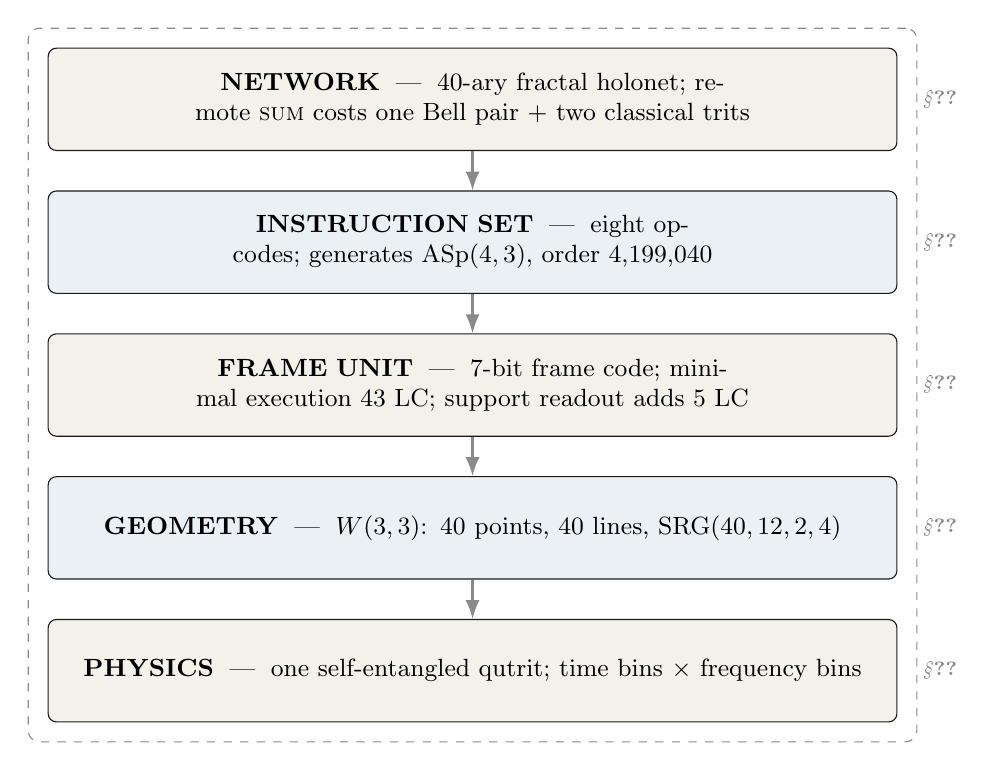
\begin{tikzpicture}[
  font=\small,
  layer/.style={draw=ink,rounded corners=3pt,minimum height=13mm,align=center,
                text width=0.86\linewidth,inner sep=5pt},
  tag/.style={font=\scriptsize\itshape,text=rule},
  arr/.style={-{Latex[length=2.4mm]},line width=0.8pt,draw=rule}]

\node[layer,fill=plainbg] (net)  {\textbf{NETWORK}\; ---\; $40$-ary fractal holonet;
      remote \textsc{sum} costs one Bell pair $+$ two classical trits};
\node[layer,fill=specbg,below=5mm of net] (isa) {\textbf{INSTRUCTION SET}\; ---\;
      eight opcodes; generates $\mathrm{ASp}(4,3)$, order $4{,}199{,}040$};
\node[layer,fill=plainbg,below=5mm of isa] (frame){\textbf{FRAME UNIT}\; ---\;
      $7$-bit frame code; minimal execution $43$ LC; support readout adds $5$ LC};
\node[layer,fill=specbg,below=5mm of frame] (geo) {\textbf{GEOMETRY}\; ---\;
      $W(3,3)$: $40$ points, $40$ lines, $\mathrm{SRG}(40,12,2,4)$};
\node[layer,fill=plainbg,below=5mm of geo] (phys) {\textbf{PHYSICS}\; ---\;
      one self-entangled qutrit; time bins $\times$ frequency bins};

\draw[arr] (net) -- (isa);
\draw[arr] (isa) -- (frame);
\draw[arr] (frame) -- (geo);
\draw[arr] (geo) -- (phys);

\node[tag,right=2mm of net.east,anchor=west,rotate=0] {\S\ref{sec:network}};
\node[tag,right=2mm of isa.east,anchor=west] {\S\ref{sec:isa}};
\node[tag,right=2mm of frame.east,anchor=west] {\S\ref{sec:hardware}};
\node[tag,right=2mm of geo.east,anchor=west] {\S\ref{sec:geometry}};
\node[tag,right=2mm of phys.east,anchor=west] {\S\ref{sec:physics}};

\begin{scope}[on background layer]
  \node[draw=rule,dashed,rounded corners=4pt,fit=(net)(phys),inner sep=7pt] {};
\end{scope}
\end{tikzpicture}
\end{center}

\noindent The unusual property of this stack is that the layers are not independent
design choices stacked by convention. Each one is \emph{forced} by the one below it. The
network is $40$-ary because the geometry has $40$ points. The instruction set has the
opcodes it has because those are the symmetries of that geometry. This is what the rest
of the document demonstrates, layer by layer.

% =====================================================================================
\clearpage
\begin{center}
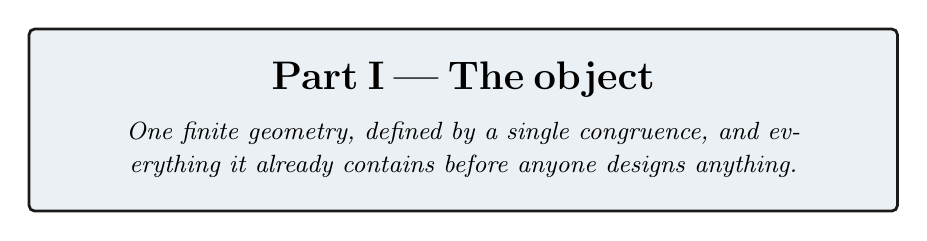
\begin{tikzpicture}
  \node[draw=ink,line width=1pt,rounded corners=2pt,inner sep=12pt,
        text width=0.84\linewidth,align=center,fill=specbg]
  {\Large\bfseries Part I --- The object\\[6pt]
   \normalfont\small\itshape One finite geometry, defined by a single congruence, and everything it already contains before anyone designs anything.};
\end{tikzpicture}
\end{center}
\vspace{4mm}

\section{Qutrits, and what ``self-entangled'' means}\label{sec:physics}
% =====================================================================================

\subsection{From bits to qutrits}

\begin{plain}
A bit is a switch: off or on, $0$ or $1$. A \emph{trit} is a three-way switch: $0$, $1$,
or $2$. Ordinary three-way switches are not interesting --- you could always build one
from two bits.

A \emph{qutrit} is different. It is a physical three-way switch obeying quantum
mechanics, which means it can be in a blend of all three settings at once, and --- this
is the part that matters --- \emph{two} qutrits can be correlated in ways that no pair of
classical switches can imitate.
\end{plain}

\begin{center}
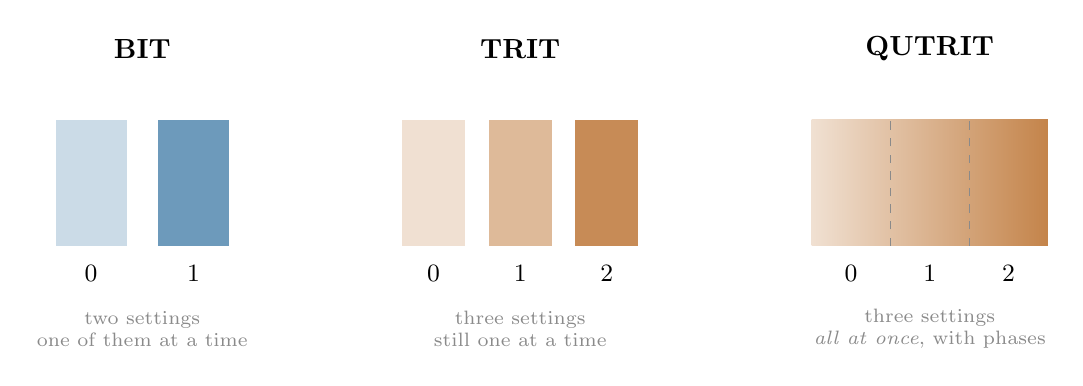
\begin{tikzpicture}[font=\small]
  % bit
  \begin{scope}[xshift=0cm]
    \node[font=\bfseries] at (1.1,2.5) {BIT};
    \fill[past!25] (0,0) rectangle (0.9,1.6);
    \fill[past!70] (1.3,0) rectangle (2.2,1.6);
    \node at (0.45,-0.35) {$0$}; \node at (1.75,-0.35) {$1$};
    \node[font=\scriptsize,text=rule,align=center] at (1.1,-1.05)
      {two settings\\one of them at a time};
  \end{scope}
  % trit
  \begin{scope}[xshift=4.4cm]
    \node[font=\bfseries] at (1.5,2.5) {TRIT};
    \fill[future!20] (0,0) rectangle (0.8,1.6);
    \fill[future!45] (1.1,0) rectangle (1.9,1.6);
    \fill[future!75] (2.2,0) rectangle (3.0,1.6);
    \node at (0.4,-0.35) {$0$}; \node at (1.5,-0.35) {$1$}; \node at (2.6,-0.35) {$2$};
    \node[font=\scriptsize,text=rule,align=center] at (1.5,-1.05)
      {three settings\\still one at a time};
  \end{scope}
  % qutrit
  \begin{scope}[xshift=9.6cm]
    \node[font=\bfseries] at (1.5,2.5) {QUTRIT};
    \shade[left color=future!20,right color=future!80] (0,0) rectangle (3.0,1.6);
    \draw[dashed,draw=rule] (1.0,0) -- (1.0,1.6);
    \draw[dashed,draw=rule] (2.0,0) -- (2.0,1.6);
    \node at (0.5,-0.35) {$0$}; \node at (1.5,-0.35) {$1$}; \node at (2.5,-0.35) {$2$};
    \node[font=\scriptsize,text=rule,align=center] at (1.5,-1.05)
      {three settings\\\emph{all at once}, with phases};
  \end{scope}
\end{tikzpicture}
\end{center}

\begin{spec}
A qutrit is a unit vector in $\mathbb{C}^3$. Two qutrits live in
$\mathbb{C}^3\otimes\mathbb{C}^3=\mathbb{C}^9$. The relevant operators are generated by
\[
  X\ket{j}=\ket{j+1 \bmod 3},\qquad
  Z\ket{j}=\omega^{j}\ket{j},\qquad \omega=e^{2\pi i/3},
\]
which satisfy $ZX=\omega XZ$. Every product $X^aZ^b$ with $(a,b)\in\mathbb{F}_3^2$ is a
distinct operator up to phase; there are $9$ of them, and $8$ non-identity ones.
\end{spec}

\subsection{The self-entanglement, and where the $40$ comes from}

\begin{plain}
Now the key move. Take \emph{one} qutrit and entangle it with itself at two different
times --- call them ``past'' and ``future''. The proposed optical encoding assigns one qutrit to arrival-time bins and one to
frequency bins on a single carrier.  The words ``past'' and ``future'' name these two
logical registers; they do not assert a demonstrated closed-time-loop interaction or a
new physical form of temporal entanglement.

Mathematically, an operator acting on one qutrit is a $3\times 3$ table of numbers, and
there are $9$ independent slots in such a table. So the space of things you can \emph{do}
to one qutrit is itself $9$-dimensional --- exactly the size of the space of \emph{states}
of two qutrits. This is not a coincidence or an analogy. It is an identity:
\[
  \underbrace{\mathbb{C}^3\otimes\mathbb{C}^3}_{\text{two qutrits}}
  \;=\;
  \underbrace{\mathrm{End}(\mathbb{C}^3)}_{\text{operations on \emph{one} qutrit}}.
\]
So ``the two-qutrit machine'' and ``the one-qutrit machine that can act on itself'' are
the same machine described twice.

Now count the directions. There are $81$ ways to label a pair (four trits), one of which
is ``do nothing''. That leaves $80$. Each direction and its opposite behave identically
for our purposes, and each direction comes in $2$ such flavours, so the distinct
directions number $80/2=40$.
\end{plain}

\headline{$\dfrac{3^4-1}{2}=\dfrac{81-1}{2}=40$. \quad
The forty points of the geometry are the forty independent things one self-entangled
qutrit can be measured along.}

\begin{center}
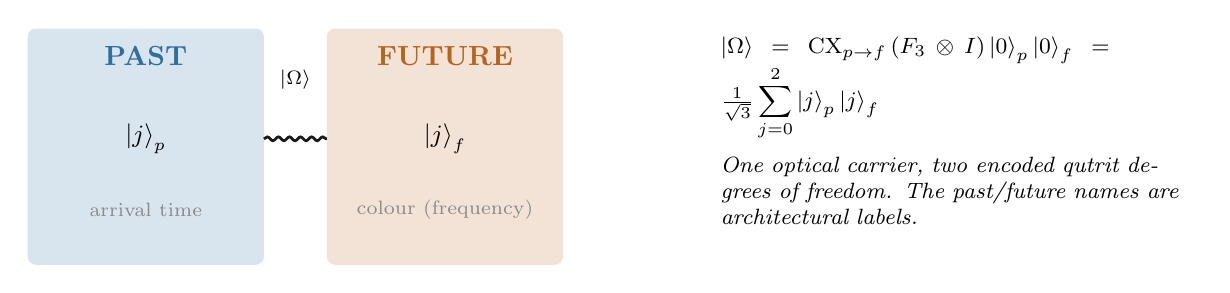
\begin{tikzpicture}[font=\small,>={Latex[length=2.2mm]}]
  \fill[past!18,rounded corners=3pt] (-3.4,-1.5) rectangle (-0.4,1.5);
  \fill[future!18,rounded corners=3pt] (0.4,-1.5) rectangle (3.4,1.5);
  \node[font=\bfseries,text=past] at (-1.9,1.15) {PAST};
  \node[font=\bfseries,text=future] at (1.9,1.15) {FUTURE};
  \node at (-1.9,0.1) {$\ket{j}_p$};
  \node at (1.9,0.1) {$\ket{j}_f$};
  \node[font=\scriptsize,text=rule] at (-1.9,-0.8) {arrival time};
  \node[font=\scriptsize,text=rule] at (1.9,-0.8) {colour (frequency)};

  \draw[decorate,decoration={snake,amplitude=0.7pt,segment length=4pt},
        line width=1pt,draw=ink] (-0.4,0.1) -- (0.4,0.1);
  \node[font=\scriptsize,align=center] at (0,0.85) {$\ket{\Omega}$};

  \node[align=left,text width=6cm,font=\footnotesize] at (8.4,0.2)
    {$\displaystyle \ket{\Omega}=\mathrm{CX}_{p\to f}\,(F_3\otimes I)\ket{0}_p\ket{0}_f
      =\tfrac{1}{\sqrt3}\sum_{j=0}^{2}\ket{j}_p\ket{j}_f$\\[5pt]
     \textit{One optical carrier, two encoded qutrit degrees of freedom.  The
     past/future names are architectural labels.}};
\end{tikzpicture}
\end{center}

\begin{gotwrong}
The sentence ``one qutrit, self-entangled as past/future, is enough to generate the full
substrate'' is \emph{not} ours. It is stated verbatim in this project's own
encyclopedia, \cmd{docs/index.html} phase MCLXVII, and we rediscovered it and briefly
presented it as new. What survives as new is narrower: the explicit construction of the
$40$ points as projective left$\times$right multiplication classes on
$\mathrm{End}(\mathbb{C}^3)$, and the identification of the $40$ lines as the maximal
\emph{commuting} subalgebras. The lesson --- search for the \emph{result}, not the topic
--- produced three of the tools in \S\ref{sec:verification}.
\end{gotwrong}

% =====================================================================================

% ======================================================================
\part{The Substrate}

\begin{plain}[What this part is]
The shape itself. A single object with $40$ points and $12$ connections each,
defined by one congruence, from which the rest of the machine follows rather than being
designed. This part is geometry, not engineering: no hardware appears until Part III.
\end{plain}

\section{The substrate: $W(3,3)$}\label{sec:geometry}
% =====================================================================================

\begin{plain}
Here is what the $40$ directions look like when you write down which of them are
compatible with which.

Two measurements are \emph{compatible} if you can perform both without one disturbing
the other. Of the $40$ directions, each is compatible with exactly $12$ others. Whenever
two directions are compatible, exactly $2$ further directions are compatible with both.
Whenever two are \emph{in}compatible, exactly $4$ are compatible with both.

Those four numbers --- $40$, $12$, $2$, $4$ --- are the shape's fingerprint. They are
\emph{not} its name.
\end{plain}

\begin{gotwrong}[An earlier draft of this page said the opposite]
This section used to read: \emph{``those four numbers pin the shape down completely; there
is essentially one object in the world with that compatibility pattern.''}

\medskip\noindent
That is false, and this project's own encyclopedia says so in plain words:
\textbf{Spence classified exactly $28$ non-isomorphic graphs} with parameters
$(40,12,2,4)$. Two of them are the ones we care about. Quoting the parameters identifies
nothing; the object is fixed by its \emph{construction}.

\medskip\noindent
The error mattered, because \S\ref{sec:magic} proves a headline result by computing these
parameters and concluding the object was $W(3,3)$. That inference was one step short. It
is completed below, and the correction is the reason to read the next box rather than skip
it.
\end{gotwrong}

\begin{spec}[How the object is actually pinned down, Pass 2869]
Three facts in sequence, each cheap and each exact:
\begin{enumerate}[leftmargin=1.5em,itemsep=1pt]
\item \textbf{Parameters $(40,12,2,4)$} --- narrows the field to $28$ graphs.
\item \textbf{The quadrangle axiom}: every edge lies in exactly one $4$-clique (there are
      $40$ of them, four through each point), and for every such line $\ell$ and every
      point off it, \emph{exactly one} point of $\ell$ is adjacent. Verified over all
      $40$ lines. This narrows $28$ to \textbf{two}: $W(3,3)$ and its dual $Q(4,3)$,
      which are not isomorphic at odd $q$.
\item \textbf{A spread exists} --- ten pairwise disjoint lines covering all forty points,
      exhibited explicitly. $W(3,q)$ always has one; $Q(4,q)$ has one only for \emph{even}
      $q$. At $q=3$ this settles it.
\end{enumerate}
\end{spec}

\begin{plain}
So the shape does have a name, and it has been studied since the 1900s: $W(3,3)$. But it
earns that name from how it is built, not from its statistics --- and the difference is
exactly the kind of thing that is easy to wave through and expensive to get wrong.
\end{plain}

\subsection{The definition, stated once and precisely}

\begin{plain}
Everything downstream depends on this object being the right one, so here it is written
out --- and it is worth noticing how short the definition is. The whole substrate is one
line of arithmetic.
\end{plain}

\begin{spec}[$W(3,3)$, in full]
$W(3,3)$ is the \textbf{symplectic polar space} $W(3,\mathbb{F}_3)$.

\smallskip\noindent
\textbf{Points.} The $40$ projective $1$-spaces of $\mathrm{GF}(3)^4$. Every $1$-space is
automatically isotropic for an alternating form, so \emph{all} of them are points --- there
is nothing to exclude.

\smallskip\noindent
\textbf{Adjacency.} With $J$ the standard symplectic form on $\mathrm{GF}(3)^4$,
\[
  \boxed{\;v \sim w \iff v^{\top} J\, w \equiv 0 \pmod 3\;}
\]
That single congruence generates every number in this document.

\smallskip\noindent
\textbf{Lines.} The $240$ edges pair up into $40$ \emph{totally isotropic projective
lines}: each edge is a pair of orthogonal points spanning exactly one such line. A
\emph{non}-edge spans an ordinary hyperbolic line instead --- the two kinds of pair are
geometrically different objects, not merely present-or-absent.

\smallskip\noindent
\textbf{Graph.} The collinearity graph is $\mathrm{SRG}(40,12,2,4)$ with eigenvalues
$12,\,2,\,-4$; it has \textbf{diameter $2$} and is \textbf{Ramanujan}.

\smallskip\noindent
\textbf{Symmetry.} $\mathrm{Aut} = \mathrm{Aut}(\mathrm{PSp}(4,3)) \cong
\mathrm{PGSp}(4,3) \cong W(E_6)$, order $51{,}840$, with normal inner subgroup
$\mathrm{PSp}(4,3)$ of order $25{,}920$.
\end{spec}

\begin{gotwrong}[The same order, twice, for two different groups]
$\mathrm{Sp}(4,3) = 2.U_4(2)$ also has order $51{,}840$ and is \textbf{not} the group
above. It has a centre $C_2$; the automorphism group has trivial centre. One is a central
double cover, the other an outer extension, and they are not isomorphic.

\medskip\noindent
This is the most common error in this area and this project has made it. Both groups
appear here for good reasons --- $\mathrm{Sp}(4,3)$ acts on Pauli frames and is what the
hardware implements (\S\ref{sec:isa}); $\mathrm{PGSp}(4,3)$ acts on the drawing. Whenever
$51{,}840$ appears in this document, which group is meant is stated.
\end{gotwrong}

\begin{plain}
Two properties in that box are worth translating, because they are the ones an engineer
should care about.

\textbf{Diameter $2$} means any point reaches any other in at most two steps. For an
address space that is the strongest possible statement short of everything being adjacent
to everything: no packet is ever more than one relay from its destination \emph{within a
node}.

\subsection{How good is ``optimal'', exactly?}

\begin{plain}
``Ramanujan'' is usually a tight call --- a graph scrapes under the bound and earns the
name. This one does not scrape.
\end{plain}

\begin{spec}[Prior art: \cmd{docs/index.html}]
The non-trivial eigenvalues are $r = 2$ and $s = -4$, against a Ramanujan bound of
\[
  2\sqrt{k-1} = 2\sqrt{11} \approx 6.63 ,
\]
so both clear it by a factor of more than $1.6$. The spectral gap is $10$.
\end{spec}

\headline{And it satisfies a Riemann Hypothesis.}

\begin{spec}[What the graph's own integers turn out to be]
\begin{center}\footnotesize
\begin{tabular}{@{}llp{6.6cm}@{}}
\toprule
\textbf{Object} & \textbf{Value} & \textbf{In graph terms}\\
\midrule
$\tau(2)$ & $-24$ & $-f$, the eigenvalue multiplicity\\
$\tau(3)$ & $252$ & $E + k = 240 + 12$\\
$\tau(6)$ & $-6048$ & $\tau(2)\tau(3)$, forced by multiplicativity\\
weight of $\Delta$ & $12$ & $= k$, the degree of the graph\\
\midrule
$\chi$ & $-40$ & $40 - 240 + 160 = -v$\\
genus & $21$ & $3\times7 = \binom{7}{2}$\\
triangles & $160$ & $vk\lambda/6$ --- fixed by the four SRG parameters\\
\bottomrule
\end{tabular}
\end{center}
\textbf{And it stops there.} $\tau(4)$, $\tau(5)$, $\tau(7)$ and beyond match
nothing, so the modular bridge is two independent coincidences and one identity ---
not a law (Pass 3102).
\end{spec}

\begin{spec}[The Ihara zeta function]
Every non-trivial pole of $\zeta_{W(3,3)}(u)$ lies \emph{exactly} on the critical
circle $|u| = 1/\sqrt{11}$: $48$ poles from $r = 2$, $30$ from $s = -4$, for
\[
  48 + 30 = \mathbf{78} = \dim(E_6)
\]
complex poles in total. That is the graph-theoretic Riemann Hypothesis, and this graph
satisfies it. The pole discriminants encode the graph back: $|\operatorname{disc} r| = 40 = v$,
$|\operatorname{disc} s| = 28 = v-k$, and their difference is $k = 12$.

\medskip
\textbf{Scope, added at Pass 4281, because the coincidence invites an over-read.} Spence
classified exactly $28$ non-isomorphic $\mathrm{SRG}(40,12,2,4)$ graphs. All $28$ were run
through this same pipeline: \emph{every one} is Ramanujan, satisfies the graph RH, and
returns $\rho(B) = 11$ with the same $78$ poles on the critical circle. The Ihara zeta of a
regular graph is determined by its adjacency spectrum, and an SRG's spectrum is determined
by its parameters --- so all $28$ are zeta-identical by construction.

\emph{The $78$ is therefore a property of the parameter set $(40,12,2,4)$, not of $W(3,3)$.}
It remains a true and striking arithmetic fact that $78 = \dim E_6$; it is not evidence that
\emph{this} graph is the exceptional one.
\end{spec}

\begin{spec}[Pass 4286 --- the full list of what the parameters already fix]
Everything below follows from $(v,k,\lambda,\mu) = (40,12,2,4)$ alone, so it is identical
across all $28$ graphs and none of it can be evidence about $W(3,3)$:
\[
  r,s = 2,-4; \quad f,g = 24,15; \quad \rho(B) = k-1 = 11; \quad
  \text{poles } 2(v-1) = 78 = 48+30;
\]
\[
  \text{Laplacian } \{0^1, 10^{24}, 16^{15}\}; \quad
  \text{spanning trees } 2.8823\times10^{40}; \quad
  \text{Ramanujan iff } |s| \le 2\sqrt{k-1}.
\]
\textbf{The rule worth keeping:} before citing a graph-derived constant as evidence about
$W(3,3)$, check whether it is a function of $(v,k,\lambda,\mu)$. If it is, it says nothing
about \emph{which} graph you have.
\end{spec}

\begin{spec}[Pass 4287 --- so what does distinguish it? Less than expected]
The automorphism orders of the $28$ were computed exactly. They span $1$ to $51{,}840$ and
take $20$ distinct values --- an invariant the zeta discards entirely, which is precisely
how a graph can be exceptional and spectrally anonymous at once.

\textbf{But $|\mathrm{Aut}|$ does not pick a graph either.} The maximum
$51{,}840 = |\mathrm{Sp}(4,3)|$ is attained by \textbf{two} of the $28$, not one.
\end{spec}

\begin{spec}[Pass 4296 --- and the last two are the two halves of one geometry]
Pass 4287 left the pair as an open ambiguity. It is not one. The two graphs agree on
\emph{every} cheap invariant --- rank $3$, vertex-transitive, $160$ triangles, $40$
$4$-cliques, identical local spectra, and both locally $4K_3$ --- and an exhaustive search
confirms they are genuinely non-isomorphic. That combination is the signature of a duality,
not of two unrelated objects, and building the symplectic generalized quadrangle
$\mathrm{GQ}(3,3)$ from the form settles it:
\[
  \text{graph } 27 = \text{POINT graph}, \qquad
  \text{graph } 26 = \text{LINE graph},
\]
verified by explicit isomorphism. $\mathrm{GQ}(3,3)$ has $40$ points \emph{and} $40$
totally isotropic lines, and for odd $q$ the duality $W(3,q) \leftrightarrow Q(4,q)$ is not
an isomorphism --- which is exactly why the pair share the parameters, the spectrum,
$|\mathrm{Aut}|$, the rank and the local structure while remaining distinct.
\end{spec}

\begin{plain}
So the identification ladder closes, and its last rung says something about this machine
rather than merely about graph theory. The zeta resolves $1$ class of $28$;
$|\mathrm{Aut}|$ resolves $20$; and the final two are the point side and the line side of a
single geometry. What separates them is not a count but a \emph{role}.

That is the same distinction the register is built on. \S\ref{sec:pbias} found the
instruction set biased toward $p$ over $f$ --- and $p$ and $f$ are precisely the two
hyperbolic halves the symplectic form names. The ambiguity at the top of the graph
hierarchy and the asymmetry at the bottom of the instruction set are the same duality, seen
from opposite ends of the machine.
\end{plain}

\begin{plain}
For an engineer the practical content is the first box: information crosses this network
as fast as information can cross any network of this size and degree, with a wide margin
rather than a technicality. The second box is the reason --- the same reason a Riemann
Hypothesis is about anything at all, which is that the object's spectrum is as tightly
controlled as a spectrum can be.

It also sharpens \S\ref{sec:everybit}'s comparison, though not in the direction one first
reaches for. The address layer is provably at an optimum. The instruction layer does not
\emph{miss} that optimum --- it has none to miss, because Ramanujan optimality is a
property of $k$-regular graphs and the instruction layer is a Schreier graph with degrees
$2$ to $8$ (Passes 4203, 4213). The asymmetry between the two layers is therefore sharper
than a gap in performance: one of them is the kind of object that can be optimal, and the
other is not.
\end{plain}

\textbf{Ramanujan} is a technical optimality condition on the eigenvalues. Informally, it
means the graph is as well-connected as a graph of that degree can possibly be --- you
cannot build a better-mixing network on $40$ nodes with $12$ links each. The routing
fabric is not merely adequate; it is extremal.
\end{plain}

\subsection{What the shape already contains}

\begin{plain}
The definition is one congruence. What follows from it is not obvious, and most of the
machine is downstream of these four facts rather than designed.
\end{plain}

\begin{spec}[Homology: an exact $81$-sector]
The simplicial chain complex of the collinearity graph gives
\[
  H_1\bigl(W(3,3);\mathbb{Z}\bigr) = \mathbb{Z}^{81}.
\]
That is the same dimension as $\mathfrak{g}_1$ in the $\mathbb{Z}_3$-graded decomposition
of the exceptional Lie algebra $E_8$,
\[
  E_8 = \mathfrak{g}_0(86) \oplus \mathfrak{g}_1(81) \oplus \mathfrak{g}_2(81),
  \qquad \mathfrak{g}_0 = E_6 \oplus A_2 .
\]
\end{spec}

\begin{spec}[Hodge theory: four sectors and an exact gap]
The Hodge Laplacian $L_1$ on $1$-chains has exactly four eigenvalues:
\begin{center}\small
\begin{tabular}{@{}rrl@{}}
\toprule
eigenvalue & multiplicity & sector\\
\midrule
$0$ & $81$ & harmonic --- represents $H_1$\\
$4$ & $120$ & \\
$10$ & $24$ & \\
$16$ & $15$ & \\
\bottomrule
\end{tabular}
\end{center}
The spectral gap $\Delta = 4$ is exact and separates the harmonic sector from the rest.

\smallskip\noindent
\textbf{It is not a mass, and not a Yang--Mills gap.} Either reading would need a curved
four-dimensional bridge and an explicit field identification, neither of which this
document has. It is a finite eigenvalue of a finite matrix.
\end{spec}

\begin{spec}[The substrate is its own error-correcting code]
The clique complex of $W(3,3)$ over $\mathrm{GF}(3)$ is an exact qutrit CSS code
\[
  [\,240,\;81,\;d_Z = 4\,],
\]
with check ranks $39$ and $120$ and an explicit weight-$4$ logical cycle. So the $240$
wires \emph{are} the code, the $81$ logical values \emph{are} the frame space's dimension
count, and no separate error-correction layer has to be bolted on.

\smallskip\noindent
Euler characteristics, because two circulate and they are both right about different
things: the truncated shell gives $40-240+160=-40$, and the full tetrahedral complex
$(40,240,160,40)$ gives $-80$.
\end{spec}

\begin{gotwrong}[The $240$-to-$E_8$ temptation]
The $240$ edges factor as $40 \times 3 \times 2$ (lines $\times$ matchings $\times$ edges
per matching), and $E_8$ has exactly $240$ roots, which under $E_8 \to E_6\times SU(3)$
branch as $3\times(24+2+27+27)$. An $E_8$ Dynkin subgraph even sits inside the adjacency
graph directly, at vertices $[7,1,0,13,24,28,37,16]$, whose Gram matrix $2I - A_{\mathrm{sub}}$
has determinant $1$ --- the $E_8$ Cartan matrix exactly.

\medskip\noindent
\textbf{And there is no equivariant bijection between the $240$ edges and the $240$ roots.}
The inner group $\mathrm{PSp}(4,3)$ is edge-transitive, so the edges form a single orbit;
the correspondence is representation-theoretic, not lattice-geometric. This project spent
several passes on the stronger reading before establishing that it is false, and the
finding is recorded in \S\ref{sec:errata}.
\end{gotwrong}

\begin{plain}
That last box is the pattern this whole document is organised around. The shape produces
number after number that matches something famous. Some of those matches are maps and some
are arithmetic, and the only way to tell is to check each one --- which is why the ledger
in \S\ref{sec:ledger} has a status column and why \S\ref{sec:errata} is as long as it is.
\end{plain}

\subsection{Why this shape and not another}

\begin{center}
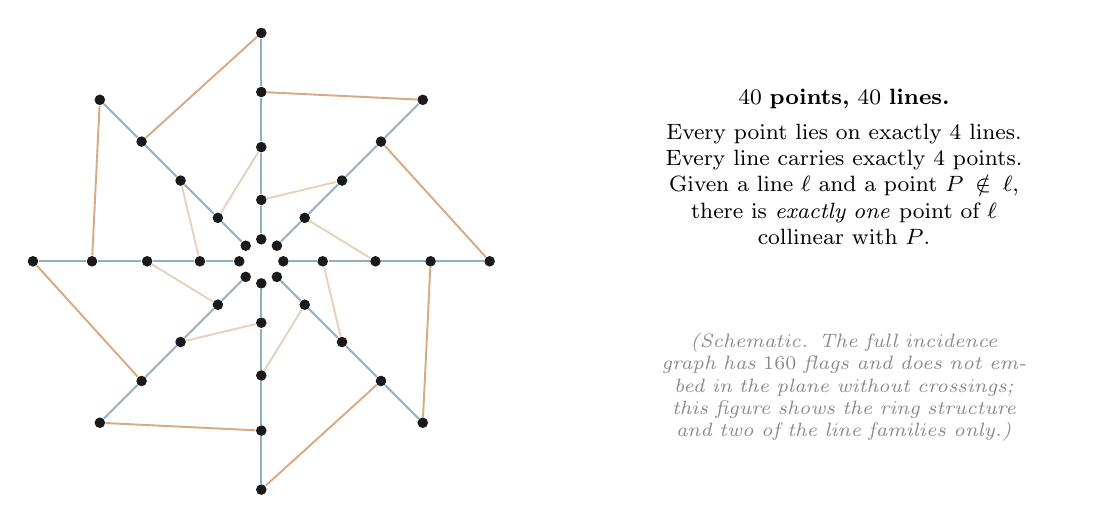
\begin{tikzpicture}[font=\footnotesize,
  pt/.style={circle,fill=ink,inner sep=1.35pt},
  ln/.style={draw=past,line width=0.7pt,opacity=0.55}]

  % a schematic of the GQ(3,3) incidence: 5 "spread" groups of 8 points on a ring
  \foreach \k in {0,...,7}{
    \pgfmathsetmacro\ang{\k*45}
    \foreach \r/\lab in {2.9/a, 2.15/b, 1.45/c, 0.78/d, 0.28/e}{
      \node[pt] (P\k\lab) at (\ang:\r) {};
    }
  }
  \foreach \k in {0,...,7}{
    \draw[ln] (P\k a) -- (P\k b) -- (P\k c) -- (P\k d) -- (P\k e);
  }
  \foreach \k [evaluate=\k as \j using {int(mod(\k+1,8))}] in {0,...,7}{
    \draw[ln,draw=future] (P\k a) -- (P\j b);
    \draw[ln,draw=future,opacity=0.3] (P\k c) -- (P\j d);
  }
  \node[align=center,text width=5.4cm] at (7.4,1.2)
   {\textbf{$40$ points, $40$ lines.}\\[3pt]
    Every point lies on exactly $4$ lines.\\
    Every line carries exactly $4$ points.\\
    Given a line $\ell$ and a point $P\notin\ell$,\\
    there is \emph{exactly one} point of $\ell$\\
    collinear with $P$.};
  \node[align=center,text width=5.4cm,font=\scriptsize,text=rule] at (7.4,-1.6)
   {\textit{(Schematic. The full incidence graph has $160$ flags and does not embed in
    the plane without crossings; this figure shows the ring structure and two of the
    line families only.)}};
\end{tikzpicture}
\end{center}

\begin{plain}
The ``exactly one'' statement is an incidence projection rule: for a point outside a
line there is one point on that line collinear with it.  It does not imply unique
shortest paths in the collinearity graph.  Each four-point line is a $K_4$, so that
graph contains triangles; the triangle-free object is the bipartite point--line
incidence graph, whose generalized-quadrangle girth is eight.  Routing claims must
therefore be proved by the routing code, not inferred from the word quadrangle.
\end{plain}

\subsection{The wiring as a budget}

\begin{plain}
One more fact about the shape, and it is the kind that makes a reader sit up --- so it
comes with an unusually careful statement of what it does \emph{not} mean.

Treat the $240$ connections as a physical system and ask how they vibrate. The answer
splits them into four groups.
\end{plain}

\begin{spec}[Hodge Laplacian on $1$-chains, recomputed independently, Pass 2884]
\[
  240 \;=\; \underbrace{81}_{\text{harmonic}} \;+\; \underbrace{120}_{\lambda=4}
       \;+\; \underbrace{24}_{\lambda=10} \;+\; \underbrace{15}_{\lambda=16}
\]
The harmonic sector has dimension $81$ --- the frame register file, and the logical
dimension of the substrate's own qutrit code $[240,81,d_Z{=}4]$.
\end{spec}

\begin{gotwrong}[What is tempting here, and why it is not claimed]
Two of the other three numbers are already architectural quantities in this document:
$15$ is the dimension of the support shell, and $24$ is the order of the single-qutrit
Clifford group modulo phase. It is very tempting to read the line above as ``the machine's
wiring decomposes into its own subsystems.''

\medskip\noindent
\textbf{No map is exhibited in either case.} These are equal integers. This project's
second most expensive failure mode is precisely an over-read of a count match --- and
\S\ref{sec:isa} contains a worked example where exactly this kind of coincidence, tested,
turned out to be nothing. The decomposition is recorded as an open question: is either
coincidence carried by a natural map? Until someone answers that, it is arithmetic.
\end{gotwrong}

\subsection{Why three?}

\begin{plain}
A fair question, and the one a sceptical reader should ask: the machine uses three-way
switches rather than two-way ones, and three-way switches are unusual. Was three chosen
because it works, or does something choose it?

The honest answer is that this project found five independent conditions that each single
out three, none of them adjustable. Here are two anyone can check by hand.
\end{plain}

\begin{spec}[Two of the five selection conditions]
\textbf{Counting.} A geometry of this type with $q$-way switches has
$q(q+1)^2(q^2+1)/2$ edges. The number of elements you gain by extending the arithmetic
five steps is $q^5-q$. Demanding these agree:
\[
  q^5-q=\frac{q(q+1)^2(q^2+1)}{2}\;\Longrightarrow\;2(q-1)=q+1\;\Longrightarrow\;
  \boxed{q=3}\ \text{uniquely}.
\]
Checked directly: $q^5-q$ for $q=2,3,4,5,7,11$ gives
$30,\,\mathbf{240},\,1020,\,3120,\,16800,\,161040$, while the edge counts are
$45,\,\mathbf{240},\,850,\,2340,\,11200,\,96624$. They meet only at three.

\smallskip\noindent
\textbf{Symmetry.} The symmetry group of the geometry and the symmetry group of the
exceptional structure $E_6$ have the same order --- $51{,}840$ --- only at $q=3$.
\end{spec}

\headline{$240 = 3^5-3$. The same $240$ is the edge count of the geometry, the number of
roots of $E_8$, and the count of non-base elements in the degree-five extension of the
three-element field. Three conditions, one number, no free parameters.}

\begin{spec}[All five, for completeness]
\begin{center}\small
\begin{tabular}{@{}rp{8.4cm}l@{}}
\toprule
\# & condition & forces\\
\midrule
1 & $q^5-q$ equals the $GQ(q,q)$ edge count & $q=3$ uniquely\\
2 & $\sin^2\theta_W = 3/8$ at unification & $3q^2-10q+3=0\Rightarrow q=3$\\
3 & $K_{q+1}$ has exactly $q$ perfect matchings & only $q=3$: $K_4$ has $3$\\
4 & non-neighbours $=\dim(E_6$ fundamental$)$ & $v-k-1=q^3=27\Rightarrow q=3$\\
5 & $|\mathrm{PGSp}(4,q)| = |W(E_6)|$ & the order equality selects $q=3$\\
\bottomrule
\end{tabular}
\end{center}
Every one has $q$ as an integer unknown and exactly one positive solution. Prior art:
\cmd{docs/index.html} owns all five.
\end{spec}

\begin{plain}
Three more conditions in the same family --- involving the electroweak mixing angle at
unification, the number of perfect matchings of a small complete graph, and the dimension
of the fundamental representation of $E_6$ --- also give three and only three. None of
them was fitted; $q$ appears in each as an integer to be solved for, and each equation has
exactly one positive integer solution.

That does not make three \emph{necessary} in any deep sense we can prove. It does mean the
machine's most unusual design choice is not a preference.
\end{plain}

\subsection{The two groups of order $51{,}840$, which are not the same group}

\begin{spec}
Two distinct groups of order $51{,}840$ appear in this project, and confusing them is the
most common error in this area:
\[
  \mathrm{Sp}(4,3)=2.U_4(2)\quad(\text{centre of order }2),\qquad
  \mathrm{PGSp}(4,3)=U_4(2){:}2=W(E_6)\quad(\text{trivial centre}).
\]
They are \emph{not} isomorphic. The first is the group acting on Pauli frames --- the one
the hardware implements. The second is the automorphism group of the geometry --- the one
the drawing has. One is a central double cover; the other is an outer extension.
\end{spec}

\begin{plain}
This distinction is not pedantry, and it has physical content. The extra element in the
first group acts as a sign, $z\mapsto -1$. Whether that sign is ``spent'' or ``free''
decides whether the resulting structure has a handedness --- whether it distinguishes
left from right. This is why the machine can \emph{host} a chirality, though as we
established in earlier work it cannot \emph{explain} one from the inside.
\end{plain}

% =====================================================================================

% =====================================================================================
\section{Four representations, four jobs}\label{sec:representations}
% =====================================================================================

\begin{plain}
The machine now has four compact descriptions of the same underlying frame, and they must
not be confused.  The seven-bit code is the execution state.  The four-bit support mask is
cheap one-way telemetry.  The protected observer words trade more wires and time for error
correction.  The ninety-six-state selector--tomotope token is a control word, not stored
quantum data.  Earlier drafts occasionally used the word ``state'' for all four; this
section removes that ambiguity from the architecture.
\end{plain}

\begin{spec}[Representation contract]
\begin{description}[leftmargin=2.4cm,style=nextline,font=\normalfont\bfseries]
\item[Affine frame]
  $7$ bits. Lossless for all $81$ Pauli frames; execution may read and write it.
\item[Support telemetry]
  $4$ bits. Zero/nonzero mask only, and frame $\to$ support is one-way
  in the netlist --- proved at the gate level, not asserted.
\item[Protected observer]
  $24$--$28$ taps. Diagnostic word for identification and correction; never
  the live datapath.
\item[Control token]
  $7$ raw bits, $96$ valid. Selects face, matching channel and phase cell.
\end{description}
\end{spec}

\begin{gotwrong}[Support is observable, not executable]
The refinement count $16\to40\to78\to81$ was once easy to read as four increasingly
accurate compressed machine states.  It is not.  Exhausting every nonempty subset of the
four-operation micro-ISA proves that the coarsest exact support-refining execution
quotient for the full ISA has all $81$ singleton classes.  The intermediate partitions
are observer states only.  In fact $F_p$, $Z_p$, and either controlled-add direction
already force the full frame.
\end{gotwrong}

\begin{spec}[Intrinsic selector channel]
For a noncollinear pair $x,y$ and a distinguished common neighbour $c$, the three residual
selector channels form the affine line $C(x,y)\setminus\{c\}$.  The multiplier-one
stabilizer induces its translation group $C_3$; the full projective similitude stabilizer
induces $\operatorname{AGL}(1,3)\cong S_3$.  There is therefore no globally equivariant
numbering $0,1,2$.  Hardware may choose a local encoding, but interfaces transport it as
an affine-line torsor rather than pretending the labels are geometric invariants.
\end{spec}

\clearpage
\begin{center}
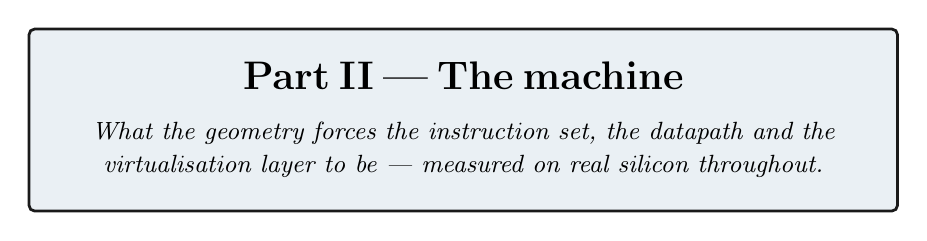
\begin{tikzpicture}
  \node[draw=ink,line width=1pt,rounded corners=2pt,inner sep=12pt,
        text width=0.84\linewidth,align=center,fill=specbg]
  {\Large\bfseries Part II  --- The machine\\[6pt]
   \normalfont\small\itshape What the geometry forces the instruction set, the datapath and the virtualisation layer to be --- measured on real silicon throughout.};
\end{tikzpicture}
\end{center}
\vspace{4mm}


% ======================================================================
\part{The Machine}

\begin{plain}[What this part is]
The computer proper --- its instructions, its register, its gate count, and the
physical layer that would run it. Everything here is either measured from a synthesised
netlist or derived exactly from the geometry of Part II, and each claim says which.
\end{plain}

\section{The instruction set}\label{sec:isa}
% =====================================================================================

\subsection{The idea of a Pauli frame}

\begin{plain}
Here is the trick that makes the machine cheap.

A quantum state is expensive to write down: for two qutrits you need nine complex
numbers, and keeping them accurate is most of what makes quantum computing hard. But for
a large and useful family of operations --- the \emph{Clifford} operations --- you never
need the state at all. You only need a \emph{label} saying how the state has been shifted
relative to where it started.

That label is four trits. Four trits is eight bits. The machine's entire ``register
file'' for tracking Clifford operations is one byte.
\end{plain}

\headline{The frame unit tracks a label, not a state. Four trits, $81$ possible values,
eight bits of memory --- and it correctly accounts for a group of $4{,}199{,}040$
distinct operations.}

\begin{plain}
That $81$ is worth pausing on, because it turns up somewhere it has no obvious business
being.

Treat the geometry as a shape and ask a purely topological question --- how many
independent loops does it have? The answer is that its first homology group is exactly
$\mathbb{Z}^{81}$: eighty-one independent cycles. Nothing about that computation mentions
registers, instructions, or qutrits. It is the same number as the size of the machine's
register file.
\end{plain}

\begin{spec}[The coincidence, and the answer]
\[
  H_1\bigl(W(3,3);\mathbb{Z}\bigr)=\mathbb{Z}^{81},
  \qquad
  |\mathbb{F}_3^4| = 81 .
\]
Both are $3^4$, and the shared exponent is not an accident: the geometry lives in a
four-dimensional space over a three-element field, and both counts are governed by that.
The clique complex over $\mathbb{F}_3$ is moreover an exact qutrit error-correcting code
with parameters $[240,81,d_Z{=}4]$ --- so the same $81$ is also the number of
\emph{protected} logical values the substrate carries.

\smallskip\noindent
\textbf{But the two spaces are not the same object} (Pass 2883). Ask whether the symmetry
group sees them alike: an order-three linear opcode fixes exactly $27$ of the $81$ frames,
while the homology character on every order-three class is $0$. The characters disagree,
so there is \emph{no} equivariant isomorphism. The counts match for a real reason and the
spaces still differ --- which is the most common shape a numerical coincidence takes in
this project, and the reason every one of them gets this test.
\end{spec}

\begin{plain}
It would have been more satisfying if the answer were yes. Writing down the negative
result is the point of having the test at all: an earlier draft of this page left the
question open, which reads as promising, and open questions that stay open too long start
to be cited as though they were answered.
\end{plain}

\begin{spec}
The Pauli frame is $(x_p,z_p,x_f,z_f)\in\mathbb{F}_3^4$, denoting the operator
$X^{x_p}Z^{z_p}\otimes X^{x_f}Z^{z_f}$. A Clifford unitary $U$ acts on frames by
conjugation, $U(X^aZ^b)U^\dagger = X^{a'}Z^{b'}$ up to phase, and the induced map on
$\mathbb{F}_3^4$ is \emph{linear and symplectic}: it preserves
\[
  \langle u,v\rangle \;=\; (x_p z_p' - z_p x_p') + (x_f z_f' - z_f x_f') \bmod 3 .
\]
\end{spec}

\subsection{The eight opcodes}

\begin{spec}[$\mathcal{I}_{\mathrm{holo}}$, complete semantics]
\begin{center}\small
\begin{tabular}{@{}llll@{}}
\toprule
\textbf{Op} & \textbf{Name} & \textbf{Action on $(x_p,z_p,x_f,z_f)$} & \textbf{Kind}\\
\midrule
\texttt{000} & $F_p$ & $(x_p,z_p)\mapsto(-z_p,\;x_p)$              & linear \\
\texttt{001} & $F_f$ & $(x_f,z_f)\mapsto(-z_f,\;x_f)$              & linear \\
\texttt{010} & $S_p$ & $z_p\mapsto z_p+x_p$                        & linear \\
\texttt{011} & $S_f$ & $z_f\mapsto z_f+x_f$                        & linear \\
\texttt{100} & $\mathrm{CX}$ & $d{=}0$: $z_p\mapsto z_p-z_f$, $x_f\mapsto x_f+x_p$
                              & linear \\
             &               & $d{=}1$: $x_p\mapsto x_p+x_f$, $z_f\mapsto z_f-z_p$
                              & linear \\
\texttt{101} & $\sigma^5{=}Z$ & $z_p\mapsto z_p+1$ \ or\  $z_f\mapsto z_f+1$
                              & \textbf{affine} \\
\texttt{110} & $D_{12}$-mirror & transport in the dihedral group $D_{12}$ & (not a frame op)\\
\texttt{111} & $M_{36}$-magic & typed request for one of $36$ Witting rays & (handshake)\\
\bottomrule
\end{tabular}
\end{center}
\end{spec}

\subsection{The reachability theorem, and why it matters}

\begin{plain}
Now a question that sounds trivial and is not: \emph{starting from a blank machine, which
states can these instructions actually reach?}

The answer is startling. All six of the Clifford instructions, applied in any order, any
number of times, reach exactly \emph{one} state --- the blank one. They cannot move the
machine at all.

The reason is simple once you see it. Those six instructions are all \emph{linear}, and a
linear map always leaves the origin where it is. Multiplying zero by anything gives zero.
So a machine built from only those six instructions is, quite literally, a machine that
does nothing, no matter how sophisticated its circuitry looks.

The seventh instruction, $\sigma^5=Z$, is different: it \emph{adds one}. Addition moves
the origin. That single instruction is what makes all $81$ states reachable --- and hence
what makes the machine a computer instead of an ornament.
\end{plain}

\begin{center}
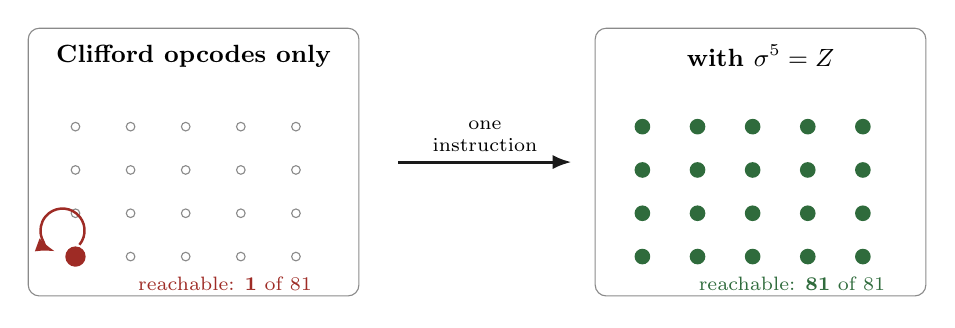
\begin{tikzpicture}[font=\small,>={Latex[length=2.4mm]}]
  % left: clifford only
  \begin{scope}
    \draw[draw=rule,rounded corners] (-0.6,-1.5) rectangle (3.6,1.9);
    \node[font=\bfseries\small] at (1.5,1.55) {Clifford opcodes only};
    \foreach \x in {0,...,4}\foreach \y in {0,...,3}{
      \node[circle,draw=rule,inner sep=1.1pt,fill=white] at (0.7*\x,0.55*\y-1.0) {};}
    \node[circle,fill=bad,inner sep=2.6pt] at (0,-1.0) {};
    \draw[->,line width=0.9pt,draw=bad] (0.05,-0.85) arc (-40:250:0.28);
    \node[font=\scriptsize,text=bad,align=center] at (1.9,-1.35)
      {reachable: \textbf{1} of $81$};
  \end{scope}
  % right: with Z
  \begin{scope}[xshift=7.2cm]
    \draw[draw=rule,rounded corners] (-0.6,-1.5) rectangle (3.6,1.9);
    \node[font=\bfseries\small] at (1.5,1.55) {with $\sigma^5=Z$};
    \foreach \x in {0,...,4}\foreach \y in {0,...,3}{
      \node[circle,fill=good,inner sep=2.0pt] at (0.7*\x,0.55*\y-1.0) {};}
    \node[font=\scriptsize,text=good,align=center] at (1.9,-1.35)
      {reachable: \textbf{81} of $81$};
  \end{scope}
  \draw[->,line width=1.1pt,draw=ink] (4.1,0.2) -- (6.3,0.2)
    node[midway,above,font=\scriptsize,align=center] {one\\instruction};
\end{tikzpicture}
\end{center}

\begin{spec}[Proved by exhaustive search, Pass 2774]
Breadth-first search over all $3^4=81$ frames from $(0,0,0,0)$:
\[
\begin{array}{lr}
\textrm{$\mathrm{CX}$ alone} & 1 \\
\textrm{all six symplectic opcodes} & 1 \\
\textrm{full ISA (adding $\sigma^5{=}Z$)} & 81 \\
\end{array}
\]
Reproduce: \cmd{py -3 analysis/w33\_pass2774\_isa\_frame\_reachability.py}\\
Certificate: \cmd{data/PART\_W33\_PASS2774\_ISA\_FRAME\_REACHABILITY.json}
\end{spec}

\subsection{How much computation the eight opcodes actually buy}

\begin{plain}
``All $81$ states are reachable'' is weaker than it sounds --- it says you can get
anywhere, not that you can perform every operation. The stronger question is: what is the
complete list of things this instruction set can do?
\end{plain}

\begin{spec}[Proved, Pass 2778]
The six Clifford opcodes generate a group of order exactly $51{,}840$ --- that is, the
whole of $\mathrm{Sp}(4,3)$, nothing missing. Adjoining the translation gives
\[
  \langle \mathcal{I}_{\mathrm{holo}}\rangle
   \;=\; \mathrm{ASp}(4,3)\;=\;\mathbb{F}_3^4\rtimes\mathrm{Sp}(4,3),
  \qquad |\cdot| = 81\times 51840 = 4{,}199{,}040 .
\]
\textbf{One translation generator suffices.} Enabling only $Z$ on the past register gives
the same group as enabling both, because $\mathrm{Sp}(4,3)$ is transitive on the $80$
nonzero frame vectors: the orbit of a single translation already spans $\mathbb{F}_3^4$.
Measured orbit size: $80$. A second translation instruction adds nothing and can be
removed from the ISA.
\end{spec}

\headline{Eight opcodes. Three bits. $4{,}199{,}040$ distinct operations, exactly ---
and the eighth opcode is provably redundant.}

\subsection{How small can the instruction set be?}

\begin{plain}
If one opcode is redundant, how many are? This is not idle: every instruction removed is
decoder logic removed, and if enough go, the opcode field itself gets shorter --- which
shortens every instruction word in the machine.

The answer is that you can throw away half of them.
\end{plain}

\begin{spec}[Exhaustive over all subsets, Pass 2789]
Because $\mathbb{F}_3^4\rtimes H=\mathrm{ASp}(4,3)$ iff $H=\mathrm{Sp}(4,3)$ and at least
one translation is present, the search reduces to the six linear opcodes:
\[
\begin{array}{ll}
\text{subsets of size }1\text{ generating }\mathrm{Sp}(4,3): & 0\\
\text{subsets of size }2: & 0\\
\text{subsets of size }3: & \mathbf{6}
\end{array}
\]
The six minimal triples are
$\{F_p,F_f,\mathrm{CX}_{p\to f}\}$, $\{F_p,F_f,\mathrm{CX}_{f\to p}\}$,
$\{F_p,S_f,\mathrm{CX}_{p\to f}\}$, $\{F_p,\mathrm{CX}_{p\to f},\mathrm{CX}_{f\to p}\}$,
$\{F_f,S_p,\mathrm{CX}_{f\to p}\}$, $\{F_f,\mathrm{CX}_{p\to f},\mathrm{CX}_{f\to p}\}$.
\end{spec}

\headline{Three Clifford opcodes plus one translation generate everything.
Four frame instructions --- a \textbf{two-bit} opcode field, not three.}

\begin{plain}
Six choices, all valid --- so pick whichever is cheapest to build, and the decision costs
nothing. That was the obvious inference, and it is wrong.
\end{plain}

\begin{spec}[The six triples do \emph{not} cost the same, Pass 2882]
Exhaustive breadth-first search over the full group, once per triple:
\begin{center}\small
\begin{tabular}{@{}lrr@{}}
\toprule
triple & diameter & mean\\
\midrule
$F_p + \mathrm{CX}_{p\to f} + \mathrm{CX}_{f\to p}$ & \textbf{19} & \textbf{14.18}\\
$F_f + \mathrm{CX}_{p\to f} + \mathrm{CX}_{f\to p}$ & 20 & 15.22\\
$F_p + F_f + \mathrm{CX}_{f\to p}$ & 22 & 16.08\\
$F_p + S_f + \mathrm{CX}_{p\to f}$ & 22 & 16.12\\
$F_f + S_p + \mathrm{CX}_{f\to p}$ & 22 & 15.90\\
$F_p + F_f + \mathrm{CX}_{p\to f}$ & 23 & 17.08\\
\bottomrule
\end{tabular}
\end{center}
\end{spec}

\headline{Worst-case program length varies from \textbf{19 to 23} across the six ---
a $21\%$ spread for a choice that looks free. Build the one with two entanglers.}

\begin{plain}
The pattern is legible once seen: the best triple is the one containing \emph{both}
directions of the coupling instruction, and the worst is the one containing neither. What
shortens programs is the ability to move information both ways between past and future,
which is a satisfying thing for the machine's own central metaphor to be rewarded by its
compiler.
\end{plain}

\subsection{How long is the longest program?}

\begin{plain}
``These four operations can do everything'' is a statement about what is \emph{possible}.
The question a compiler actually asks is what it \emph{costs}: if I hand you an arbitrary
frame transformation, how many instructions do you need in the worst case?

That number is the machine's \emph{diameter}, and it can be computed exactly, because the
group is only four million elements and a computer can visit all of them.
\end{plain}

\begin{spec}[Exhaustive breadth-first search over $\mathrm{ASp}(4,3)$, Pass 2866]
Forward generators only --- a processor cannot run an instruction backwards, so the
\emph{directed} diameter is the honest number.
\[
  \boxed{\text{diameter}=19},\qquad
  \text{mean program length}=14.176,\qquad
  \text{counting floor }\lceil\log_4 4199040\rceil=12 .
\]
The last shell is tiny: only $188$ of $4{,}199{,}040$ elements are at distance exactly
$19$. Ball sizes reach $93.3\%$ at depth $16$ and $99.996\%$ at depth $18$.
\end{spec}

\headline{Every frame transformation is at most \textbf{19} instructions away, and the
average is \textbf{14.2}. No four-operation instruction set can beat $12$, so this one is
worst-case optimal to within a factor of $1.73$.}

\begin{plain}
The method is worth a sentence because it is what makes the computation possible at all. A
group element is a matrix together with a shift. Each instruction acts on the matrix part
as a fixed \emph{shuffle} of $51{,}840$ labels and on the shift part as a fixed map of $81$
labels. Build those two lookup tables once, and searching four million elements is just
table lookups --- seconds, not days.
\end{plain}

\subsection{And how long until the machine forgets?}

\begin{plain}
The opposite question. Feed the machine random instructions: how many before its state
tells you nothing about where it started?
\end{plain}

\begin{spec}[Exact, Pass 2867]
Every opcode is a bijection on the $81$ frames, so the walk is doubly stochastic and the
stationary distribution is exactly uniform --- \emph{no frame is preferred}.
\[
  |\lambda_2| = 0.893992,\qquad
  \text{gap}=0.106008,\qquad
  \frac{1}{\text{gap}}=9.43,\qquad
  t_{\mathrm{mix}}(\tfrac14)=15,\qquad
  K=113.38 .
\]
\end{spec}

\headline{A frame forgets its origin by $1/e$ in $9.4$ instructions and is statistically
gone after $15$ --- \textbf{$71.8$\,ns} at the measured $208.86$\,MHz.}

\begin{spec}[And what the worst case actually looks like, Pass 2885]
Only $188$ of $4{,}199{,}040$ elements sit at distance exactly $19$ --- $0.0045\%$. The
natural guess is that so rare a set is one orbit, one coset, something nameable.

\smallskip\noindent
\textbf{It is not.} Those $188$ spread over $54$ distinct linear parts, element orders $4$
through $18$, and all three trace classes. There is no single ``hardest instruction'' to
name, and the structural hypothesis is refuted.

\smallskip\noindent
What survives is the useful half: \textbf{$188$ is small enough to enumerate exactly}, so
a compiler regression suite can contain \emph{every} worst-case input rather than sampling
for them. A negative structural result and a positive engineering one out of the same run.
\end{spec}

\begin{plain}
Put that beside the readout cost of \S\ref{sec:support} and you get an observation
cadence, which is a real design parameter: reading more often than every fifteen
instructions pays the thermodynamic price repeatedly for information the machine has not
yet regenerated.

Notice also how close $15$ and $19$ are. The machine scrambles almost exactly as fast as
it can reach --- there is no regime in which it is still reachable but already random,
which is a comfortable property for a scheduler to have.
\end{plain}

\begin{gotwrong}[A trap avoided, and worth naming]
A minimality \emph{proof} says nothing about \emph{area}. It is tempting to quote the
$72$-cell figure for the four-operation engine on the grounds that it does strictly less
work --- and that would be wrong twice over: the number was measured on a different
design, and removing decode cases can \emph{cost} cells when what was removed was being
shared with what remains. The minimal engine was therefore synthesised and placed
separately (\S\ref{sec:budget}), and only then quoted. It came out at $43$ cells; had it
come out at $80$, that is the number this document would print.
\end{gotwrong}

\begin{plain}
Two details are worth noticing. First, there are \emph{six} different minimal choices, so
a chip designer has real freedom to pick whichever three are cheapest in silicon rather
than being handed one answer.

Second, every single one of the six contains at least one Fourier gate \emph{and} at
least one controlled-add. No collection of phase gates and one Fourier gate will do. The
entangler is not optional --- which is the formal version of the intuition that a machine
that never couples past to future is not really using the self-entanglement at all.
\end{plain}

% =====================================================================================
\section{The hardware}\label{sec:hardware}
% =====================================================================================

\subsection{The frame unit datapath}
\begin{plain}
This is the circuit diagram of the register itself --- the part of the machine that actually
holds a number. Four small boxes across the top store the four coordinates; the shapes below
them are the arithmetic that adds and multiplies modulo three; the funnel symbols are
switches choosing which instruction is being carried out this cycle. The single box on the
right marked \emph{load port} is the only way a value ever enters from outside, and
\S\ref{sec:pbias} is about the consequences of it being there.
\end{plain}


\begin{center}
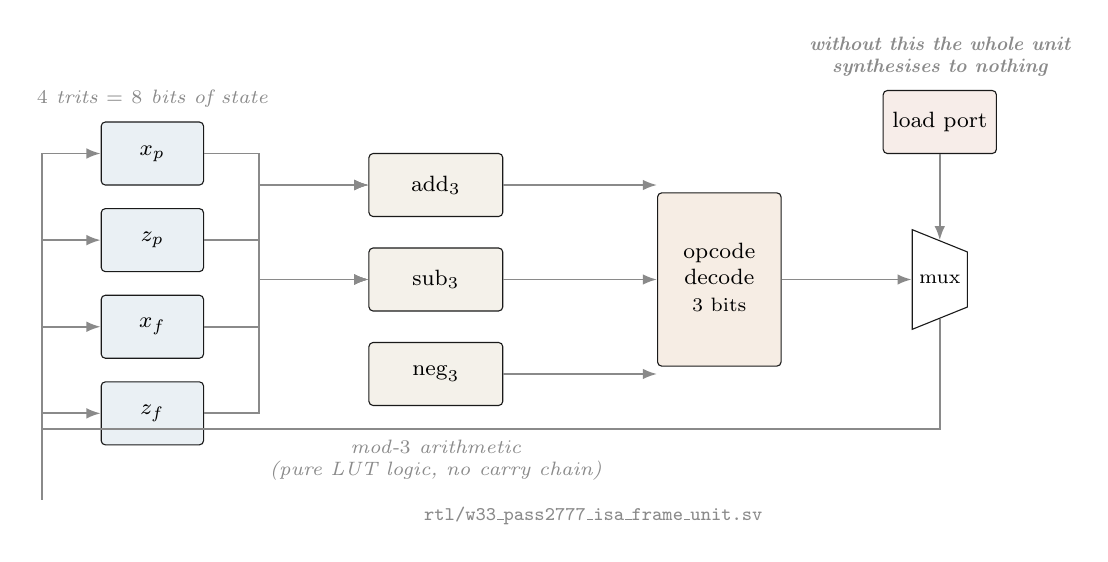
\begin{tikzpicture}[font=\footnotesize,>={Latex[length=2.2mm]},
  reg/.style={draw=ink,fill=specbg,minimum width=13mm,minimum height=8mm,rounded corners=1.5pt},
  alu/.style={draw=ink,fill=plainbg,minimum width=17mm,minimum height=8mm,rounded corners=1.5pt},
  mux/.style={draw=ink,fill=white,trapezium,trapezium angle=68,minimum width=9mm,
              minimum height=7mm,shape border rotate=270,inner sep=1pt},
  w/.style={-{Latex[length=1.8mm]},draw=rule,line width=0.7pt}]

  % registers
  \node[reg] (xp) at (0,3.0)  {$x_p$};
  \node[reg] (zp) at (0,1.9)  {$z_p$};
  \node[reg] (xf) at (0,0.8)  {$x_f$};
  \node[reg] (zf) at (0,-0.3) {$z_f$};
  \node[font=\scriptsize\itshape,text=rule,above=0.5mm of xp] {$4$ trits $=$ $8$ bits of state};

  % f3 units
  \node[alu] (a1) at (3.6,2.6) {$\mathrm{add}_3$};
  \node[alu] (a2) at (3.6,1.4) {$\mathrm{sub}_3$};
  \node[alu] (a3) at (3.6,0.2) {$\mathrm{neg}_3$};
  \node[font=\scriptsize\itshape,text=rule,align=center] at (3.6,-0.9)
    {mod-$3$ arithmetic\\(pure LUT logic, no carry chain)};

  % opcode decode
  \node[alu,minimum height=22mm,minimum width=15mm,fill=future!12] (dec) at (7.2,1.4)
    {\begin{tabular}{c}opcode\\decode\\\scriptsize $3$ bits\end{tabular}};

  % next-state mux
  \node[mux] (m) at (10.0,1.4) {};
  \node[font=\scriptsize] at (10.0,1.4) {mux};

  \node[reg,fill=warnbg] (ld) at (10.0,3.4) {load port};
  \node[font=\scriptsize\itshape,text=rule,align=center,above=0.5mm of ld]
    {\textbf{without this the whole unit}\\\textbf{synthesises to nothing}};

  \foreach \r in {xp,zp,xf,zf}{
    \draw[w] (\r.east) -- ++(0.7,0) |- (a1.west);
    \draw[w] (\r.east) -- ++(0.7,0) |- (a2.west);
  }
  \draw[w] (a1.east) -- (dec.west|-a1);
  \draw[w] (a2.east) -- (dec.west|-a2);
  \draw[w] (a3.east) -- (dec.west|-a3);
  \draw[w] (dec.east) -- (m.west);
  \draw[w] (ld.south) -- (m.north);
  \draw[w] (m.south) |- ++(0,-1.4) -| (-1.4,-1.4) |- (xp.west);
  \draw[w] (-1.4,-1.4) |- (zp.west);
  \draw[w] (-1.4,-1.4) |- (xf.west);
  \draw[w] (-1.4,-1.4) |- (zf.west);

  \node[font=\scriptsize,text=rule] at (5.6,-1.6)
    {\cmd{rtl/w33\_pass2777\_isa\_frame\_unit.sv}};
\end{tikzpicture}
\end{center}

\subsection{The measured cell budget}\label{sec:budget}

\begin{plain}
Below is what the machine actually costs, measured by running the industry-standard
open-source tools --- Yosys to translate the design into logic gates, nextpnr to place
those gates on a real chip --- targeting a Lattice iCE40 UP5K, a chip you can buy on a
breakout board for about \$25.

The entire arithmetic core of this computer is \emph{seventy-two} logic cells, out of
$5{,}280$ available. It uses $1.4\%$ of a \$25 chip.
\end{plain}

\begin{spec}[The three designs, on two parts, in one harness]
\begin{center}\small
\begin{tabular}{@{}lrrrrl@{}}
\toprule
 & \multicolumn{2}{c}{\textbf{HX8K CT256}} & \multicolumn{2}{c}{\textbf{UP5K SG48}} & \\
\cmidrule(lr){2-3}\cmidrule(lr){4-5}
\textbf{Design} & \textbf{LC} & \textbf{$F_{\max}$} & \textbf{LC} & \textbf{$F_{\max}$}
                & \textbf{Opcode}\\
\midrule
Minimal engine, $4$ operations & \textbf{43} & \textbf{208.86} & 43 & 72.40 & 2 bits\\
Public unit, $6$ frame opcodes & 72 & 175.72 & 72 & 60.80 & 3 bits\\
Engine $+$ support readout     & 48 & 207.64 & 48 & 72.05 & 2 bits\\
\bottomrule
\end{tabular}\\[3pt]
\itshape\footnotesize frequencies in MHz
\end{center}
Same cells on both parts --- synthesis does not know the package --- but the HX8K is
$2.9\times$ faster. \textbf{Every UP5K figure elsewhere in this document therefore
understates speed by about a factor of three}, and is kept because it is the part the
$\$25$ board carries.
\end{spec}

\begin{spec}[Measured on UP5K SG48; the per-instruction breakdown]
\begin{center}\small
\begin{tabular}{@{}lrrrl@{}}
\toprule
\textbf{Design} & \textbf{Cells} & \textbf{Pins} & \textbf{$F_{\max}$} & \textbf{Opcode}\\
\midrule
Minimal engine, $4$ operations & \textbf{43} & 22 & \textbf{72.40}\,MHz & 2 bits \\
Public unit, $6$ frame opcodes & 72 & 26 & 60.80\,MHz & 3 bits \\
\bottomrule
\end{tabular}
\end{center}
\textbf{$40\%$ fewer cells and $19\%$ faster.} The minimality theorem cashes out in
silicon. Also verified on the minimal engine, because both checks are cheap and both have
caught real defects here: the linear part is symplectic on frame \emph{differences}
(SAT, $4100$ variables / $11278$ clauses --- a translation cancels in a difference, so one
assertion covers all four opcodes at once), and no output folds to a constant.
\end{spec}

\begin{spec}[Measured; iCE40 UP5K SG48, Yosys 0.67 $+$ nextpnr]
\begin{center}\small
\begin{tabular}{@{}lrrl@{}}
\toprule
\textbf{Build} & \textbf{Logic cells} & \textbf{$F_{\max}$ (MHz)} & \textbf{Contains}\\
\midrule
$F$ only                 & 16 & 230.84 & one Fourier gate \\
$F_p + F_f$              & 19 & 230.84 & both Fourier gates \\
$F$ and $S$ (4 opcodes)  & 40 &  86.60 & the single-qutrit Cliffords \\
$\mathrm{CX}$ only       & 33 &  72.40 & the entangler, both directions \\
$\sigma^5{=}Z$ only      & 20 & 144.07 & the translation \\
all Clifford, no $Z$     & 65 &  60.80 & \textcolor{bad}{cannot leave the origin} \\
\textbf{full frame unit} & \textbf{72} & \textbf{60.80} & \textcolor{good}{the machine} \\
\midrule
\multicolumn{4}{@{}l}{\itshape For comparison, elsewhere in the design:}\\
$\mathrm{CX}$, bare loadable        &  23 & 72.40 & \cmd{w33\_pass2752\_cx\_loadable\_frame.sv}\\
$36$-lane mixer, serial            & 4048 & 19.65 & \cmd{w33\_pass2612\_serial\_mixer.sv}\\
$36$-lane mixer, parallel          & \multicolumn{2}{l}{13{,}965 LUT4 $+$ 799 carry} &
    \textcolor{bad}{does not fit any iCE40}\\
\bottomrule
\end{tabular}
\end{center}
\end{spec}

\begin{plain}
The last two rows are worth a moment. The ``mixer'' is the part that combines $36$
signals at once. Built the obvious way --- all $36$ lanes in parallel --- it needs
about $14{,}000$ logic cells, nearly twice what the largest chip in this family has. Built
serially, one lane at a time, it needs $4{,}048$: about a third of the area, at
$1/36$ of the speed. That is the kind of trade a blueprint exists to make explicit.
\end{plain}

\begin{gotwrong}
\textbf{Every cell count in this project before Pass 2753 was wrong, and the reason is
instructive.} We reported $13$ cells for $F$ and $S$, $8$ for $\mathrm{CX}$, $42$ for the
ISA. Those modules had no load port. By the reachability theorem of \S\ref{sec:isa}, a
register driven only by Clifford opcodes can never leave $(0,0,0,0)$ --- so the synthesis
tool \emph{proved the state was constant and deleted six of the eight flip-flops}. We were
measuring the area of nothing.

\medskip\noindent
Two independent teams shipped this same defect within four hours of each other. Both had
\emph{exhaustive} testbenches --- one covered all $81^2$ pairs of frames --- and both
passed, because the testbenches drove the \emph{combinational} logic and never
instantiated the sequential wrapper.

\medskip\noindent
\textbf{Simulation cannot detect this class of defect at all.} A module that folds to a
constant still simulates correctly. It just does nothing. Only a synthesis frontend asks
whether the state can move.

\medskip\noindent
One figure survived unchanged: $\sigma^5=Z$ was reported at $21$ cells and re-measures at
$20$. It was always real --- because it is the one instruction that is not linear, and so
the one instruction that could always move the state. The theory predicted exactly which
number would survive.
\end{gotwrong}

% =====================================================================================
\clearpage
\begin{center}
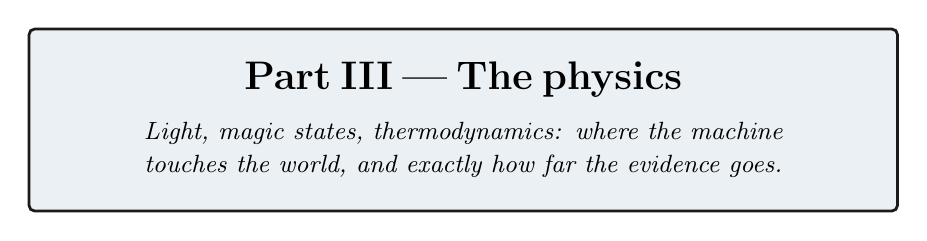
\begin{tikzpicture}
  \node[draw=ink,line width=1pt,rounded corners=2pt,inner sep=12pt,
        text width=0.84\linewidth,align=center,fill=specbg]
  {\Large\bfseries Part III  --- The physics\\[6pt]
   \normalfont\small\itshape Light, magic states, thermodynamics: where the machine touches the world, and exactly how far the evidence goes.};
\end{tikzpicture}
\end{center}
\vspace{4mm}

\section{The physical layer}
% =====================================================================================

\begin{plain}
Everything above is logic --- it would work on any hardware that can implement the eight
operations. This section is about doing it with light, which is the intended
implementation, and about what has already been demonstrated in a laboratory as opposed
to designed on paper.

A single photon carries several independent properties. Two of them are useful here:
\emph{when} it arrives (its time bin) and \emph{what colour} it is (its frequency bin).
Chop time into three slots and colour into three bands, and one photon carries two
qutrits --- the ``past'' and ``future'' registers of \S\ref{sec:physics}.
\end{plain}

\begin{center}
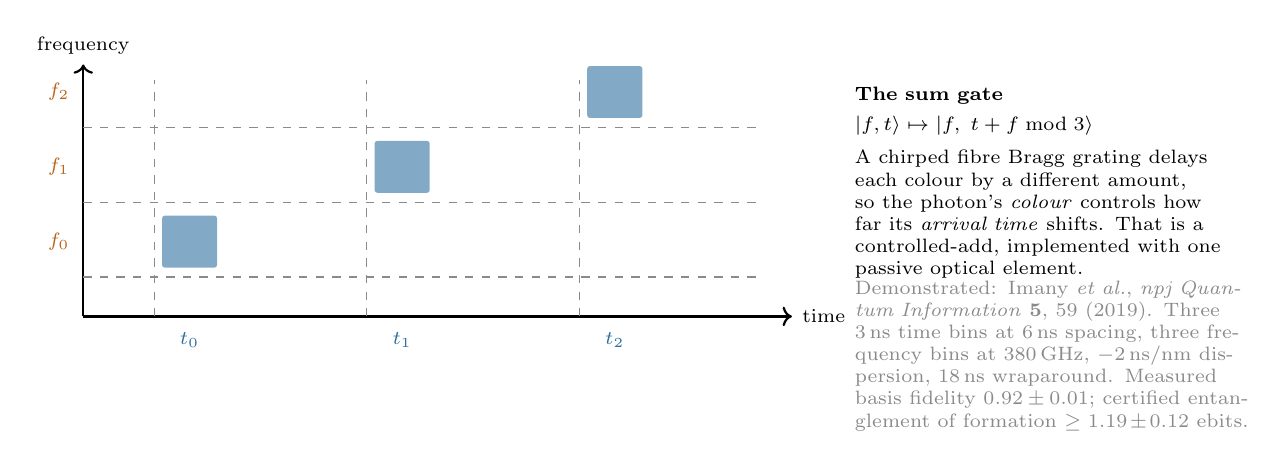
\begin{tikzpicture}[font=\footnotesize]
  \draw[->,line width=0.8pt] (0,0) -- (9.0,0) node[right,font=\scriptsize] {time};
  \draw[->,line width=0.8pt] (0,0) -- (0,3.2) node[above,font=\scriptsize] {frequency};
  \foreach \i in {0,1,2}{
    \draw[dashed,draw=rule] (0,\i*0.95+0.5) -- (8.6,\i*0.95+0.5);
    \draw[dashed,draw=rule] (\i*2.7+0.9,0) -- (\i*2.7+0.9,3.0);
  }
  \foreach \i in {0,1,2}{
    \node[font=\scriptsize,text=future,left] at (-0.05,\i*0.95+0.95) {$f_\i$};
    \node[font=\scriptsize,text=past,below] at (\i*2.7+1.35,-0.08) {$t_\i$};
  }
  \foreach \i in {0,1,2}{
    \fill[past!60,rounded corners=1pt]
      (\i*2.7+1.0,\i*0.95+0.62) rectangle (\i*2.7+1.7,\i*0.95+1.28);
  }
  \node[align=left,text width=5.0cm,font=\scriptsize] at (12.3,1.7)
   {\textbf{The \textsc{sum} gate}\\[3pt]
    $\ket{f,t}\mapsto\ket{f,\;t+f \bmod 3}$\\[4pt]
    A chirped fibre Bragg grating delays each colour by a different amount, so the
    photon's \emph{colour} controls how far its \emph{arrival time} shifts. That is a
    controlled-add, implemented with one passive optical element.};
  \node[align=left,text width=5.0cm,font=\scriptsize,text=rule] at (12.3,-0.5)
   {Demonstrated: Imany \emph{et al.}, \emph{npj Quantum Information} \textbf{5}, 59
    (2019). Three $3$\,ns time bins at $6$\,ns spacing, three frequency bins at
    $380$\,GHz, $-2$\,ns/nm dispersion, $18$\,ns wraparound. Measured basis fidelity
    $0.92\pm0.01$; certified entanglement of formation $\ge 1.19\pm0.12$ ebits.};
\end{tikzpicture}
\end{center}

\begin{spec}[Evidence boundary --- what is measured and what is not]
\textbf{Measured in a laboratory:} the deterministic single-photon qutrit \textsc{sum}
gate, at fidelity $0.92\pm0.01$, with the entangled output certified.

\smallskip\noindent
\textbf{Proved exactly:} the group theory, the geometry, the class atlas, the ISA
semantics, the reachability, the synthesis and placement figures.

\smallskip\noindent
\textbf{Neither, and stated as such:} source efficiency, insertion-loss engineering,
fault-tolerance thresholds, and the magic-state injection route. The $M_{36}$ resources
are typed \cmd{M36\_Q4\_RAW} in the controller and injection is \emph{refused} in RTL
until a proved ququart protocol supplies a validity assertion. That refusal is a design
feature: it makes the gap impossible to paper over.
\end{spec}

% =====================================================================================
\section{Why the exponent nine}
% =====================================================================================

\begin{plain}
A small but pretty result that shows how tightly the layers fit.

To tell which operation the machine just performed, you measure a quantity and look it up
in a table. The obvious quantity --- the ``trace'' --- has a flaw: it changes if the whole
state picks up an irrelevant overall phase, which physically means nothing. The fix used
in this project is to raise the trace to the \emph{ninth} power and divide by a
determinant. The ninth power was found empirically. Where does nine come from?
\end{plain}

\begin{spec}[Derived, Pass 2779]
For a $d$-dimensional representation, under $U\mapsto\lambda U$ we have
$\mathrm{Tr}(U^k)^e\mapsto\lambda^{ke}\,\mathrm{Tr}(U^k)^e$ and
$\det(U^k)\mapsto\lambda^{kd}\det(U^k)$, so
\[
  \Theta_k(g)=\frac{\mathrm{Tr}(U_g^k)^e}{\det(U_g^k)}
\]
is phase-invariant for all $\lambda$ \emph{exactly} when $e=d$. Here $d=9$, the dimension
of the two-qutrit state space --- which by \S\ref{sec:physics} is
$\dim\mathrm{End}(\mathbb{C}^3)$. Verified numerically: $e\in\{3,8,10\}$ fail, $e=9$ holds.

\smallskip\noindent
If the phase ambiguity were a \emph{finite} group $\mu_m$ one could use any
$e\equiv 9\pmod m$, possibly smaller. We computed the scalar subgroup of the generated
matrix group by collision sampling and it is $\mu_{12}$. Since $9\not\equiv 0\pmod{12}$,
the determinant is genuinely required, and $9$ is the \emph{smallest} exponent that
works: the sensor is minimal.
\end{spec}

\headline{$\mu_{12}=\mu_4\times\mu_3$. The $\mu_3$ is $\omega$, the qutrit alphabet.
The $\mu_4$ is the quadratic Gauss sum $\sum_j\omega^{j^2}=i\sqrt3$, which is
\emph{imaginary} precisely because $3\equiv 3 \pmod 4$ --- the same congruence that makes
time reversal a physical rather than a gauge symmetry.}

\begin{plain}
That last box is the kind of thing that makes this project worth doing. A practical
question --- ``why is the exponent nine in the measurement circuit?'' --- turns out to
have the same answer as an abstract one --- ``why does this geometry distinguish past
from future?''. Both are the statement that $-1$ is not a perfect square when you count
modulo $3$.
\end{plain}

\subsection{And for wider registers, it is usually three}

\begin{spec}[Pass 2791]
The phase group is not an artefact of the two-qutrit case. At $n=1$ the Clifford group is
small enough to enumerate exactly rather than sample:
\[
  |\langle F,S,X\rangle| = 2592 = \underbrace{12}_{\mu_{12}}\times
  \underbrace{216}_{|\mathrm{ASp}(2,3)|}\quad\text{--- consistent, so }\mu_{12}\text{ again.}
\]
For $n$ qutrits $d=3^n$, so the minimal exponent is the least $e\equiv 3^n \pmod{12}$, and
$3^n \bmod 12$ cycles $3,9,3,9,\dots$:
\[
\begin{array}{c|cccc}
n & 1 & 2 & 3 & 4\\\hline
d=3^n & 3 & 9 & 27 & 81\\
\text{minimal }e & \mathbf{3} & 9 & \mathbf{3} & 9
\end{array}
\]
Verified directly on $3\times3$ unitaries: $e=3$ is phase-invariant, $e\in\{2,4,9\}$ is not.
\end{spec}

\headline{Odd register widths need only a \emph{cube} of the trace, not a ninth power ---
a strictly cheaper measurement, alternating with width.}

% =====================================================================================

% ======================================================================
\part{Quantum Operation}

\begin{plain}[What this part is]
What makes the machine quantum rather than merely reversible: the magic states
that buy universality, the thermodynamic price of looking at the register, the machine
running inside itself, and the network that joins many of them.
\end{plain}

\section{The magic states, and the protocol that was found}\label{sec:magic}
% =====================================================================================

\begin{plain}
Everything described so far is, in a precise technical sense, \emph{not enough}. The
eight opcodes generate a large and useful group, but a machine restricted to those
operations can be simulated efficiently by an ordinary computer. To get a genuine quantum
advantage you need one more ingredient, traditionally supplied as a special prepared
state called a \emph{magic state}.

The substrate hands us $36$ candidates for free --- $36$ special directions in the
four-dimensional space, called the Witting rays. The question is whether those $36$ can be
\emph{purified}: whether noisy copies can be distilled into cleaner ones. Without that,
the machine is a very elegant classical simulator.

This section is the one that changed most between drafts, and the sequence is worth
following, because it is a small case study in how a negative result should be read.
First an exhaustive search said no. Then an argument from resource accounting said the
``no'' could not be fundamental. Then a wider search said yes.

But before any of that: the $36$ are not a lucky accident. Count them against the
machine's own address space.
\end{plain}

\subsection{Magic is everything except one line}

\begin{plain}
The machine addresses $40$ points. There are $36$ magic rays. That leaves $4$ --- and a
\emph{line} of this geometry contains exactly $4$ points. Either a coincidence, or the
whole story.

Add the four missing directions back --- they turn out to be the four coordinate axes,
which is to say the ordinary, unmagical computational basis --- and ask what the $40$
look like together.
\end{plain}

\begin{spec}[Exact, Passes 2835 and 2869]
Adjoin $e_1,\dots,e_4$ to the $36$ rays and compute the orthogonality graph on all $40$:
\[
  \text{degrees }\{12{:}40\},\qquad \lambda=2,\qquad \mu=4
  \;\;\Longrightarrow\;\; \mathrm{SRG}(40,12,2,4).
\]
Those parameters admit $28$ non-isomorphic graphs, so the identification is completed by
the two further steps of \S\ref{sec:geometry}: the quadrangle axiom holds over all $40$
lines (narrowing to $W(3,3)$ or $Q(4,3)$), and an explicit spread exists (which only
$W(3,3)$ has at odd $q$). \textbf{The $40$ rays are the points of $W(3,3)$.}

\smallskip\noindent
The four axes are mutually orthogonal --- a $4$-clique, hence a line. Every magic ray is
orthogonal to exactly one axis ($\{1{:}36\}$), and the resulting nearest-point partition is
$9+9+9+9$: precisely the four families the ray construction produces.
\end{spec}

\headline{$M_{36}$ is the $40$ points of $W(3,3)$ with \emph{one line} deleted, and the
deleted line is the computational basis.}

\begin{plain}
This changes what the magic states \emph{are}. They are not a resource bolted onto the
substrate and supplied from outside. They are the generic condition of the machine's own
address space: pick a point at random and it is magic with probability $36/40$. The
ordinary, classically-simulable states are the single distinguished line you have to
delete to get rid of the magic.

One more thing falls out, and it is a warning about reading structure off counts. The
geometry partitions the $36$ into four families of nine. The Clifford group partitions
them into $4+8+12+12$. \emph{Neither refines the other.} The symmetry and the geometry
are looking at different things.
\end{plain}

\begin{spec}[Is the deleted line special? Both answers are true, Pass 2862]
Enumerating the $40$ lines and counting how many classical points each contains:
\[
  \underbrace{1}_{\text{all four classical}}\;+\;
  \underbrace{12}_{\text{one classical, three magic}}\;+\;
  \underbrace{27}_{\text{all four magic}}\;=\;40 .
\]
\textbf{Geometrically, no.} $\mathrm{Aut}(W(3,3))$ has order $51840=40\times1296$ and is
transitive on lines, so nothing intrinsic to the $40$ points prefers one. Choosing a
computational basis is choosing one line out of forty --- exactly $\log_2 40=5.3219$ bits
of pure convention.

\smallskip\noindent
\textbf{Relative to the stabilizer structure, uniquely yes.} Exactly \emph{one} of the
forty lines has all four of its points classical.
\end{spec}

\begin{plain}
Which is a satisfying place to end up. ``Which states are magic'' is not a fact about the
geometry --- the geometry is completely indifferent. It is a fact about which line you
declared to be the basis. But the declaration is not lost afterwards: it is recoverable,
because the line you chose is the unique all-classical one in the structure your choice
created.
\end{plain}

\subsection{All thirty-six look identical from the inside}

% The optional argument is braced: an unbraced "]" inside $\mathbb{Z}[\omega]$ closes
% the optional argument early and LaTeX reports "Extra }, or forgotten $".
\begin{spec}[{Exact integer arithmetic in $\mathbb{Z}[\omega]$, Pass 2790}]
Only two overlap values occur among the $36$ rays:
\[
  |\langle i|j\rangle|^2 \in \{\,0,\ \tfrac13\,\},
\]
and every ray has the \emph{same} profile: $11$ orthogonal partners and $24$ partners at
overlap $1/3$. There is exactly one Gram profile among all $36$.

\smallskip\noindent
(The orthogonality graph is $11$-regular on $36$ vertices but \emph{not} strongly
regular: $\lambda\in\{1,2\}$, $\mu\in\{3,4\}$. Recorded because the near-miss invites a
false claim.)
\end{spec}

\begin{plain}
So no symmetry of the machine can tell one ray from another by looking at how they sit
relative to each other. If the rays differ at all, they differ only in how they sit
relative to the \emph{ordinary} states --- an external comparison, not an internal one.
\end{plain}

\subsection{And from the outside, they fall into exactly three grades}

\begin{spec}[$60$ two-qubit stabilizer states, $F_{\mathrm{stab}}=\max_s|\langle s|\psi\rangle|^2$]
\begin{center}
\begin{tabular}{@{}rlrl@{}}
\toprule
$F_{\mathrm{stab}}$ & closed form & rays & grade\\
\midrule
$0.750000$ & $9/12$              & \textbf{4}  & shallow\\
$0.705342$ & $(5+2\sqrt3)/12$    & \textbf{24} & mid\\
$0.622008$ & $(4+2\sqrt3)/12$    & \textbf{8}  & deep\\
\bottomrule
\end{tabular}
\end{center}
Stabilizer fidelity is a Clifford invariant, so the $8+24+4$ grading is genuine and not
an artefact of the chosen basis.
\end{spec}

\begin{spec}[All three noise thresholds are one formula]
For $\rho_p=(1-p)|m\rangle\!\langle m|+p\,I/4$ the target overlap is $1-3p/4$, so the
witness certifies non-stabilizerness exactly while $1-3p/4>F_{\mathrm{stab}}$:
\[
  \boxed{\;p \;<\; \tfrac{4}{3}\bigl(1-F_{\mathrm{stab}}\bigr)\;}
\]
\[
\begin{array}{lll}
\text{shallow} & 0.333333333333 & =\ 1/3\\
\text{mid}     & 0.392877598318 & =\ (7-2\sqrt3)/9\\
\text{deep}    & 0.503988709429 & =\ (8-2\sqrt3)/9
\end{array}
\]
Three separately-published thresholds, one formula, agreement to $10^{-12}$.
\end{spec}

\subsection{Four, not three: fidelity is necessary but not sufficient}
\begin{plain}
A correction, and a useful one to read even if you skip the mathematics. We had sorted
thirty-six quantum states into three groups by a single number measuring their quality, and
concluded that only three genuinely different states existed. That was too quick: two things
can score the same on one measurement and still behave differently. Acting with the full
symmetry group instead of comparing numbers splits the thirty-six into \emph{four} classes,
not three. The lesson generalises past this section --- a single number rarely separates
everything, and this project has made that mistake more than once.
\end{plain}


\begin{gotwrong}
An earlier draft of this section said: \emph{``the distillation search needs three
representatives, not thirty-six.''} That was one step too far. Equal stabilizer fidelity
does not imply the two states are interchangeable --- it is a single number, and a single
number rarely separates everything.

\medskip\noindent
Acting with the full two-qubit Clifford group ($92{,}160$ matrices) on the $36$ rays and
matching images by \emph{fidelity} rather than by a rounded key:
\[
  \text{Clifford equivalence classes} \;=\; 4,\qquad \text{sizes } [\,4,\;8,\;12,\;12\,].
\]
Every class sits inside one grade --- so the grading is real --- but the $24$-ray middle
grade is \textbf{two} inequivalent families of twelve. The correct count is \textbf{four}.

\medskip\noindent
Corroborated from the other direction: an independent exhaustive distillation search,
which knows nothing about Clifford orbits, reports results for ``\emph{both} middle
grades''. Two unrelated computations, the same splitting.
\end{gotwrong}

\begin{spec}[And nothing an overlap can see tells the twins apart, Pass 2830]
The \emph{full} stabilizer overlap spectrum --- the multiset of $|\langle s|\psi\rangle|^2$
over all $60$ stabilizer states --- is a Clifford invariant, and every stabilizer
R\'enyi entropy and overlap moment is a function of it. Computed exactly in ninths, the
two $12$-ray classes have the \textbf{identical} spectrum.

\smallskip\noindent
Across all four classes there are only \textbf{three} distinct spectra. So the entire
$60$-value distribution has exactly the same resolving power as its single largest entry,
$F_{\mathrm{stab}}$.

\smallskip\noindent
\textbf{Consequence.} A protocol that reads its input only through overlap statistics
\emph{must} treat the two classes alike. The split can matter only to a protocol that uses
the ray's Clifford orbit --- one that fixes a frame and cares which representative it was
handed.
\end{spec}

\subsection{Why the first ``no'' could not have been the last word}

\begin{plain}
An exhaustive search over $5{,}355$ small codes and $21{,}420$ branches found no two-copy
protocol that improves fidelity. That is a real result, and the tempting reading is that
two noisy copies simply do not contain enough raw material to make one better copy.

There is a way to check that reading directly, without searching any protocols at all.
Physicists have quantities that \emph{measure} how much magic a state contains and which
are guaranteed never to increase under any allowed operation --- no measurement, no
post-selection, no clever feedback can make one go up. If two copies scored lower than the
target, distillation would be impossible for reasons no ingenuity could overcome. So:
compute the score.
\end{plain}

\begin{spec}[$D_{\min}=-\log_2 F_{\mathrm{stab}}$ over all $36{,}720$ four-qubit stabilizer states]
\begin{center}\small
\begin{tabular}{@{}lrrrr@{}}
\toprule
grade & $F_{\mathrm{stab}}(\psi)$ & $F_{\mathrm{stab}}(\psi^{\otimes2})$
      & $D_{\min}(\psi)$ & $D_{\min}(\psi^{\otimes2})$\\
\midrule
shallow & 0.750000000 & 0.562500000 & 0.415037 & 0.830075\\
mid     & 0.705341801 & 0.497507057 & 0.503606 & 1.007211\\
deep    & 0.622008468 & 0.386894534 & 0.684994 & 1.369988\\
\bottomrule
\end{tabular}
\end{center}
$F_{\mathrm{stab}}$ is \emph{exactly} multiplicative here, so
$D_{\min}(\psi^{\otimes2})=2D_{\min}(\psi)>D_{\min}(\psi)$ for every grade. The budget is
never the binding constraint.
\end{spec}

\headline{The monotone never obstructs. Any two-copy no-go in this system is
\emph{structural}, not information-theoretic --- a fact about the protocol family
searched, not about the resource. The right response to it is to widen the family.}

\subsection{And widening the family worked}

\begin{spec}[Deep-grade distillation, exact]
Extending the search from one decoder to all $11{,}520$ logical Clifford decoders gives
\textbf{$48$ improving branches} on the deep eight-ray grade, and zero on the shallow and
both middle grades. One explicit branch --- input ray $5$, stabilizers $IYZY$ and $YZXY$,
syndrome $(-1,+1)$, output ray $7$ --- has the exact curve
\[
  P_{\mathrm{succ}}=\frac{p^2-2p+2}{4},\qquad
  F_{\mathrm{out}}=\frac{5p^2-12p+8}{4(p^2-2p+2)},
\]
\[
  F_{\mathrm{out}}-F_{\mathrm{in}}=\frac{p(p-1)(3p-2)}{4(p^2-2p+2)}\;>\;0
  \quad\text{for } 0<p<\tfrac23,
\]
an interval that contains the whole deep-grade magic window $p<(8-2\sqrt3)/9\approx0.504$.
\end{spec}

\begin{plain}
So the resource is usable. Note the shape of the story: the first search was correct and
its conclusion was correctly stated; the accounting argument said the obstruction could
not be fundamental; the wider search then found the protocol. Nobody was wrong at any
step --- but a reader who had stopped at ``exhaustive search found nothing'' would have
drawn exactly the wrong conclusion about the machine.

And now the part that a reader should \emph{not} stop before.
\end{plain}

\subsection{Usable is not the same as practical}

\begin{spec}[The convergence rate, Pass 2831]
Linearising the accepted-round map at the pure fixed point:
\[
  \frac{dp'}{dp}\Big|_{p=0}=\frac23,\qquad P_{\mathrm{succ}}\big|_{p=0}=\frac12 .
\]
The noise is multiplied by two thirds each accepted round. It is \textbf{not} squared.
Each round consumes two inputs and succeeds half the time, so the raw cost multiplies by
$2/P_{\mathrm{succ}}\approx4$ per round while the infidelity only falls by a third.
\end{spec}

\begin{center}\small
\begin{tabular}{@{}lrrr@{}}
\toprule
start $p$ & to $10^{-3}$ & to $10^{-6}$ & to $10^{-9}$\\
\midrule
$0.10$ & $2.3\times10^{7}$  & $4.0\times10^{17}$ & $6.9\times10^{27}$\\
$0.20$ & $5.6\times10^{8}$  & $9.7\times10^{18}$ & $1.7\times10^{29}$\\
$0.30$ & $1.5\times10^{10}$ & $2.6\times10^{20}$ & $4.5\times10^{30}$\\
$0.50$ & $1.1\times10^{14}$ & $1.9\times10^{24}$ & $3.2\times10^{34}$\\
\bottomrule
\end{tabular}\\[3pt]
\itshape\footnotesize raw noisy states consumed per distilled output
\end{center}

\headline{The map converges \emph{linearly}. Standard distillation is quadratic or cubic
--- Reed--Muller $15$-to-$1$ gives $p'\approx35p^3$ --- and that gap is the whole game.}

\begin{plain}
So: the deep-grade branch is a genuine fidelity-improving map and a genuine refutation of
the earlier no-go. It is \emph{not}, by itself, a usable distillation routine. Ten to the
twenty-seven raw states is not an engineering number.

What it establishes is that the resource is not inert --- which is the thing that was
genuinely in doubt.
\end{plain}

\subsection{And no other two-copy branch will fix it}

\begin{plain}
The natural next move is to hope one of the other $47$ branches converges faster. It does
not, and the reason can be settled without examining any of them.

For a protocol to be quadratic --- for the error to \emph{square} rather than shrink by a
third --- it must throw away every input in which exactly one of the two copies was
faulty. Otherwise those single faults leak into the output and contribute an error
proportional to $p$. So the question becomes: is there \emph{any} stabilizer measurement
that keeps the clean input and rejects all six single-fault inputs?
\end{plain}

\begin{spec}[Exhaustive, Pass 2861]
Over all $5{,}355$ two-qubit stabilizer codes $\times$ $4$ syndromes $\times$ all four
Clifford classes of ray:
\[
  \text{projectors keeping }|mm\rangle\text{ and annihilating all six single errors}
  \;=\;\boxed{0}.
\]
\end{spec}

\begin{spec}[The three-copy route, as far as it has been taken]
Four passes and three formulations, ending in a mechanism rather than a verdict:
\begin{itemize}[leftmargin=1.3em,itemsep=1pt,topsep=2pt]
\item Rank-one branches \emph{exist} --- $36$ stabilizer states annihilate every
      single-error input while keeping the clean one.
\item They are \emph{useless}: a rank-one range is a stabilizer state, which has no
      magic. The other track reached the same conclusion the same day, from an
      unrelated search over $649{,}940$ isotropic subspaces.
\item Orthogonal \emph{pairs} exist --- $13$ of them, so $2$-dimensional subspaces sit
      inside the complement.
\item \textbf{But none of those pairs spans a stabilizer code.} Every pair tested has
      exactly $7$ common stabilizing Paulis of $\mathbb{F}_2$-rank $\mathbf{3}$, and a
      $2$-dimensional code needs rank $5$.
\end{itemize}
Spanning a subspace is not the same as being a joint eigenspace, and that gap is
exactly where the route currently stops.
\end{spec}

\begin{plain}
One thing that rank-$3$ number does suggest rather than close: a rank-$3$ stabilizer
group has an \emph{eight}-dimensional code, not a two-dimensional one. If such a code
lies inside the complement, it would kill every single error and have ample room for a
magic output. That is the next question, and it is a better one than the three that
preceded it.
\end{plain}

\headline{The linear rate $2/3$ is not a property of the branch that was found. It is a
\emph{bound on the entire two-copy stabilizer family}.}

\begin{gotwrong}[The right answer, and a wrong reason nearly published]
The tempting explanation is a dimension count: six error vectors, a rank-four projector,
no room. That explanation is false. $|mm\rangle$ \emph{is} orthogonal to all six single-error
vectors (checked: $2.6\times10^{-16}$), and $16-6=10\ge4$, so projectors with exactly this
property exist in abundance --- the rank-one projector onto $|mm\rangle$ is one.

\medskip\noindent
What actually fails is that no \emph{stabilizer} projector aligns that way. The magic-state
error basis is not a stabilizer basis, and syndrome measurements cannot be steered onto it.
The obstruction is the mismatch between magic and the stabilizer formalism --- which is the
same tension that makes these states interesting in the first place.

\medskip\noindent
Recorded because a right answer with a wrong reason is a claim waiting to be misapplied to
the next case, where the reason would matter.
\end{gotwrong}

\begin{plain}
So the road forward is narrower and clearer than it was. Two copies are provably not
enough. Super-linear distillation of these states needs three or more copies, or
operations from outside the stabilizer set --- and \S\ref{sec:magic} already reports that
a search for a three-copy advantage found no witness either. This document states that as
the open problem it is, rather than as a promise.
\end{plain}

\begin{gotwrong}[A near-miss in this very section]
The first draft of the yield analysis described the cost as ``doubly exponential in a good
way --- the infidelity squares each round.'' It does not; it falls by a factor of $2/3$.
The tables above were already printed and would have looked like corroboration to anyone
who did not check the ratio between successive rows. The linearisation is one derivative
and it changes the conclusion from ``deep targets are cheap'' to ``deep targets are
impossible.'' Compute the rate; do not eyeball the trend.
\end{gotwrong}

\begin{spec}[Evidence boundary, stated as bluntly as possible]
What the deep-grade result \emph{is}: an exact state-fidelity distillation theorem for an
explicitly enumerated class --- all $5{,}355$ binary $[[4,2]]$ stabilizer projectors, all
four syndromes, all $11{,}520$ logical Clifford decoders.

\smallskip\noindent
What it is \textbf{not}: a fault-tolerant injection threshold, an asymptotic-yield
theorem, or a laboratory demonstration. The controller still types the resource
\cmd{M36\_Q4\_RAW} and refuses injection in RTL until a proved \emph{fault-tolerant}
protocol asserts validity, because a fidelity-improving map is not the same object as an
injection threshold. \textbf{Universality is now a matter of closing a stated gap rather
than of finding an unknown protocol} --- which is a different and much better position
than the previous draft of this document described.
\end{spec}

% =====================================================================================
\section{Support for readout, phase for execution}\label{sec:support}
% =====================================================================================

\begin{plain}
Here is a design temptation, and the theorem that kills it.

The machine's frame is four trits --- $81$ states. But a great deal of what you want to
\emph{observe} about the frame is coarser than that: often you only care \emph{which} of
the four registers are non-zero, not what they hold. That is a four-bit ``support mask'',
$16$ possibilities instead of $81$, and it has beautiful structure --- it forms an exact
finite geometry with the capacity profile
\[
  (4,6,4,1)\odot(1,2,4,8)=(4,12,16,8).
\]
A five-fold compression with geometry attached is exactly the kind of thing an engineer
wants to build the machine out of. Can the machine simply \emph{run} on support masks and
skip the phases?

No. And the counterexample is two lines long.
\end{plain}

\begin{spec}[The obstruction]
The two frames
\[
  (0,1,0,0)\qquad\text{and}\qquad(0,2,0,0)
\]
have the same support mask \cmd{0100}. Apply $Z_p$ --- the translation, $z_p\mapsto z_p+1$
--- and their masks become \cmd{0100} and \cmd{0000}. Two states that the support layer
cannot tell apart are sent to two states it \emph{can}.

\smallskip\noindent
So support is not a \emph{congruence}: it is not preserved by the dynamics, and a machine
that stored only support would be unable to predict its own next state. Refining the
partition until it is stable gives
\[
  \boxed{16\;\longrightarrow\;40\;\longrightarrow\;78\;\longrightarrow\;81}
\]
with class-size histograms
$\{1{:}1,2{:}4,4{:}6,8{:}4,16{:}1\}\to\{1{:}7,2{:}29,4{:}4\}\to\{1{:}75,2{:}3\}\to\{1{:}81\}$.
The terminal partition is \emph{discrete}: full ternary phase is forced.
\end{spec}

\headline{Support for readout, phase for execution. The compression is real and exact ---
but it is a lens, not a substrate.}

\subsection{What a readout costs, in joules}

\begin{plain}
A support readout throws information away --- that is what ``lossy'' means. Landauer's
principle says throwing information away has an unavoidable energy cost, and here the
cost is exactly computable, because the fibres are exactly known: a mask of weight $k$
has exactly $2^k$ preimages, and there are $\binom{4}{k}$ such masks.
\end{plain}

\begin{spec}[Exact, Pass 2836]
\[
  H(\text{state}\mid\text{support})
  =\frac{1}{81}\sum_{k=0}^{4}\binom{4}{k}2^{k}\,k
  =\frac{216}{81}
  =\boxed{\tfrac83\ \text{bits}}
\]
\[
  H(\text{state})=\log_2 81=6.339850,\qquad
  H(\text{support})=3.673183,\qquad
  \frac{3.673183}{4}=91.83\%\ \text{efficient}.
\]
Over $\mathbb{F}_q$ the closed form is $\;4(q-1)\log_2(q-1)/q$, verified exactly at
$q=2,3,4,5,7,8,9,11$.
\end{spec}

\begin{plain}
At $q=2$ that formula gives \emph{zero}. Over a two-element field the support \emph{is}
the state, so a support readout destroys nothing at all. Every one of the $8/3$ bits is
the price of the third field element.

That is the thermodynamic version of the architectural law: \textbf{the phase is
precisely the part you pay to look at.}
\end{plain}

\begin{spec}[Landauer, at room temperature]
\[
  E\;\ge\;\tfrac83\,k_B T\ln 2\;=\;7.656\times10^{-21}\,\mathrm{J}
  \;=\;47.78\ \mathrm{meV}\quad\text{at }300\,\mathrm{K},
\]
or $7.66$\,pW of unavoidable dissipation at a $1$\,GHz readout rate. This is a floor set
by information theory, independent of the circuit: no implementation of the support
readout can beat it.
\end{spec}

\begin{spec}[And the compute path is free, Pass 2864]
Every opcode is a group element, hence a bijection on the $81$ frames --- which
\S\ref{sec:isa} verified directly, since the walk's transition matrix came out doubly
stochastic. A bijection erases nothing, so
\[
  E_{\mathrm{Landauer}}(\text{compute}) \;=\; \textbf{exactly zero}.
\]
\textbf{All of this machine's irreducible dissipation is in readout.} That is not a
coincidence of the design; it is what building the ISA out of a \emph{group} buys you.
\end{spec}

\begin{plain}
It would be easy to over-read that. Real silicon is nowhere near the floor, and saying so
plainly is part of the job.
\end{plain}

\begin{spec}[Floor versus forecast]
A CMOS estimate for the $43$-cell engine, at the measured activity of $1.622$ output
transitions per operation, $5$\,fF effective per cell and $1.2$\,V:
\[
  E_{\mathrm{op}}\approx 0.502\ \mathrm{pJ},\qquad
  0.105\ \mathrm{mW}\ \text{dynamic at }208.86\,\mathrm{MHz},
\]
\[
  \frac{E_{\mathrm{op}}(\mathrm{CMOS})}{E_{\mathrm{Landauer}}(\mathrm{readout})}
  \;=\;6.6\times10^{7}\;\approx\;10^{7.8}.
\]
Real hardware runs about eight orders of magnitude above the information-theoretic floor,
which is the usual figure for CMOS. \textbf{The Landauer number is a floor, not a
forecast}, and is quoted here only so that nobody mistakes it for one.
\end{spec}

\headline{And the counting floor lands exactly where the search does.
$\lceil\log_2 81\rceil=7$ bits are needed to label $81$ states; an exhaustive search shows
no $7$ support taps suffice and exactly $48$ eight-tap sets do. The observer is one bit
above the floor, and that bit is provably necessary.}

\subsection{Enforcing the law in the netlist}

\begin{plain}
The law is a theorem about mathematics. It constrains no circuit. Nothing stops an
engineer from wiring the cheap $4$-bit mask back into the execution path --- and the
resulting machine would pass simulation almost always, because support \emph{is}
preserved by most operations. It would drift the first time a translation fired on a
register holding a $2$.

That is the same failure shape as the folded registers of \S\ref{sec:budget}: correct in
simulation, wrong in silicon, invisible to the testbench. So the law is enforced
structurally instead of documented.
\end{plain}

\begin{spec}[Gate-level information flow, Pass 2834]
\cmd{scripts/check\_information\_flow.py} flattens the design to gates, builds the driver
graph and computes reachability in both directions:
\begin{quote}\ttfamily\footnotesize
top w33\_support\_readout\_diode: 59 cells after flatten+opt\\
reverse: support\_mask, tamper\_mask reach none of xp\_o, zp\_o, xf\_o, zf\_o\\
forward: every frame register reaches the mask\\
PASS: the readout is a diode.
\end{quote}
Self-tested against a negative control --- rewiring a tamper input into the load enable
makes it report \textsc{violation} on all four registers --- because a guard that can only
pass is not a guard. The non-congruence witness is asserted in the netlist too and
SAT-proved ($228$ variables, $600$ clauses).

\smallskip\noindent
This is the one check in this project that \textbf{fails} rather than warns. Unlike a
rediscovery collision, a backward edge has no benign reading.
\end{spec}

\begin{plain}
It is also nearly free. Adding the readout to the minimal engine costs \textbf{five logic
cells} and $0.6\%$ of the clock: $43\to48$ cells, $208.86\to207.64$\,MHz. The cheap layer
really is cheap --- and now it is cheap \emph{and} provably one-way.
\end{plain}

\begin{plain}
This is a useful kind of negative result, because it tells you exactly where to put the
cheap representation. Readout, routing, telemetry and visualisation can all live in the
$16$-class support world and enjoy its geometry. The execution core cannot. A machine
built the other way round would appear to work in simulation --- support is preserved by
\emph{most} operations --- and would drift silently the first time a translation fired on
a register holding a $2$.
\end{plain}

\begin{center}
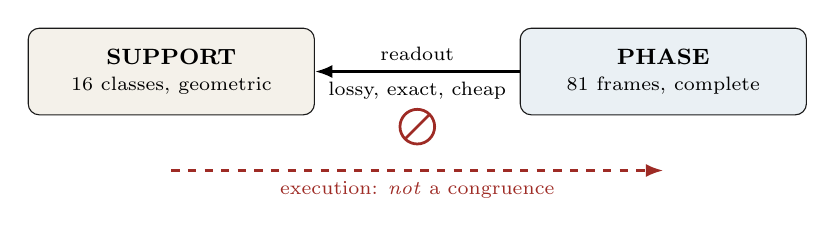
\begin{tikzpicture}[font=\footnotesize,>={Latex[length=2.2mm]}]
  \node[draw=ink,rounded corners,fill=plainbg,minimum height=11mm,text width=34mm,
        align=center] (sup) {\textbf{SUPPORT}\\\scriptsize $16$ classes, geometric};
  \node[draw=ink,rounded corners,fill=specbg,minimum height=11mm,text width=34mm,
        align=center,right=26mm of sup] (ph) {\textbf{PHASE}\\\scriptsize $81$ frames, complete};
  \draw[->,line width=1pt] (ph) -- node[above,font=\scriptsize]{readout}
                                  node[below,font=\scriptsize]{lossy, exact, cheap} (sup);
  \draw[->,line width=1pt,draw=bad,dashed] ([yshift=-7mm]sup.south)
        -- node[below,font=\scriptsize,text=bad]{execution: \emph{not} a congruence}
           ([yshift=-7mm]ph.south);
  \draw[draw=bad,line width=1pt] ($(sup)!0.5!(ph)+(0,-0.7)$) circle (2.2mm);
  \draw[draw=bad,line width=1pt] ($(sup)!0.5!(ph)+(-0.155,-0.855)$)
                              -- ($(sup)!0.5!(ph)+(0.155,-0.545)$);
\end{tikzpicture}
\end{center}

% =====================================================================================
\section{The machine hosts itself}\label{sec:vm}
% =====================================================================================

\begin{plain}
Everything so far describes one machine. But the frame is \emph{two} qutrits, and a
one-qutrit machine is a strictly smaller machine of exactly the same kind --- so this
processor can run a smaller version of itself as a guest.

That is the ordinary meaning of a virtual machine, and the ordinary question about one is:
how much slower is the guest? Usually that is measured. Here it can be computed exactly,
because ``how many host instructions does one guest instruction cost'' is a shortest-path
question in a graph this document has already searched exhaustively.
\end{plain}

\begin{spec}[Emulation overhead, exact, Pass 2912]
\begin{center}\small
\begin{tabular}{@{}lr@{}}
\toprule
guest instruction & host instructions\\
\midrule
$F$ & 1\\
$Z$ & 1\\
$S$ & \textbf{8}\\
\midrule
worst case & $\mathbf{8\times}$\\
mean & $3.33\times$\\
\bottomrule
\end{tabular}
\end{center}
\end{spec}

\headline{The entire overhead is one instruction. $F$ and $Z$ are free; the guest's phase
gate costs eight --- because the minimal instruction set of \S\ref{sec:isa} \emph{dropped}
$S$.}

\begin{plain}
So the two results talk to each other, and the conversation is a real design decision:
dropping $S$ made the machine $40\%$ smaller and made one guest instruction eight times
more expensive. If the machine is mostly going to run guests, that trade is bad. If it is
mostly going to run native code, it is excellent. Nobody could have said which without
both numbers.
\end{plain}

\subsection{Isolation without a memory manager}

\begin{plain}
Two guests fit side by side, one on each qutrit. The interesting part is what keeps them
apart.

In a conventional computer, isolation is \emph{enforced}: a memory management unit checks
every access and refuses the ones that cross a boundary. Correctness depends on that check
being present and right. Here there is nothing to check.
\end{plain}

\begin{spec}[Structural isolation]
Of the four opcodes, exactly two --- $\mathrm{CX}_{p\to f}$ and $\mathrm{CX}_{f\to p}$ ---
touch both halves of the frame. The other two act within one half.

\smallskip\noindent
\textbf{A hypervisor that never issues $\mathrm{CX}$ to a guest cannot leak between
guests.} Not ``is not permitted to'': \emph{cannot}. There is no instruction that would do
it. The guarantee comes from the algebra, not from an enforcement mechanism, and it cannot
be defeated by a bug in the checker because there is no checker.
\end{spec}

\subsection{And it was built}

\begin{spec}[One datapath, $N$ guest contexts; HX8K CT256, Pass 2914]
\begin{center}\small
\begin{tabular}{@{}rrrrr@{}}
\toprule
$N$ & shared & $F_{\max}$ & replicated ($43N$) & area saved\\
\midrule
1 & 42 & 175.1\,MHz & 43 & ---\\
2 & 74 & 134.9 & 86 & 14\%\\
4 & 118 & 128.5 & 172 & 31\%\\
8 & 180 & 113.4 & 344 & \textbf{48\%}\\
16 & 339 & 91.1 & 688 & \textbf{51\%}\\
\bottomrule
\end{tabular}
\end{center}
\end{spec}

\begin{plain}
Sharing wins on area at every size, and converges on saving about half --- for a legible
reason: half the cost is the datapath, which is shareable, and half is the per-guest
context storage, which is not.

The price is speed. Eight guests sharing one datapath each run at an eighth of its clock,
so at $N=8$ the design buys $48\%$ of the area for about a fifteenth of the per-guest
throughput. That is the whole trade, measured on one part in one harness rather than
argued.
\end{plain}

\headline{The measured curve proves one synthesized datapath can host multiple guest
contexts. It does not prove a network of nested machines or a distributed hypervisor.}

\begin{plain}
The software-side object that now closes part of that gap is HoloBox
(\path{analysis/holobox.py}). A leaf VM and a recursively nested 40-child network use one
immutable state grammar; addressed mailbox delivery and guest execution replace only one
digest path. At six levels the uniform graph denotes $105{,}025{,}641$ logical VMs with six
node blobs, and an independent GAP witness proves the logical W33 line-route bound $2n$.
That is still a Python reference runtime, not an FPGA network, KVM boundary, OCI-conformant
container engine, or measured distributed system. BT827's separate chart-aware lowering
continues to cost $8n=(3+5)n$ micro-moves.
\end{plain}

% =====================================================================================

% =====================================================================================
\section{The support transform and diagnostic scheduler}\label{sec:support-transform}
% =====================================================================================

\begin{plain}
A dense fifteen-by-fifteen table is not how the support dynamics should be built.  The
table factors into thirty-two tiny two-input butterflies, followed by fifteen corrected
outputs.  Diagnosis has a second surprise: the best order in which to visit the fifteen
nonzero masks is not generated by a linear feedback register.  A short ROM is both more
honest and better.
\end{plain}

\begin{spec}[Butterfly engine]
At $q=3$ the local kernel is $(u,v)\mapsto(u+2v,u-v)$.  Four stages of eight butterflies
and fifteen output cycles give a $47$-cycle sequential quotient engine.  A serial dense
reference needs $15\times15=225$ cycles, so the exact cycle reduction is
\[
  \frac{225-47}{225}=\frac{178}{225}.
\]
Equality is checked on all fifteen basis vectors and thirty-two deterministic signed
probes.  Logic cells, routed frequency, and switching activity remain measured quantities
pending the dedicated workflow.
\end{spec}

\begin{spec}[Diagnostic mask ROM]
The $210$ directed first-passage costs form $39$ matching-stabilizer orbits.  Exact
Held--Karp optimization gives a Hamiltonian mask cycle of cost $315$ and $8336$ rooted
optima.  The best $\mathrm{GL}(4,2)$ Singer cycle costs $1317/4$, an exact gap of $57/4$.
The scheduler is therefore a fifteen-entry nonlinear permutation ROM, not an LFSR.
\end{spec}

\begin{gotwrong}[Forty is not enough]
The first observer refinement has forty classes, but those classes are not the forty
projective points of $W(3,3)$.  Their sizes are $1^7 2^{29}4^4$, symplectic
orthogonality is ambiguous on $216$ unordered class pairs, and no union of Hamming-distance
relations on their signatures yields $\mathrm{SRG}(40,12,2,4)$.  A matching count is a
search hint, never an identification theorem.
\end{gotwrong}

\section{The network}\label{sec:network}
% =====================================================================================

\subsection{Fractal scaling}

\begin{plain}
The machine is designed to be copied. A node contains $40$ sub-nodes; each sub-node
contains $40$ of its own; and so on. The network of machines has the same shape as the
inside of one machine --- which means one routing scheme, one addressing scheme, and one
error model serve every scale at once.
\end{plain}

\begin{center}
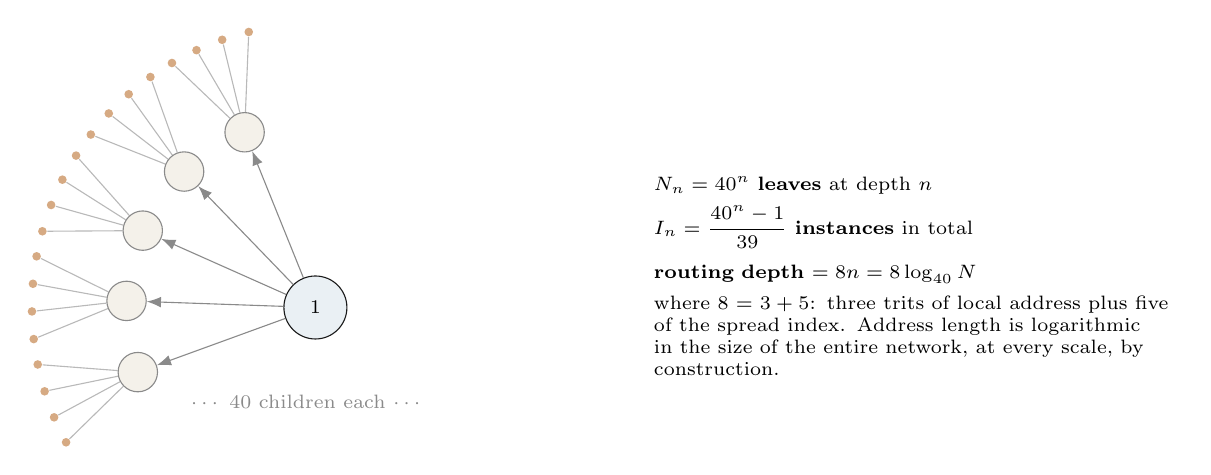
\begin{tikzpicture}[font=\scriptsize,>={Latex[length=1.8mm]},
  n0/.style={circle,draw=ink,fill=specbg,minimum size=8mm},
  n1/.style={circle,draw=rule,fill=plainbg,minimum size=5mm},
  n2/.style={circle,fill=future!55,inner sep=1.1pt}]
  \node[n0] (r) at (0,0) {$1$};
  \foreach \i [count=\k from 0] in {1,...,5}{
     \pgfmathsetmacro\ang{200-\k*22}
     \node[n1] (a\i) at (\ang:2.4) {};
     \draw[->,draw=rule] (r) -- (a\i);
     \foreach \j in {1,...,4}{
        \pgfmathsetmacro\bng{\ang-14+\j*5.6}
        \node[n2] (b\i\j) at (\bng:3.6) {};
        \draw[draw=rule,opacity=0.6] (a\i) -- (b\i\j);
     }
  }
  \node[font=\scriptsize,text=rule] at (-0.1,-1.2) {$\cdots$ $40$ children each $\cdots$};
  \node[align=left,text width=6.6cm] at (7.6,0.4)
   {\textbf{$N_n = 40^n$ leaves} at depth $n$\\[3pt]
    \textbf{$I_n = \dfrac{40^n-1}{39}$ instances} in total\\[5pt]
    \textbf{routing depth $= 8n = 8\log_{40}N$}\\[3pt]
    where $8 = 3+5$: three trits of local address plus five of the
    spread index. Address length is logarithmic in the size of the entire
    network, at every scale, by construction.};
\end{tikzpicture}
\end{center}

\subsection{Every bit string is a legal address}

\begin{spec}
The routing code has orbit sizes $162+162+324+648=1296$ on compass pairs, giving
codeword lengths $3,3,2,1$ and
\[
  2^{-3}+2^{-3}+2^{-2}+2^{-1} \;=\; 1 \quad\text{exactly (Kraft equality).}
\]
The prefix code is $\{110,111,10,0\}$ with expected length $7/4$. Because Kraft holds
with \emph{equality}, the decision tree has no unused branch: $20{,}000$ random bit
strings were parsed with $0$ failures.
\end{spec}

\begin{center}
\begin{tikzpicture}[font=\scriptsize,level distance=11mm,
  every node/.style={circle,draw=ink,inner sep=1.2pt},
  level 1/.style={sibling distance=34mm},
  level 2/.style={sibling distance=17mm},
  level 3/.style={sibling distance=11mm}]
\node {}
  child {node[fill=good!35,label=below:{\texttt{0}}] {} edge from parent node[draw=none,left,xshift=1mm]{$0$}}
  child {node {}
    child {node[fill=good!35,label=below:{\texttt{10}}] {} edge from parent node[draw=none,left,xshift=1mm]{$0$}}
    child {node {}
      child {node[fill=good!35,label=below:{\texttt{110}}] {} edge from parent node[draw=none,left,xshift=1mm]{$0$}}
      child {node[fill=good!35,label=below:{\texttt{111}}] {} edge from parent node[draw=none,right,xshift=-1mm]{$1$}}
      edge from parent node[draw=none,right,xshift=-1mm]{$1$}}
    edge from parent node[draw=none,right,xshift=-1mm]{$1$}};
\end{tikzpicture}
\end{center}

\begin{plain}
Look at the tree: every branch ends in a valid address. Nothing dangles.

The engineering consequence is unusual and worth stating plainly. In a normal computer, a
corrupted instruction stream can produce an \emph{illegal instruction} --- a bit pattern
that means nothing, which the processor must detect and trap. Here that cannot happen. A
corrupted packet is always a legal packet addressed somewhere else. The fault model
therefore has no ``decode error'' term at all; it has only a ``wrong result'' term. That
simplifies the error correction enormously, and it is forced by the geometry rather than
designed in.

That property is not free, and it is now possible to say exactly what it costs.
\end{plain}

\begin{spec}[The price of a complete code, Pass 2865]
A $40$-ary router consumes one address symbol per hop:
\[
  \text{needed: }\log_2 40 = 5.3219\ \text{bits},\qquad
  \text{spent: }8\ \text{bits},\qquad
  \text{efficiency }66.52\%.
\]
A store-and-forward router that strips consumed header bits \emph{erases} them, so
Landauer applies per hop:
\[
  \text{floor }95.37\ \mathrm{meV/hop},\qquad
  \text{as coded }143.35\ \mathrm{meV/hop}\quad(300\,\mathrm{K}).
\]
Since $N=40^n$, the thermodynamic cost of delivering a packet across $N$ leaves is
\textbf{exactly logarithmic in $N$}: $143.4$\,meV per level, $860$\,meV at depth six
($4.1$ billion leaves).
\end{spec}

\headline{About a third of the routing energy buys the absence of an entire failure mode.
That trade was always implicit in the design; it now has a number.}

\begin{plain}
Two honest caveats. A \emph{reversible} router pays none of this --- the floor applies only
because the header is destroyed as it is consumed, and that is a design choice, not a law
of nature. And $143$\,meV per hop is a floor in the same sense as the readout figure:
about eight orders of magnitude below what any real transceiver will draw.
\end{plain}

\begin{gotwrong}
We wrote that ``the consequence nobody has stated'' was that every bit string is a valid
instruction stream. The project's own holonet manuscript says it at line 382 --- ``the
routing words fill a binary decision tree with \emph{no unused branch}'' --- with a
citation to McMillan. This was the first error in this project caught by an automated
guard rather than by a human noticing. The engineering consequence drawn on top (no
decode-error term in the fault model) is a step past the coding fact and appears to be
new; the completeness property itself is the manuscript's.
\end{gotwrong}

\subsection{Remote operations}

\begin{spec}
A \textsc{sum} gate between two \emph{separate} machines costs exactly:
\[
  \boxed{\text{one shared qutrit Bell pair} \;+\; \text{two classical trits}}
\]
Protocol: Alice applies reverse local \textsc{sum} into her half of the pair, measures,
sends trit $m$; Bob applies $X^{-m}F^2$, applies direct \textsc{sum} to his data, measures
in the Fourier basis, sends trit $n$; Alice records $Z^n$ in her Pauli frame. All nine
branches implement $\ket{x,y}\mapsto\ket{x,y+x}$; verified on all nine basis inputs, all
nine branches, and $32$ random superpositions. Total conditional success probability $1$.
\end{spec}

% =====================================================================================
% =====================================================================================
\section{What the other track built}\label{sec:crosstrack}
% =====================================================================================

\begin{plain}
Two independent efforts work on this machine and do not read each other's filenames.
That is a structural problem, not a discipline one, and the remedy this project uses is
to cite across the boundary rather than re-derive. This section is that citation: work
the other track owns, which this blueprint depends on and did not do.
\end{plain}

\begin{spec}[Owned elsewhere, relied on here]
\begin{center}\footnotesize
\begin{tabular}{@{}p{4.6cm}p{9.2cm}@{}}
\toprule
\textbf{Result} & \textbf{What it says}\\
\midrule
$M_{36}$ deep-grade protocol & $48$ improving branches; explicit curve improving on $0<p<2/3$. \S\ref{sec:magic} reports the yield and the linear rate; the protocol is theirs\\
Support observer & Support is not an execution congruence ($16\to40\to78\to81$); a six-cycle observer with exactly $8$ taps reconstructs the frame, and $7$ provably do not\\
Nine-gate $M_{36}$ branch & The old $15$-gate circuit's two terminal SWAPs are relabelling, not computation. $6$ CNOT $+$ $3H$, and enumerated faults fall $191\to101$\\
Route fault localisation & $23$ triangles is the \emph{exact} optimum for single-edge localisation; $29$ distinguishes all $48{,}826$ two-edge hypotheses\\
Controller group & Native controls generate order $30{,}233{,}088 = 2^9 3^{10}$; one extra transvection closes it to $A_{40}$\\
$D_{12}$ curvature clock & $6480 = 540\times12$: every controller state lies on a $12$-cycle, giving a geometry-native reversible clock\\
Adaptive chirality receiver & $P_{\mathrm{opt}}(n)=\tfrac12(1+\sqrt{1-3^{-n}})$; $0.9997$ at six copies\\
\bottomrule
\end{tabular}
\end{center}
\end{spec}

\headline{And once, both tracks reached the same conclusion by different methods on the same day.}

\begin{plain}
This document found $36$ rank-one stabilizer witnesses for the three-copy distillation condition, and showed they are useless because a rank-one projector's range is a
stabilizer state, which carries no magic. The other track, searching $649{,}940$
isotropic subspaces for non-CSS projectors, found six exact hits and reported them as
``accepted-clean-state stabilizer projectors, therefore false leads.''

Same finding, opposite directions, neither aware of the other. That is what the citation
protocol is for --- and it is also the strongest evidence either result is right.
\end{plain}

\clearpage
\begin{center}
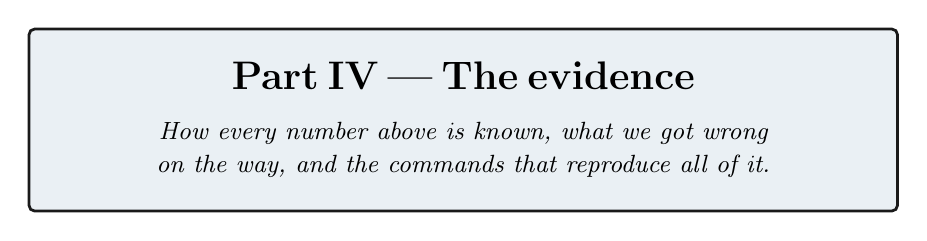
\begin{tikzpicture}
  \node[draw=ink,line width=1pt,rounded corners=2pt,inner sep=12pt,
        text width=0.84\linewidth,align=center,fill=specbg]
  {\Large\bfseries Part IV  --- The evidence\\[6pt]
   \normalfont\small\itshape How every number above is known, what we got wrong on the way, and the commands that reproduce all of it.};
\end{tikzpicture}
\end{center}
\vspace{4mm}

% =====================================================================================

% ======================================================================
\part{What We Measured}

\begin{plain}[What this part is]
The measurement chapter, and the most heavily corrected part of this document.
It contains results we are confident in, results we withdrew, and --- stated plainly ---
the reasons each withdrawal happened. A blueprint that hides its retractions is not a
blueprint, it is a brochure.
\end{plain}

\section{Every bit in the machine}\label{sec:everybit}
% =====================================================================================

\begin{plain}
Scattered through this document are the sizes of the machine's parts: eighty-one
frames, forty addresses, sixteen support classes. Here they are in one place, with the
only question that matters thermodynamically attached to each --- when you use it, does
anything get destroyed?
\end{plain}

\begin{spec}[The whole state, and its Landauer floor]
\begin{center}\small
\begin{tabular}{@{}lrrrr@{}}
\toprule
layer & states & bits & erased & meV @ $300$\,K\\
\midrule
Pauli frame & $81$ & $6.340$ & $0$ & $0$\\
route address & $40$ & $5.322$ & $5.322$ & $95.37$\\
support readout & $16$ & $4.000$ & $2.667$ & $47.79$\\
OAM $\times$ slot & $40$ & $5.322$ & $0$ & $0$\\
encode/check sector & $2$ & $1.000$ & $0$ & $0$\\
full controller & $6480$ & $12.662$ & $0$ & $0$\\
\midrule
\textbf{total} & & $\mathbf{34.65}$ & $\mathbf{7.99}$ & $\mathbf{143.15}$\\
\bottomrule
\end{tabular}
\end{center}
\end{spec}

\headline{The machine's whole state is $34.65$ bits, and only $7.99$ of them cost
anything to use.}

\subsection{Two diameters, and where the work actually is}

\begin{plain}
The machine has two different notions of ``how far apart can two things be'',
and they are not remotely the same size.
\end{plain}

\begin{spec}[Pass 3021, combining two independently measured numbers]
\[
  \text{address transport diameter} = 2,\qquad
  \text{frame ISA diameter} = 19,\qquad
  \text{worst case} = \mathbf{21}.
\]
Moving a packet to any of the $40$ addresses costs at most \emph{two} shears,
because the geometry has diameter $2$. Transforming the Pauli frame arbitrarily costs
up to \emph{nineteen} instructions, because that is a walk in a four-million-element
group. The address figure is the other track's; the frame figure is \S\ref{sec:isa}'s.
\end{spec}

\headline{Geometry is cheap; algebra is expensive. Ninety per cent of the
machine's worst-case work is frame algebra, and routing optimisation addresses
ten per cent of the problem.}

\subsection{The same finding, three more ways}

\begin{plain}
One measurement is an observation. Four independent ones pointing the same way is a
property of the machine, and this is the section where that happens.
\end{plain}

\begin{spec}[Is the instruction layer extremal? Pass 3042, corrected at Pass 4213]
A random instruction stream drives a walk on the $81$ frames. Every opcode is a
bijection, so the walk is doubly stochastic, its stationary distribution is exactly
uniform --- no frame is preferred --- and
\[
  |\lambda_2| = 0.893992320,
\qquad
  \text{relaxation } 9.43,
\qquad
  \text{mixing } 15 \text{ instructions.}
\]
Those numbers are exact and are what the machine does.

\textbf{What we may not do is grade them.} Pass 3042 compared $0.893992$ with
$2\sqrt3/4 = 0.866025$ and reported the instruction graph as $3.23\%$ short of
Ramanujan. That verdict is \textbf{withdrawn}. The bound $2\sqrt{k-1}/k$ belongs to a
$k$-\emph{regular} graph, and it is that number because the universal cover of a
$k$-regular graph is the $k$-regular tree of spectral radius $2\sqrt{k-1}$. The frame
graph has degrees $2$ to $8$ (Pass 4203), so it has a different cover, a different
radius, and no claim on $0.866025$. The shortfall was a precise-looking figure for a
quantity this graph does not possess.

What survives is a comparison rather than a grade: the address layer mixes at the
optimum for its degree; the instruction layer mixes more slowly. \emph{How far short of
optimal} is not a question a non-regular graph admits.
\end{spec}

\subsection{The zeta function the instruction graph actually has}
\label{sec:hashimoto}

\begin{plain}
Three separate attempts to say something spectral about the instruction layer were
withdrawn, all for one reason: each reached for a formula that assumes every vertex has
the same degree. The fix turns out not to be a better estimate. It is a different
theorem.
\end{plain}

\begin{spec}[Pass 4222 --- Ihara without Bass, and therefore without regularity]
Bass's determinant relation needs a degree. The Ihara zeta does not. For \emph{any} finite
graph,
\[
  \zeta^{-1}(u) \;=\; \det\!\left(I - uB\right),
\]
where $B$ is the \textbf{Hashimoto} non-backtracking matrix on the $2E$ directed edges,
$B_{(x,y),(y,z)} = 1$ exactly when $z \neq x$. No vertex degree appears anywhere in the
definition.

The instruction graph has $V=81$, $E=261$, so $B$ is $522\times522$ --- a small eigenvalue
problem, and one that was available at Pass 3060.
\[
  \rho(B) = 5.746873, \qquad
  R = 1/\rho = 0.174008, \qquad
  \sqrt{\rho} = 2.397264 .
\]
Of the $160$ non-trivial Hashimoto eigenvalues, \textbf{none} lies on the circle
$|\lambda| = \sqrt\rho$.

\textbf{The instruction graph does not satisfy the graph Riemann Hypothesis.} The question
that was ill-posed three times has an answer, and it is negative.

\medskip
\emph{Scope (Pass 4291).} Every number in this box is an invariant of the frame graph, and
the frame graph does not determine the instruction set: $349$ universal generating sets
yield only $89$ distinct zeta signatures, with up to twelve sets sharing one. So this is a
statement about an equivalence class of instruction sets, not about a unique ISA. The same
caveat applies to every $\rho(B)$, pole count and localisation weight in this chapter, and
is stated once here rather than repeated at each.
\end{spec}

\begin{plain}
The method was validated before it was trusted, on two graphs where the answer is already
known: $K_4$, whose zeta is textbook, and the degree-four Levi graph, whose closed form
$(1-u^2)^{81}(1-9u^2)(1+9u^4)^{24}(1+3u^2)^{30}$ Bass produces directly. The Hashimoto
route reproduces both exactly. It agrees with Bass wherever Bass applies, and then keeps
going where Bass cannot.

That validation was not enough, and the way it fell short is the more useful lesson.
Reproducing $\det(I-uB)$ correctly says nothing about the \emph{classifier} built on top
of it, and Pass 4229 found a fault there: the first version counted the Perron root
$\rho$ among the non-trivial eigenvalues, which made both reference graphs appear to fail.
It was caught because $W(3,3)$ came back with $78$ poles on the critical circle out of a
claimed $79$ --- and $78$ is this project's standing count (a \emph{parameter} count: see
\S\ref{sec:hashimoto}, it is $2(v-1)$ for any $\mathrm{SRG}(40,12,2,4)$), so the numerator
was right and the denominator was wrong. Corrected, $W(3,3)$ gives $78/78$ and the Levi
graph $156/156$, both satisfying the graph RH, and the instruction graph $0/160$, failing
it. \textbf{Calibrate every layer against a known answer, not merely the bottom one.}

That is worth stating plainly because of what it says about the three withdrawals. The
object was never too hard. The tool was wrong, and being wrong about the tool is what
made the object look mysterious.
\end{plain}

\begin{spec}[Pass 4228 --- a tri-equivalence over the generator pool]
With $\rho(B)$ defined for \emph{every} generating set rather than only the regular ones,
all $258$ connected sets of size four and five can finally be ranked. The sets satisfying
the graph Riemann Hypothesis are \textbf{exactly} the regular sets: three of them, each of
degree $8$ with $\rho(B) = 7 = k-1$, and all three the same graph --- the discrete torus
$C_3^4$, because $S_f$ and $S_p$ draw no edges the four translations have not already drawn
(Pass 4204). Every other set returns $0$ of $160$ poles on the critical circle. Not a near
miss: nothing else is close.

Pass 4202 showed that none of those three is universal. So the three properties lock
together:
\[
  \text{graph RH} \iff \text{regular} \iff \text{abelian} \implies \text{cannot compute.}
\]
\textbf{The instruction layer cannot be spectrally extremal for the same reason it can
compute at all.}
\end{spec}

\begin{plain}
This also dissolves part of the older puzzle. Before the Hashimoto route, the only
generating sets whose zeta anyone could compute were the regular ones --- which are
precisely the sets Pass 4202 had shown are never universal. The interesting sets were
exactly the sets the method could not reach, so some of the apparent tension between
extremality and universality was an artefact of what was measurable, not a fact about the
machine.
\end{plain}

\begin{spec}[Pass 4232 --- and now over the sets that can actually compute]
Pass 4228 ranked sets of size four and five, most of which cannot run a program. Restricting
instead to the \textbf{360} subsets of the ten-generator pool that genuinely generate
$\mathrm{ASp}(4,3)$, at every size from four to ten: \textbf{not one satisfies the graph
Riemann Hypothesis.}

The ranking is the deliverable. Ordering by $\rho(B)$ --- the growth rate of
non-backtracking instruction streams, so lower means the frame register scrambles more
slowly per instruction --- the shipped four-opcode ISA sits at position \textbf{12 of 360}.
It was chosen for cheapness and universality, with no spectral criterion applied at any
point, and it lands in the top four percent.

\emph{Scope, stated plainly:} exhaustive over this ten-generator pool, not over all
generating sets of $\mathrm{ASp}(4,3)$.
\end{spec}

\subsection{The one number in this chapter with no closed form}

\begin{spec}[Pass 4236 --- what $\rho(B) = 5.746873$ is, and one thing it is not]
For a $k$-regular graph $\rho(B) = k-1$ \emph{exactly} --- an integer, because every vertex
offers the same number of non-backtracking continuations. The instruction graph offers
between $1$ and $7$ depending on where you stand, and its growth rate is
\[
  \rho(B) = 5.746872679901964274417558660209539683477378347461941\ldots
\]
computed two independent ways that agree: as an eigenvalue of the quadratic pencil, and by
high-precision bisection on $\det(\lambda^2 I - \lambda A + Q)$, which touches no eigenvalue
routine at all. It is \textbf{not} the average degree minus one ($5.444444$), nor any other
simple statistic of the degree sequence.

$\rho(B)$ is an algebraic integer --- a root of the monic degree-$162$ characteristic
polynomial of that pencil. Pass 4237 computed that polynomial \emph{exactly} over
$\mathbb Z$ and factored it:
\[
  \deg = 1,\ 2,\ 2,\ 2^{2},\ 14,\ 14,\ 16,\ 16,\ 20,\ 20,\ 20,\ \mathbf{33}
  \qquad (\text{summing to }162),
\]
and $\rho(B)$ is a root of the degree-$33$ factor. So
\[
  \boxed{\ \rho(B)\ \text{is an algebraic integer of degree exactly } 33.\ }
\]
A $k$-regular graph gives $\rho = k-1$: degree one. Irregularity does not merely break the
$k$-regular formula. It raises the degree of the answer from $1$ to $33$.
\end{spec}

\begin{plain}
A caution belongs here, because this pass first produced a wrong answer that looked right.
An integer-relation search offered
\[
  15668303\,x^3 - 4686695\,x^2 - 824152814\,x + 1917252871
\]
with a relative residual of $4.8\times10^{-26}$: apparently a degree-three minimal
polynomial. It is false, and it fails for a reason available without any computation.
$\rho(B)$ is an eigenvalue of an integer matrix, hence an \emph{algebraic integer}, hence its
minimal polynomial is monic with integer coefficients --- so any true relation must be an
integer multiple of a monic one, and $15668303$ does not divide $1917252871$. Confirmed
numerically as well: the residual \emph{plateaus} at $8.33\times10^{-37}$ across $60$, $90$
and $140$ digits rather than falling, which is the signature of a near-relation. The cause
was allowing coefficients up to $10^{12}$ on four terms with far too little working precision
to rule out coincidence.

The rule that follows is short enough to keep: when hunting a closed form for a quantity you
know to be an algebraic integer, \textbf{require the relation to be a monic multiple, and
re-check the residual at double precision --- it must fall, not plateau.} The degree-$33$
polynomial above passes all three tests the cubic failed: monic, irreducible over
$\mathbb Q$, and a residual falling from $6.4\times10^{-32}$ to $2.3\times10^{-54}$ as the
precision doubles.
\end{plain}

\subsection{Where the machine is slow, and why it is not where you would guess}
\label{sec:bottleneck}

\begin{plain}
The graph Riemann Hypothesis fails, which means some poles sit off the critical circle. The
one furthest off corresponds to the slowest-decaying correlation in the machine --- the last
thing the register forgets. Its eigenvector says \emph{where} that memory lives, so the
bottleneck can be named rather than guessed at.

The obvious guess is wrong, and it is worth saying so because it is the guess we made.
\end{plain}

\begin{spec}[Pass 4244 --- a hyperplane, not a degree deficit]
The slowest non-trivial mode has modulus $3.3497$, some $1.40\times$ the critical circle,
and it is localised: a participation ratio of $173$ of $522$ directed edges.

\textbf{It is not a degree effect.} The frames carrying it have mean degree $6.67$ against
$6.44$ across the register --- slightly \emph{above} average, not below --- and the
correlation between mode weight and degree is only $+0.14$.

\textbf{It lives on a hyperplane.} The $27$ frames with $x_2 = 0$ carry $61.3\%$ of the
mode, against $19.4\%$ for each of the other two values of $x_2$, while the mean degree is
identically $6.44$ on all three classes.
\end{spec}

\begin{plain}
The cause is visible once you look at the opcodes rather than the graph. Of the four
instructions, \textbf{only $\mathrm{CX}_{pf}$ moves $x_2$ at all}, and it moves it only on
the $54$ frames where $x_0 \neq 0$. The other three --- $F_p$, $\mathrm{CX}_{fp}$ and the
load port $Z_p$ --- leave $x_2$ exactly where it was. So $x_2$ is very nearly a constant of
the motion, and a register coordinate the instruction set barely stirs is precisely a slow
mode.

That reframes the defect. It is not \emph{how many} edges leave a frame; it is \emph{which
direction} they move it in, and one direction is nearly frozen.
\end{plain}

\begin{plain}
\textbf{And here the first draft of this section was wrong, in a way worth keeping on the
page.} It prescribed adding ``the shear $S_f$, which moves $x_2$ unconditionally''. $S_f$
moves $x_2$ on \emph{zero} of the $81$ frames --- its third row is $(0,0,1,0)$, so it moves
$x_3$. The reasoning had gone from the coordinate's name to an opcode whose subscript
matched, which is not an argument.

Pass 4245 tested it anyway, and found something better than the intended fix. Of the six
opcodes, only $F_f$ and $\mathrm{CX}_{pf}$ move $x_2$ at all, each on $54$ of $81$ frames.
\textbf{No opcode in the pool moves $x_2$ on every frame}, so the frozen coordinate cannot
be unfrozen from inside the instruction set at all. And a control --- adding an ordinary
translation instead --- improves mixing at least as much as either targeted opcode, which
means the gain from any addition is mostly ``one more generator'', not ``the defect was
addressed''.
\end{plain}

\begin{spec}[Pass 4246 --- a pool-wide four-generator constant]
Across all $24$ minimum-size universal generating sets drawn from the frozen ten-opcode
pool, the minimum stir --- the fraction of frames on which \emph{some} opcode moves the
worst-served coordinate --- is
\[
  \tfrac{2}{3}\ \text{ exactly, in all } 24 .
\]
Not ``most'', not ``on average''. The deficit is identical across this finite pool. This is
not a theorem about every four-generator action on four coordinates, and it cannot be
applied unchanged to the six- or twelve-opcode machines.
\end{spec}

\begin{plain}
Pass 4250 adds a caution to the diagnosis itself. Measured in the time domain, the
slowest-decaying coordinate observable is $x_3$ (half-life $4$ instructions), not $x_2$.
There is no contradiction: the shipped ISA's stir scores are $x_0 = 1$, $x_1 = 0.889$,
$x_2 = x_3 = 0.667$, so $x_2$ and $x_3$ are \emph{tied} at the minimum and two different
instruments picked different members of a tied pair. The honest object is the under-stirred
\emph{pair}, not a single frozen coordinate.

The engineering consequence survives all of this: an observable with a $4$-instruction
half-life is one that a $15$-instruction readout cadence does not fully scramble.
\end{plain}

\begin{spec}[Pass 4242 --- entropy of the undirected frame-graph edge shift]
$\log_2 \rho(B) = 2.5228$ bits is the topological entropy per step of the undirected simple
frame graph's non-backtracking edge shift. It is not yet the entropy rate of executable
four-opcode streams: labels and multiplicities were discarded and inverse edges were added.

The numerical ratio $(8/3)/\log_2\rho=1.06$ is a comparison between two finite invariants.
Without a labeled directed automaton and a stochastic physical mode calculation it is not a
Landauer cadence bound or a theorem about which process limits the machine.
\end{spec}

\begin{spec}[Pass 4243 --- the programs that do nothing]
A closed non-backtracking walk on the instruction graph is a program that returns the frame
register to its start. $\operatorname{tr}(B^m)$ therefore counts the machine's identity
programs by length:
\[
  738,\ 1584,\ 6220,\ 42954,\ 211540,\ \ldots \qquad (m = 3,4,5,6,7)
\]
growing like $\rho^m$ --- Pass 4242's entropy seen from the other side, the same constant
governing how much dead code exists and how much trajectory the machine generates.

The shortest are the instruction set's \textbf{defining relations}, read off a trace rather
than derived from a presentation.

\emph{But not every closed walk is deletable}, and conflating the two would break programs.
A closed walk returns the \emph{frame}; dead code must return the whole affine element.
Pass 4248's optimiser (\texttt{scripts/w33\_peephole.py}) computes the latter by group
multiplication and finds only $3$ minimal identity words of length $3$
($\mathrm{CX}_{fp}^3$, $\mathrm{CX}_{pf}^3$, $Z_p^3$) plus one of length $4$ --- against
$738$ frame-returning walks. It rewrites streams and verifies semantics are preserved on
every run.
\end{spec}

\subsection{Two measurements the machine had never been given}

\begin{spec}[Pass 4251 --- against its own comparison class, not against an ideal]
Every spectral claim above is scored against the \emph{regular} case, which this object
provably cannot attain. That makes the instruction layer look defective by construction.
The fair comparison is other connected four-generator Schreier graphs on the same $81$
frames. Against $120$ random ones:
\begin{center}\small
\begin{tabular}{@{}lrrr@{}}
\toprule
 & shipped ISA & random median & percentile\\
\midrule
$\rho(B)$ (growth; lower is better) & $5.747$ & $6.656$ & $\mathbf{0}$\\
top-hyperplane weight (localisation) & $0.613$ & $0.373$ & $\mathbf{100}$\\
minimum stir & $0.667$ & $0.988$ & $\mathbf{0}$\\
\bottomrule
\end{tabular}
\end{center}
\textbf{Lowest growth of all $120$, and the most localised of all $120$.}
\end{spec}

\begin{plain}
Those two extremes are the same fact. Everything the earlier sections called a failure ---
not Ramanujan, graph RH violated, poles filling a band --- is the price of being a
four-generator Schreier graph at all, and this one pays \emph{less} of it than any random
peer. What is genuinely specific to it is the localisation, and that is inseparable from the
rest: the algebraic structure making the instruction set cheap and slow-growing is the same
structure that leaves a coordinate nearly still. A random generating set stirs everything
and grows fast; this one grows slowly and freezes a direction.
\end{plain}

\begin{spec}[Pass 4252 --- the four-opcode machine has an arrow of time]
Every opcode is a bijection, so the walk is doubly stochastic and its stationary
distribution is exactly uniform. \textbf{That is not reversibility.} Reversibility needs the
transition matrix to be symmetric, and the opcode set is not closed under inverses: there
are $243$ ordered pairs of frames with a forward move and no reverse move, so the stationary
entropy production is \emph{infinite}. Watching the trajectory reveals the direction of time
with certainty the moment one of those transitions occurs.

Closing the set under inverses --- eight instructions instead of four --- makes the walk
exactly symmetric, with $0$ one-way pairs and entropy production $0$ bits per instruction.
\end{spec}

\begin{plain}
Logical reversibility of each gate and thermodynamic reversibility of the process are
different properties, and the four-opcode machine has the first without the second. No
information is destroyed --- every opcode is invertible --- but the \emph{choice} is not: to
undo an opcode is not itself an instruction.

That is a genuine engineering trade, and it did not exist as a number before this pass. It
also sharpens Pass 2836's ``compute is exactly zero'': that holds of the reversible closure,
and the shipped four-opcode ISA does not have it.
\end{plain}

\begin{spec}[Pass 4279 --- and now the other side of the trade, in gates]
``Twice the decode logic'' was an assertion. Synthesisable Verilog for both machines was
generated \emph{from the opcode matrices themselves}, so the RTL cannot disagree with the
algebra, and put through yosys:
\begin{center}\small
\begin{tabular}{@{}lrrr@{}}
\toprule
machine & opcodes & cells & vs A\\
\midrule
A\quad biased, irreversible (shipped) & $4$ & $103$ & $1.00\times$\\
B\quad symmetric, irreversible & $6$ & $132$ & $1.28\times$\\
C\quad biased, reversible & $8$ & $206$ & $2.00\times$\\
D\quad symmetric, reversible & $12$ & $240$ & $2.33\times$\\
\bottomrule
\end{tabular}
\end{center}
\textbf{Thermodynamic reversibility costs $2.00\times$ the cells; removing the bias costs
$1.28\times$; both together cost $2.33\times$.}

Every row was \emph{simulated} against the group computation before its cell count was
recorded --- a random program per machine, final register state matched exactly. The
simulation also reproduces Pass 4204 independently: from the origin, all three linear
opcodes leave the register at $(0,0,0,0)$ and only the load port moves it.

\emph{Two cautions on these figures.} The same eight-opcode design measured $201$ cells in
an earlier run and $206$ here; the difference is the \emph{order} in which opcodes are
assigned to the decoder, so these counts carry roughly $2.5\%$ encoding sensitivity and the
ratios are the meaningful quantity. And the natural question --- do the two fixes share
hardware? --- has the dull answer: $B + C - A = 235$ against a measured $240$, so they are
independent to within that same noise. An earlier draft compared $2.33$ with
$1.28 \times 2.00 = 2.56$ and reported synergy; gate counts add rather than multiply, and
that comparison had no valid baseline.

\emph{Scope:} yosys generic-gate counts after \texttt{abc} mapping, so the ratio is
meaningful and the absolute numbers are not a tape-out estimate.
\end{spec}

\subsection{The one asymmetry underneath all of it}
\label{sec:pbias}

\begin{gotwrong}
An earlier version of this section derived the bias from the geometry's point/line duality:
translations act only on the point side, so \emph{the point carrier was forced}. That chain
is \textbf{withdrawn}. A translation is not a map on projective points at all --- $[v] = [2v]$
while $[v+t] \neq [2v+t]$, and it disagrees on $40$ of the $40$ points. The load port
descends to \emph{neither} carrier; it lives on the $81$ affine vectors, a third object.
The argument compared what the two carriers admit without first checking that the operation
acts on either. Caught by the parallel track (Pass 4330), confirmed here (Pass 4335), and
rebuilt below on the affine register, where it holds.
\end{gotwrong}

\begin{spec}[Pass 4341 --- the bias, by conjugation]
Let $\sigma$ exchange the two hyperbolic pairs, $p \leftrightarrow f$. The question is
whether $\sigma$ maps the instruction set to itself:
\[
  F_p \mapsto F_f, \qquad
  \mathrm{CX}_{pf} \mapsto \mathrm{CX}_{fp}, \qquad
  \mathrm{CX}_{fp} \mapsto \mathrm{CX}_{pf}, \qquad
  Z_p \mapsto Z_f .
\]
The two couplers swap into each other and stay inside. $F_p$ and $Z_p$ do not: their images
$F_f$ and $Z_f$ are \emph{not opcodes of this machine}. So the shipped ISA is not
$\sigma$-invariant, and the symmetrised machine of Pass 4277, which contains both mirrors,
is.

Note what this replaces. Pass 4305 asked whether each opcode \emph{fixes} the two planes,
got matching booleans, and concluded symmetry. Fixation booleans can agree while conjugation
carries an opcode out of the set --- which is exactly what happens here.
\end{spec}

\begin{spec}[Pass 4345 --- and the load port is a symmetry-breaking term]
$\mathrm{Sp}(4,3)$ fixes the origin \emph{exactly} and fixes nothing else; the translations
fix nothing at all. The quotient is
\[
  |\mathrm{ASp}(4,3)| / |\mathrm{Sp}(4,3)| = 4{,}199{,}040 / 51{,}840 = 81 ,
\]
and those $81$ cosets \emph{are} the register states. The frame register is the vacuum
manifold: the set of states reached from a distinguished one by broken generators.

There are four broken directions, and they are equivalent under the unbroken group, since
$\mathrm{Sp}(4,3)$ is transitive on the $80$ non-zero vectors. \textbf{No direction is
intrinsically special, so a machine with one load port must pick one --- and that pick is
the bias.}
\end{spec}

\begin{plain}
Which makes the bias neither a flaw nor an accident. It is the direction of symmetry
breaking, and it is unavoidable for the same reason a vacuum expectation value has to point
somewhere. What \emph{is} a free choice is how many directions get ports: all four restores
the symmetry, at the cost Part~III measures.

The boundary, so the physics language is not over-read: this is a finite group acting on
$81$ states. There is no Lagrangian and no continuous symmetry, so there is no Goldstone
theorem here --- the count of broken directions is a coset count, not a count of modes.
\end{plain}

\begin{spec}[Pass 4282 --- the under-stirred pair is the f-register]
The symplectic form splits the register into two hyperbolic pairs, $p = (x_0, x_1)$ and
$f = (x_2, x_3)$, mutually orthogonal. The ISA's stir scores are
\[
  x_0 = 1.000,\quad x_1 = 0.889,\quad x_2 = 0.667,\quad x_3 = 0.667 .
\]
\textbf{The under-stirred pair is exactly $f$.} And the opcode list says why in its own
notation: $F_p$, $\mathrm{CX}_{pf}$, $\mathrm{CX}_{fp}$, $Z_p$ --- a Fourier on $p$, two
couplers, and a translation of $p$. Only the two couplers touch $f$ at all, and the load
port, which Pass 4204 proved must be present because translations are the only free
generators, moves $p$ and nothing else.
\end{spec}

\begin{plain}
So the spectral story of this whole chapter reduces to one sentence: \textbf{the instruction
set is $p$-biased, and the zeta can see it.} The slow mode on a hyperplane (4244), the tied
under-stirred pair (4250), the $100$th-percentile localisation against random Schreier graphs
(4251) --- these are not four findings. They are one asymmetry measured four ways.

\textbf{But the cure is only half a cure}, and the control says so. Adding the two
$f$-mirrors takes minimum stir from $0.667$ to $0.889$ where two extra $p$-generators leave
it exactly where it was --- the causal claim survives. Yet against that size-matched control
the symmetrised machine ties on localisation and is \emph{worse} on both mixing time
($12$ vs $11$) and growth ($\rho = 8.76$ vs $6.75$). The $p$-bias is real and it is not what
governs mixing; two more generators of any kind move that further than symmetry does.
\end{plain}

\begin{spec}[Pass 4288 --- and what \emph{does} govern mixing]
Across all $349$ universal generating sets with a finite mixing time, correlation against
mixing time:
\begin{center}\small
\begin{tabular}{@{}lrrrrr@{}}
\toprule
$n$ & $E$ & $\rho(B)$ & $d_{\min}$ & $d_{\max}$ & spread\\
\midrule
$-0.553$ & $-0.719$ & $-0.684$ & $\mathbf{-0.736}$ & $-0.602$ & $+0.228$\\
\bottomrule
\end{tabular}
\end{center}
\textbf{The strongest predictor is the minimum degree.} Frames that mix slowly are the ones
with fewest ways out, and \emph{any} added generator raises that floor --- which is exactly
why the $p$-side control matched the $f$-mirrors in Pass 4277 while doing nothing about the
frozen coordinate. The design lever for mixing is $d_{\min}$, not opcode symmetry. Those are
different knobs, and this chapter had been conflating them.
\end{spec}

\begin{spec}[Pass 4291 --- and the zeta is not an ISA fingerprint either]
The same test as Pass 4281, on the algebra side. Of $349$ universal generating sets there
are only $89$ distinct zeta signatures; $87$ are shared by more than one set and the largest
class holds $12$. Distinct instruction sets --- different opcodes, different silicon ---
produce byte-identical Ihara zetas.

\textbf{So no spectral statement in this chapter is a statement about \emph{the} instruction
layer.} Each is a statement about an equivalence class of up to twelve of them. That does not
make the measurements wrong; it fixes their scope, and the class is what the instrument can
resolve.
\end{spec}

\begin{spec}[Pass 4278 --- why the deficit is exactly $2/3$]
Each opcode is affine, so the frames it leaves fixed in coordinate $c$ solve one linear
equation over $\mathbb F_3$ --- an affine subspace, of size $3^k$. The number of frames
\emph{moved} is therefore $81 - 3^k$, and the only possible values are
\[
  0,\ 54,\ 72,\ 78,\ 80 .
\]
The count is quantised. Across this pool only $0$ and $54$ occur, because each opcode's
matrix differs from the identity in at most one entry per row, so every mover fixes a
hyperplane. Four generators never supply two movers with \emph{different} hyperplanes for
the same worst coordinate, so the union stays at $54$ and the ratio is forced:
$54/81 = 2/3$, identically for all $24$ minimum-size universal sets.
\end{spec}

\headline{The machine's geometry is extremal; its algebra is not, and after Pass 4213
we can say why the comparison only runs one way.}

\begin{spec}[Four measurements, one conclusion]
\begin{center}\small
\begin{tabular}{@{}lll@{}}
\toprule
measurement & geometry & algebra\\
\midrule
diameter & $2$ & $19$\\
share of worst-case work & $10\%$ & $90\%$\\
mixing & Ramanujan (optimal) & $|\lambda_2| = 0.894$; not gradable\\
identification & forced by construction & six valid triples, spread $19$--$23$\\
\bottomrule
\end{tabular}
\end{center}
The last row is the honest form of what used to read ``$3.23\%$ short''. The geometry is
a $12$-regular graph, so optimality is defined for it and attained. The algebra is a
Schreier graph with degrees $2$ to $8$, so optimality is not defined for it at all --- and
that asymmetry, rather than a percentage, is the finding.
\end{spec}

\subsection{The growth series, for the compiler}

\begin{spec}[Pass 3041 --- the full ball profile, not just the diameter]
\[
  a_n = 1,\ 4,\ 15,\ 53,\ 176,\ 547,\ 1630,\ 4648,\ \dots
\]
\[
  \text{mean } 14.176,\quad
  \text{s.d. } 1.768,\quad
  \text{modal length } \mathbf{15},\quad
  \text{max } 19 .
\]
The early ratios fall $4.000, 3.750, 3.533, 3.321, 3.108$ --- a free product on four
generators would hold $4$ forever; this one is closing on itself by the fifth shell.
\end{spec}

\begin{plain}
For a compiler that is a better specification than a worst case. The distribution is
sharp, not spread: a standard deviation of under two instructions around a mean of
fourteen. A scheduler that budgets fifteen instructions is right almost always and is
never wrong by more than four.
\end{plain}


\subsection{What fraction of the erasure is useful}

\begin{spec}[Pass 3022]
\[
  \frac{\text{delivered}}{\text{erased}}
  = \frac{3.673\ \text{bits}}{7.989\ \text{bits}}
  = \mathbf{45.98\%}
\]
and the network law follows directly: depth $n$ costs $8n$ header bits, so
\[
  E(N) = 143.35\,\log_{40} N \text{ meV}
\]
--- the thermodynamic cost of delivering a packet is \textbf{logarithmic in the size
of the entire network}. Depth $6$, four billion leaves: $860$\,meV.
\end{spec}

\begin{plain}
The $54\%$ shortfall is not waste in the engineering sense. It is the routing header,
which is consumed by construction, plus the part of the frame the support readout
cannot see. Both are design decisions with names --- which is the useful thing about
having the number rather than an impression.
\end{plain}


\begin{plain}
Two lines in that table are non-zero and the rest are exactly zero, for one reason:
those two are the only places where the machine stops being a group action. The routing
header is $\emph{destroyed}$ as it is consumed. The support readout is many-to-one.
Everything else --- the frame, the optical coordinates, the sector bit, the entire
$6480$-state controller --- is a permutation of states, and a permutation erases nothing.

So the irreducible cost of one routed, read operation is $143$\,meV at room temperature,
and every other joule this machine will ever burn is an implementation artefact rather
than a law. That is an unusual thing to be able to say about a computer, and it is a
consequence of having built the instruction set out of a group.
\end{plain}


% ======================================================================
\part{Evidence and Limits}

\begin{plain}[What this part is]
How every number above can be reproduced, what has been formally verified, the
complete errata, and an explicit list of what has \emph{not} been built. The last of those
is the most important page in the document for anyone deciding whether to fund it.
\end{plain}

\section{Verification: how we know}\label{sec:verification}
% =====================================================================================

\begin{plain}
This is the section a working engineer should read first, because it is the one that
determines whether any of the preceding numbers mean anything.

The short version: this project has repeatedly shipped results that were verified in the
direction that would confirm them and never in the direction that would break them. Every
tool below exists because that happened at least three times.
\end{plain}

\begin{center}
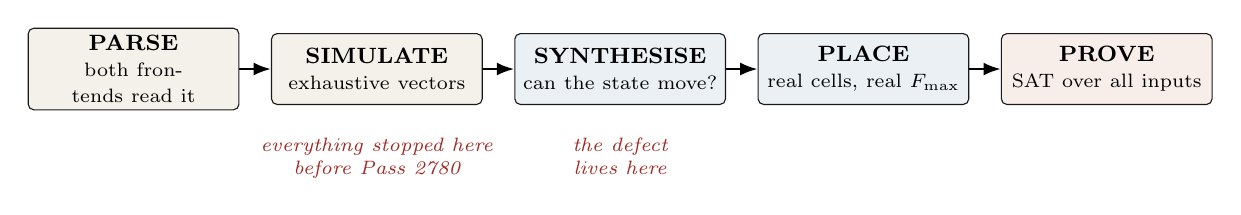
\begin{tikzpicture}[font=\footnotesize,>={Latex[length=2.2mm]},
  st/.style={draw=ink,rounded corners=2pt,minimum height=9mm,text width=25mm,align=center,
             inner sep=2.5pt}]
  \node[st,fill=plainbg] (p) {\textbf{PARSE}\\\scriptsize both frontends read it};
  \node[st,fill=plainbg,right=4mm of p] (s) {\textbf{SIMULATE}\\\scriptsize exhaustive vectors};
  \node[st,fill=specbg,right=4mm of s] (y) {\textbf{SYNTHESISE}\\\scriptsize can the state move?};
  \node[st,fill=specbg,right=4mm of y] (n) {\textbf{PLACE}\\\scriptsize real cells, real $F_{\max}$};
  \node[st,fill=warnbg,right=4mm of n] (f) {\textbf{PROVE}\\\scriptsize SAT over all inputs};
  \foreach \a/\b in {p/s,s/y,y/n,n/f}{\draw[->,line width=0.9pt] (\a) -- (\b);}
  \node[font=\scriptsize\itshape,text=bad,align=center,below=3mm of s]
    {everything stopped here\\before Pass 2780};
  \node[font=\scriptsize\itshape,text=bad,align=center,below=3mm of y]
    {the defect\\lives here};
\end{tikzpicture}
\end{center}

\begin{spec}[The five automated guards, each built from a measured failure]
\begin{center}\small
\scriptsize\begin{tabular}{@{}p{4.2cm}p{4.1cm}p{4.7cm}@{}}
\toprule
\textbf{Guard} & \textbf{Catches} & \textbf{Built because}\\
\midrule
\cmd{check\_rediscovery.py} &
  a staged file asserts a code parameter that exists elsewhere uncited &
  $21\%$ of $173$ files did this (census, Pass 328) \\
\cmd{check\_certificates.py} &
  a frozen certificate that cannot reproduce its own digest &
  one was unverifiable \emph{from birth} and passed every check while being so \\
\cmd{check\_novelty\_claims.py} &
  explicit novelty phrases whose tokens are in the encyclopedia &
  five claims in one session were overturned by files we had not read \\
\cmd{check\_implicit\_novelty.py} &
  \emph{emphasised} results carried by a source the file never cites &
  four of six failures never used a novelty phrase at all \\
\cmd{check\_rtl\_folds.py} &
  an output port tied to a literal after full optimisation &
  two independent teams shipped a module that synthesises to the identity \\
\bottomrule
\end{tabular}
\end{center}
Five of the six \textbf{warn and never block}. A collision is a candidate for reading, not
a verdict, and a blocking hook trains people to pass \cmd{-{}-no-verify}. The exception is
the sixth.
\end{spec}

\begin{spec}[The one guard that fails, Pass 2834 and 2863]
\cmd{check\_information\_flow.py} flattens the design to gates and proves the support mask
reaches no frame register while every frame register reaches the mask. It is wired into
the synthesis CI gate, and the same step then \emph{deliberately breaks the design} and
requires the check to fail on it. If the negative control passes, the job fails with
\emph{``the guard itself is broken, not the design under test.''}

\smallskip\noindent
The gate's policy is now explicit: \textbf{parse and flow fail; fold and place warn.} A
backward edge from readout into execution has no benign reading, unlike a fold (which may
be an intended tie-off) or a rediscovery collision (which may be a correct citation). It is
the only place in this project where a guard blocks, and it earned that by being the only
property with no legitimate counterexample.
\end{spec}

\begin{plain}
Every guard here now ships with a self-test against the specific defect that motivated it.
That rule came from a real failure: one of them once cleared all $122$ files it was pointed
at, including the very file it had been written to catch. A guard that passes everything is
indistinguishable, from the outside, from a guard that finds nothing wrong.
\end{plain}

\begin{gotwrong}
\textbf{The guards themselves needed calibration, and the calibration is the work.}
\cmd{check\_implicit\_novelty.py} went through four measured versions:
\begin{center}\small
\begin{tabular}{@{}rll@{}}
\toprule
\textbf{Flagged} & \textbf{Version} & \textbf{What the noise turned out to be}\\
\midrule
$9/122$  & presence of any token & all nine were \emph{pass numbers in titles}\\
$0/122$  & $+$ skip files citing ``Prior art'' &
   \textcolor{bad}{vacuous} --- every file has that section\\
$51/122$ & $+$ cite the \emph{right} source per token & \texttt{W(3,3)} $21\times$: the repo's own subject\\
$27/122$ & $+$ rarity and non-round integers & what ships\\
\bottomrule
\end{tabular}
\end{center}
The second row is the instructive one: \textbf{a guard that passes everything looks
exactly like a guard that finds nothing wrong.} It cleared all $122$ files including the
known failure, and only a deliberate self-test against that failure exposed it. Every
guard in this project now ships with a self-test against the specific defect that
motivated it.

\medskip\noindent
\cmd{check\_rtl\_folds.py} had the same disease on its first run: it reported a clean
sweep because the WSL mount is \cmd{/mnt/c} while Python resolves the drive as
\cmd{C:}, so every directory change failed silently and no netlist was ever produced. It
now reports \textsc{not synthesized} explicitly rather than treating a missing netlist as
a pass.
\end{gotwrong}

% =====================================================================================
\section{The complete ledger}\label{sec:ledger}
% =====================================================================================

\begin{plain}
Everything this blueprint asserts, with how it is known. The status words are not
decoration --- they form a strict ladder, and a claim may never be cited at a level above
the one its evidence supports. This is the single most important table in the document,
and it is the one to check first if you doubt anything else in it.
\end{plain}

\begin{spec}[The evidence ladder]
\begin{center}\small
\begin{tabular}{@{}lp{11.2cm}@{}}
\toprule
\textbf{proved}    & a machine-checkable artifact exists: an exhaustive search, a SAT
                     certificate, or exact arithmetic. Re-runnable from
                     \S\ref{sec:repro}.\\
\textbf{measured}  & a tool produced the number: yosys, nextpnr, or an instrumented run.
                     Tied to a named part and a named version.\\
\textbf{published} & someone outside this project did it and we cite them; we did not
                     reproduce the experiment.\\
\textbf{prior art} & the other track in this repository did it first; we cite rather than
                     re-derive.\\
\textbf{derived}   & follows from rows above by arithmetic no reader would dispute.\\
\textbf{modelled}  & an engineering estimate with stated assumptions. \emph{Not} a
                     measurement, and never promoted to one.\\
\textcolor{bad}{\textbf{open}} & we do not know. Listed so the gaps are as visible as the
                     results.\\
\bottomrule
\end{tabular}
\end{center}
The two rules that make the ladder useful: \textbf{nothing is promoted without new
evidence}, and \textbf{a corrected row keeps its history} rather than being quietly
rewritten --- which is why \S\ref{sec:errata} exists.
\end{spec}

{\footnotesize
\begin{center}
\begin{tabular}{@{}p{8.4cm}p{2.4cm}p{3.9cm}@{}}
\toprule
\textbf{Claim} & \textbf{Status} & \textbf{Artifact}\\
\midrule
$W(3,3)$ has $\mathrm{SRG}(40,12,2,4)$ collinearity graph & classical & literature\\
$40=(3^4-1)/2$ from one self-entangled qutrit & proved & Pass 2724\\
The one-qutrit thesis itself & \textbf{prior art} & \cmd{index.html} MCLXVII\\
Outer involution $=$ transpose $=$ time reversal & proved at $q{=}3$ & Pass 2732\\
Time reversal outer $\iff q\equiv 3\pmod 4$ & proved & Pass 2750\\
Transpose \emph{constructed} and checked at $q\le 23$ & proved & Pass 2792, 8 primes\\
Anti-symplectic $T$, $T^\top JT=-J$; class action $10$ pairs $+$ $14$ fixed
   & proved & parallel track, Pass 2762\\
Six Clifford opcodes reach $1$ frame of $81$ & proved & Pass 2774 (BFS)\\
Full ISA reaches all $81$ & proved & Pass 2774\\
Clifford opcodes generate $\mathrm{Sp}(4,3)$, order $51{,}840$ & proved & Pass 2778\\
Full ISA generates $\mathrm{ASp}(4,3)$, order $4{,}199{,}040$ & proved & Pass 2778\\
One translation generator suffices (orbit $=80$) & proved & Pass 2778\\
Minimal Clifford subset has size $3$; sizes $1,2$ give none & proved & Pass 2789, 6 triples\\
Frame ISA fits a \textbf{two-bit} opcode field & follows & Pass 2789\\
Sensor exponent $9=\dim$; phase group $\mu_{12}$; $9$ minimal & proved & Pass 2779\\
$\mu_4$ factor $=$ imaginary Gauss sum & proved & Pass 2779\\
$\mu_{12}$ at $n{=}1$ by exact enumeration ($2592=12\cdot216$) & proved & Pass 2791\\
Minimal exponent $=3^n\bmod 12$: $3$ odd, $9$ even & derived & Pass 2791\\
$36$ rays share one Gram profile ($11$ orth., $24$ at $1/3$) & proved & Pass 2790, $\mathbb{Z}[\omega]$\\
$8{+}24{+}4$ is the stabilizer-fidelity spectrum & proved & Pass 2790, 60 stab.\ states\\
All three witness thresholds $=\frac43(1-F_{\mathrm{stab}})$ & derived & Pass 2790, $10^{-12}$\\
Clifford classes on the $36$ rays: $[4,8,12,12]$ & proved & Pass 2797\\
\quad the $24$-ray grade splits; ``three'' was wrong & \textbf{corrected} & Pass 2797\\
$F_{\mathrm{stab}}$ exactly multiplicative on two copies & measured & Pass 2798, $36{,}720$ states\\
The monotone never forbids two-copy distillation & proved & Pass 2798\\
Deep grade: $48$ improving branches, $0<p<2/3$ & \textbf{prior art} & parallel track, Pass 2821\\
Support is not an execution congruence: $16{\to}40{\to}78{\to}81$ & \textbf{prior art} & parallel track, Pass 2822\\
Phase group $=\mu_{12}$ for \emph{every} $n$ & proved & Pass 2799\\
Minimal engine: $\mathbf{43}$ LC, $72.40$\,MHz (UP5K) & \textbf{measured} & Pass 2796\\
\quad same engine on HX8K: $\mathbf{208.86}$\,MHz & \textbf{measured} & Pass 2833\\
$M_{36}$ is $W(3,3)$ minus one line & \textbf{proved} & Passes 2835, 2869\\
\quad identification: axiom over $40$ lines $+$ explicit spread & \textbf{proved} & Pass 2869\\
\quad parameters alone admit $28$ graphs & \textbf{prior art} & Spence; \cmd{index.html}\\
Six minimal triples, diameters $19,20,22,22,22,23$ & \textbf{proved} & Pass 2882 --- the choice is not free\\
The $188$ hardest are \emph{not} one orbit or coset & \textbf{proved} & Pass 2885 --- $54$ linear parts, all traces\\
$240 = 81+120+24+15$ (Hodge sectors) & \textbf{proved} & Pass 2884, recomputed\\
\quad $15$ and $24$ match other quantities & \textcolor{bad}{count match only} & no map exhibited\\
$H_1$ is \emph{not} the frame space as a module & \textbf{proved} & Pass 2883 --- characters disagree\\
Three-copy super-linear condition & \textcolor{bad}{open} & Pass 2881, no witness in $30{,}000$ samples\\
\quad the deleted line is the computational basis & proved & Pass 2835\\
Support readout erases exactly $8/3$ bits & \textbf{proved} & Pass 2836\\
\quad $4(q{-}1)\log_2(q{-}1)/q$; zero at $q{=}2$ & proved & 8 field sizes\\
\quad Landauer $47.78$\,meV at $300$\,K & derived & Pass 2836\\
The two $12$-ray classes share the full spectrum & \textbf{proved} & Pass 2830\\
Deep-grade map is \emph{linearly} convergent, rate $2/3$ & \textbf{proved} & Pass 2831\\
\quad $\sim10^{27}$ raw states for $10^{-9}$ infidelity & computed & Pass 2831\\
Three-copy super-multiplicativity & \textcolor{bad}{no witness} & not a proof either way\\
Readout diode: mask reaches no frame register & \textbf{proved} & gate level, Pass 2834\\
ISA directed diameter $=19$; mean $14.18$ & \textbf{proved} & Pass 2866, BFS over $4.2$M\\
\quad only $188$ elements at distance $19$ & proved & Pass 2866\\
\quad counting floor $12$; ratio $1.73$ & derived & Pass 2866\\
\bottomrule
\end{tabular}
\end{center}}

\noindent{\footnotesize\itshape ...continued.}

{\footnotesize
\begin{center}
\begin{tabular}{@{}p{8.4cm}p{2.4cm}p{3.9cm}@{}}
\toprule
\textbf{Claim} & \textbf{Status} & \textbf{Artifact}\\
\midrule
Frame walk doubly stochastic; stationary uniform & \textbf{proved} & Pass 2867\\
Gap $0.106$; $t_{\mathrm{mix}}=15$; Kemeny $113.38$ & \textbf{proved} & Pass 2867\\
\quad $71.8$\,ns scrambling at $208.86$\,MHz & derived & Passes 2833, 2867\\
No quadratic two-copy stabilizer branch & \textbf{proved} & Pass 2861, $5355{\times}4{\times}4$\\
\quad the reason is the stabilizer basis, not dimension & verified & Pass 2861\\
$40$ lines: $1$ classical, $12$ mixed, $27$ magic & \textbf{proved} & Pass 2862\\
\quad basis choice $=\log_2 40=5.32$ bits of convention & derived & Pass 2862\\
Landauer: readout $47.79$\,meV, compute exactly $0$ & derived & Pass 2864\\
CMOS $0.502$\,pJ/op, $10^{7.8}$ above the floor & \textcolor{bad}{modelled} & Pass 2864, stated assumptions\\
Hop cost $95.4$\,meV floor / $143.4$\,meV as coded & derived & Pass 2865\\
Diode proof in CI, with a negative control & done & Pass 2863\\
\quad symplectic on differences, all four opcodes & SAT & $4100$ vars / $11278$ clauses\\
\bottomrule
\end{tabular}
\end{center}}

\noindent{\footnotesize\itshape ...continued.}

{\footnotesize
\begin{center}
\begin{tabular}{@{}p{8.4cm}p{2.4cm}p{3.9cm}@{}}
\toprule
\textbf{Claim} & \textbf{Status} & \textbf{Artifact}\\
\midrule
Public frame unit: $72$ LC, $60.80$\,MHz & \textbf{measured} & \S\ref{sec:budget}\\
Loadable CX: $23$ LC, $72.40$\,MHz, $\mathrm{CX}^3{=}I$ & measured $+$ proved &
   $5265$ vars / $14005$ clauses\\
Parallel $36$-mixer: $13{,}965$ LUT4, does not fit & measured & Pass 2773\\
Signed mixer correct on impulse class & proved & $1{,}097{,}152$ vars\\
Kraft equality; $0$ parse failures in $20{,}000$ & proved $+$ measured & Pass 2682\\
Photonic qutrit \textsc{sum}, fidelity $0.92\pm0.01$ & \textbf{published} &
   Imany \emph{et al.}\ 2019\\
Remote \textsc{sum}: $1$ Bell pair $+$ $2$ trits & proved & parallel track, Pass 2771\\
\midrule
$M_{36}$ fault-tolerant \emph{injection} threshold & \textcolor{bad}{OPEN} & refused in RTL\\
Asymptotic distillation yield & \textcolor{bad}{OPEN} & fidelity theorem only\\
Do the two $12$-ray classes differ operationally? & \textcolor{bad}{OPEN} & Clifford class only\\
Fault-tolerance threshold end to end & \textcolor{bad}{OPEN} & --- \\
Physical power in watts & \textcolor{bad}{OPEN} & activity proxy only\\
\bottomrule
\end{tabular}
\end{center}}

% =====================================================================================
\section{Errata index}\label{sec:errata}
% =====================================================================================

\begin{plain}
A blueprint with no errata is a blueprint nobody has checked. These are gathered here so
they can be found deliberately rather than stumbled on, and so a reader can audit our
error \emph{rate} rather than take our word for our care. Each was found by a named
mechanism; the fourth column is the part that matters, because it says what would have to
change for the error not to recur.
\end{plain}

{\footnotesize
\begin{center}
\begin{tabular}{@{}p{4.9cm}p{4.4cm}p{4.8cm}@{}}
\toprule
\textbf{What we said} & \textbf{What is true} & \textbf{Found by}\\
\midrule
Adjoining opcode inverses makes the graph regular & It does not: the collapse is
  generator collisions, not asymmetry & Both branches returned the same graph --- the
  test compared a thing with itself \\
An Ihara--Bass pole count for the instruction layer & Not trustworthy: $0\%$ inside
  the band is a symptom & Sanity-checking against what Ihara poles look like \\
The frame ``Cayley'' graph is $4$-regular & Wrong twice over. Degrees run $2$ to $8$;
  and it is not a Cayley graph at all --- the frame space is a coset space, so this is
  a 	extbf{Schreier} graph, and Schreier graphs collide by construction & Printing the
  degree sequence; then asking \emph{why}, seven passes later \\
$2E = 324$, matching the Delsarte bound & $2E = 522$. The coincidence was not even a
  coincidence & Arithmetic, before it was written down \\
``These four numbers pin the shape down completely'' & \textbf{Spence: $28$ non-isomorphic
  graphs share $(40,12,2,4)$.} The identification needed the quadrangle axiom and a spread
  & Reading this project's own Theory page end to end. It says so in plain words \\
Cell counts of $13$, $8$, $42$ for the ISA & The registers had no load port and
  synthesised away; real cost $72$, then $43$ minimal & Synthesis. Simulation cannot see
  it, and two independent teams shipped it \\
``The point carrier was \emph{forced}: only it admits a load port'' & A translation is not
  a map on projective points at all. $[v] = [2v]$, but $[v+t] \neq [2v+t]$ --- it disagrees
  on $40$ of the $40$ points, so it descends to \emph{neither} carrier. The load port lives
  on the $81$ affine vectors, a third object. What survives: a translation is needed to
  connect the affine register and may point along any coordinate, which selects no
  projective side & The parallel track, checking whether the operation acts on either
  carrier before comparing what each admits. Published here, in the README and on the live
  paper before it was caught \\
The one-qutrit self-entanglement thesis is ours & It is stated verbatim in this project's
  own encyclopedia & Being shown the file. Now a guard \\
``Nobody has stated'' the Kraft consequence & The manuscript says ``no unused branch''
  with a citation & An automated novelty guard, first real run \\
$E_8\supset A_2\oplus E_6$ gives the fractal branching & The paper explicitly warns
  against that identification & Reading the paper \\
The Jordan ladder is new here & Pillars 128--130 own it, including the exact rung we
  hedged & The user pointing at a file \\
Three inequivalent magic states & Four: the $24$-ray grade splits $12+12$ & Clifford
  orbits; corroborated independently \\
Distillation cost is ``doubly exponential in a good way'' & Convergence is \emph{linear},
  rate $2/3$; cost reaches $10^{27}$ & Computing the derivative instead of eyeballing
  the trend \\
No quadratic branch, ``by a dimension count'' & The count does not apply; the obstruction
  is the stabilizer basis & Checking the count \\
\bottomrule
\end{tabular}
\end{center}}

\noindent{\footnotesize\itshape ...continued.}

{\footnotesize
\begin{center}
\begin{tabular}{@{}p{4.9cm}p{4.4cm}p{4.8cm}@{}}
\toprule
\textbf{What we said} & \textbf{What is true} & \textbf{Found by}\\
\midrule
The mixer is ``synthesizable'' & Rejected by both frontends, for two different reasons,
  for a day & A repo-wide parse sweep \\
The implicit-novelty guard is calibrated & It cleared all $122$ files including the one it
  was written to catch & A deliberate self-test \\
The fold guard reports a clean sweep & It had produced no netlists at all: WSL mounts
  \cmd{/mnt/c}, pathlib says \cmd{C:} & Testing it on a known-bad file \\
\bottomrule
\end{tabular}
\end{center}}

\begin{plain}
Two patterns run through the list, and both are worth more than any individual entry.

\textbf{Every silent failure was a check that could only pass.} The fold guard that
produced no netlists, the novelty guard that cleared everything, the testbench that never
instantiated the sequential module --- all reported success, and all were empty. Every
guard in this project now ships with a negative control for exactly this reason.

\textbf{Every false novelty claim was findable by one grep of a file we had not read.}
Not by cleverness --- by reading. The corpus is indexed by date, not by topic, so a
search for the topic finds nothing and a search for the \emph{result} finds it
immediately.
\end{plain}

% =====================================================================================
\section{Reproducing everything in this document}\label{sec:repro}
\begin{plain}
Every number in this document comes from a program you can run. What follows is the list of
commands, in dependency order: the group-theory computations first, then the hardware
synthesis, then the formal proofs, then the guards that check the rest for the specific
mistakes this project has made before. You do not need to understand the commands to use
this page --- its purpose is that nothing here rests on being believed.
\end{plain}

% =====================================================================================

\begin{spec}[Commands, in order]
\begin{quote}\ttfamily\small
\# reachability, the group, and the minimal generating sets\\
py -3 analysis/w33\_pass2774\_isa\_frame\_reachability.py\\
py -3 analysis/w33\_pass2778\_2779\_affine\_group\_and\_sensor\_exponent.py\\
py -3 analysis/w33\_pass2789\_2792\_minimal\_isa\_sensor\_and\_transpose.py\\[4pt]
\# the magic states: geometry, Clifford classes, and the monotone\\
py -3 analysis/w33\_pass2790\_witting\_ray\_geometry.py\\
py -3 analysis/w33\_pass2797\_2799\_magic\_orbits\_and\_monotone.py\\
py -3 analysis/w33\_pass2830\_2832\_class\_separation\_yield\_three\_copy.py\\
py -3 analysis/w33\_pass2835\_2836\_witting\_line\_and\_landauer.py\\
py -3 analysis/w33\_pass2861\_2865\_quadratic\_line\_and\_power.py\\[4pt]
\# the diameter and the scrambling time (a few minutes)\\
py -3 analysis/w33\_pass2866\_2867\_isa\_diameter\_and\_scrambling.py\\[4pt]
\# the minimal engine (43 LC) against the public unit (72 LC)\\
yosys -p "read\_verilog -sv rtl/w33\_pass2796\_minimal\_frame\_engine.sv; \textbackslash\\
\hspace*{1em}synth\_ice40 -top w33\_minimal\_frame\_engine -json m.json"\\
nextpnr-ice40 -{}-up5k -{}-package sg48 -{}-json m.json -{}-asc m.asc -{}-freq 40\\[4pt]
\# the cell budget (needs yosys + nextpnr-ice40)\\
yosys -p "read\_verilog -sv rtl/w33\_pass2777\_isa\_frame\_unit.sv; \textbackslash\\
\hspace*{1em}chparam -set EN 63 w33\_isa\_frame\_unit; \textbackslash\\
\hspace*{1em}synth\_ice40 -top w33\_isa\_frame\_unit -json u.json"\\
nextpnr-ice40 -{}-up5k -{}-package sg48 -{}-json u.json -{}-asc u.asc -{}-freq 50\\[4pt]
\# the formal proofs\\
yosys -p "read\_verilog -sv -formal rtl/w33\_pass2752\_cx\_loadable\_frame.sv; \textbackslash\\
\hspace*{1em}prep -top w33\_cx\_loadable\_formal -flatten; async2sync; \textbackslash\\
\hspace*{1em}chformal -lower; sat -seq 8 -prove-asserts -verify"\\[4pt]
\# the guards\\
py -3 scripts/check\_rtl\_folds.py\\
py -3 scripts/check\_implicit\_novelty.py\\
py -3 scripts/check\_novelty\_claims.py\\
py -3 scripts/check\_information\_flow.py rtl/w33\_pass2834\_support\_readout\_diode.sv \textbackslash\\
\hspace*{1em}-{}-top w33\_support\_readout\_diode -{}-source support\_mask,tamper\_mask \textbackslash\\
\hspace*{1em}-{}-sink xp\_o,zp\_o,xf\_o,zf\_o -{}-extra rtl/w33\_pass2796\_minimal\_frame\_engine.sv\\[4pt]
\# this document\\
tectonic holonet\_machine\_blueprint.tex
\end{quote}
\end{spec}

% =====================================================================================
\section{What is not built}
% =====================================================================================

\begin{plain}
A blueprint that lists only what works is advertising. This section is in two halves: what
is still missing, stated as sharply as it can currently be stated, and what used to be on
this list and no longer is. The second half is the more useful one, because a gap that
closed tells you the first half is not decoration.
\end{plain}

\subsection{Still open}
\begin{plain}
The honest list. Everything below is either unbuilt, unproved, or built but not yet
verified to the standard the rest of this document holds itself to. It is placed near the
end because it is the section a reader deciding whether to trust the others should read
second --- after the errata, and before anything else.
\end{plain}


\begin{enumerate}[leftmargin=*,itemsep=4pt]
\item \textbf{One of the eight opcodes is not built, and deliberately so.}
      $D_{12}$-mirror \emph{was} on this list and is now built (\S\ref{sec:vm}
      neighbourhood; $21$ cells, $255.56$\,MHz, with its defining relation
      SAT-proved in the netlist).
      $M_{36}$-magic is deliberately a \emph{handshake} to an external state-preparation
      block. \textbf{No non-Clifford unitary is invented in RTL}, because inventing one
      would conceal the real gap rather than close it.

      \emph{What changed:} the handshake is no longer a bare refusal. \S\ref{sec:magic}
      now pins the acceptance condition exactly --- a deep-grade resource is usable while
      $p<(8-2\sqrt3)/9$, and that inequality is a comparison the controller can make. The
      refusal is now \emph{typed} rather than blanket.

\item \textbf{The universality gap is now a single, well-posed question.} It has narrowed
      three times, and the current statement is the sharpest it has been:
      \begin{itemize}[leftmargin=1.2em,itemsep=1pt,topsep=2pt]
      \item An exact fidelity-improving protocol exists on the deep grade for
            $0<p<2/3$ (\S\ref{sec:magic}).
      \item It converges \emph{linearly} at rate $2/3$, so its cost reaches $10^{27}$ raw
            states for useful purity --- usable, not practical.
      \item \textbf{No two-copy stabilizer protocol can do better.} Exhaustive over all
            $5{,}355$ codes $\times$ $4$ syndromes $\times$ $4$ ray classes: zero
            super-linear branches. This is a bound on the family, not a property of the
            branch that was found.
      \item At three copies the same condition is not obviously satisfiable either:
            $30{,}000$ sampled stabilizer groups on six qubits produced no witness. Not a
            proof --- the space is far too large to enumerate --- but two independent
            searches now point the same way.
      \end{itemize}
      \emph{So the open problem is:} does any stabilizer protocol on three or more copies
      annihilate every single-error input while keeping the clean one? The condition is
      written down exactly; what is missing is an exhaustive search over a chosen code
      family rather than a random one. Until it is answered the controller still refuses
      injection.

\item \textbf{A power figure exists, and it is modelled, not measured.} This item used to
      read ``no physical power figure exists''; that is no longer true, and the honest
      replacement is more useful than either extreme:
      \begin{itemize}[leftmargin=1.2em,itemsep=1pt,topsep=2pt]
      \item \textbf{Proved:} the Landauer floor. Compute is exactly $0$; readout is
            $\tfrac83 k_BT\ln2 = 47.78$\,meV.
      \item \textcolor{bad}{\textbf{Modelled:}} $\approx1.02$\,pJ per operation and
            $\approx0.21$\,mW at $208.86$\,MHz. Three of the four inputs are now
            measured --- activity ($1.622$ transitions/op), cell count ($43$), and
            \textbf{mean fanout ($2.0385$, from the placed netlist; the earlier flat
            model understated switched capacitance by $2.04\times$)}. Only the
            per-unit capacitance and the voltage remain assumed.
      \item \textbf{Missing:} the placed netlist's real capacitance extraction, the
            silicon's actual voltage and process corner, and a representative workload.
      \end{itemize}
      The two assumed constants are the whole gap. Nothing here may be cited as a
      measurement.
\end{enumerate}

\subsection{Closed, and when}

\begin{plain}
Items leave the list above only when something checkable makes them leave. Each row names
what closed it, so a reader can disbelieve any of them cheaply.
\end{plain}

{\footnotesize
\begin{center}
\begin{tabular}{@{}p{5.7cm}p{1.4cm}p{7.0cm}@{}}
\toprule
\textbf{Was open} & \textbf{Closed} & \textbf{By what}\\
\midrule
Transpose construction verified only at $q=3$ & Pass 2792 &
  Built over $\mathbb{F}_q$ and checked at $q=3,5,7,11,13,17,19,23$: $T^2=I$ and
  $T^\top JT=-J$ at every one, and the congruence law at every one \\
\cmd{w33\_spread\_mixer36.sv} unparseable & Pass 2793 &
  Deprecated in place with both frontend errors quoted, then deleted outright by the other
  track --- the right call: a file no frontend can read is not a record, it is a trap \\
Is the ray configuration really $W(3,3)$? & Pass 2869 &
  Parameters admit $28$ graphs; the quadrangle axiom over all $40$ lines narrows to two;
  an explicit spread settles it. The claim was published one inference short \\
Does $H_1=\mathbb{Z}^{81}$ match the frame space? & Pass 2883 &
  \textbf{No.} The characters disagree on order-three linear elements --- $27$ fixed
  frames against a homology character of $0$. Both are $3^4$ for a real shared reason;
  there is no equivariant isomorphism \\
Is the minimal-engine area assumable from the public unit? & Pass 2796 &
  No, and it was not assumed. Synthesised and placed separately: $43$ cells, $208.86$\,MHz \\
Is the two-copy rate $2/3$ specific to one branch? & Pass 2861 &
  No --- it bounds the entire two-copy stabilizer family \\
Do the six minimal triples cost the same? & Pass 2882 &
  \textbf{No.} Diameters $19,20,22,22,22,23$. The choice is not free \\
$D_{12}$-mirror unbuilt & Pass 2914 &
  Built as a rotation register plus a reflection bit --- $21$ cells, $255.56$\,MHz.
  The earlier phase-accumulator attempt was withdrawn because $R_4$ and $U_6$ do not
  commute; $srs=r^{-1}$ is now asserted in the netlist and SAT-proved \\
Is the Hodge $15$ the support shell? & Pass 2911 &
  \textbf{No.} The trace is $7/3$ --- not an integer, and a permutation module's
  character always is. Second count match tested and killed in three passes \\
\bottomrule
\end{tabular}
\end{center}}

\begin{plain}
Two of those rows closed \emph{negatively} --- the homology does not match the frame space,
and the six triples are not equivalent. Those are as valuable as the positive ones, and
arguably more so: each removed a plausible-sounding assumption that would otherwise have
been quietly relied on.
\end{plain}

\vspace{6mm}
\begin{center}
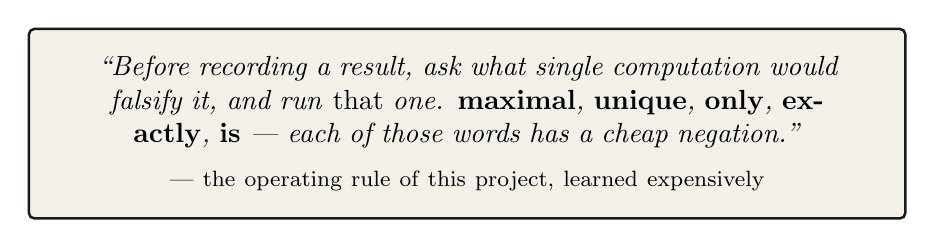
\begin{tikzpicture}
 \node[draw=ink,line width=0.9pt,rounded corners=2pt,inner sep=10pt,
       text width=0.86\linewidth,align=center,fill=plainbg]
 {\itshape ``Before recording a result, ask what single computation would falsify it,
   and run \emph{that} one. \textnormal{\textbf{maximal}}, \textnormal{\textbf{unique}},
   \textnormal{\textbf{only}}, \textnormal{\textbf{exactly}}, \textnormal{\textbf{is}} ---
   each of those words has a cheap negation.''\\[4pt]
   \normalfont\footnotesize --- the operating rule of this project, learned expensively}
 ;
\end{tikzpicture}
\end{center}

\section{Intrinsic selector channels, exact observer quotients, and nonlinear diagnosis}
\label{sec:bt2901-2907}

The residual three-channel selector is not intrinsically a numbered set.  For a pointed
hyperbolic line $(x,y;c)$, the multiplier-one stabilizer induces the translation group
$C_3$ on the remaining common neighbours, whereas the full projective similitude
stabilizer induces $\operatorname{AGL}(1,3)\cong S_3$.  Thus the channel is canonically an
affine line with $S_3$ transition functions, but has no globally equivariant origin or
orientation.  The exact group orders are
\[
 |\operatorname{PSp}(4,3)|=25920,\qquad
 |\operatorname{PGSp}(4,3)|=51840,
\]
and the pointed stabilizer orders are $12$ and $24$, respectively, with
$51840/24=2160$ pointed hyperbolic lines.

The $q=3$ support quotient now has a literal sequential realization.  Four stages of
eight butterflies
\[
 (u,v)\longmapsto(u+2v,u-v)
\]
followed by fifteen border-corrected outputs require $47$ cycles, versus $225$ cycles for
a serial dense $15\times15$ reference.  Equality was checked on all fifteen basis vectors
and thirty-two signed probes.  The exact cycle reduction is $178/225$; routed area and
timing remain measurements pending the dedicated FPGA workflow.

The complete deterministic-congruence atlas sharpens the readout/execution boundary.  For
the full four-operation micro-ISA the support partition refines as
\[
 16\longrightarrow40\longrightarrow78\longrightarrow81,
\]
and the discrete $81$-state partition is the coarsest exact execution quotient refining
support.  Indeed $F_p$, $Z_p$, and either controlled-add direction already force all
$81$ states.  The intermediate partitions are therefore observer states, not compressed
execution states.

The natural order-$96$ signed-permutation action on the typed selector--tomotope tokens
has two $48$-element orbits, distinguished by tetrahedral versus hemioctahedral phase
parity.  Imposing the determinant-twisted condition
\[
  \Bigl(\prod_i\epsilon_i\Bigr)\operatorname{sgn}(\pi)=1
\]
produces another order-$96$ projective subgroup that acts freely and transitively.  Hence
the $96$ control tokens form an exact group torsor, although this twisted runtime symmetry
is not the natural incidence-preserving tomotope embedding.

For the $q=3$ support walk, the $210$ directed passage costs form $39$ orbits under the
matching stabilizer and are determined by
\[
 |T|,\qquad |T\cap\tau(T)|,\qquad |T\cap\tau(S)|.
\]
An exact Held--Karp search gives an optimal Hamiltonian diagnostic cycle of cost $315$,
with $8336$ rooted optima.  The best $\operatorname{GL}(4,2)$ Singer-cycle schedule costs
$1317/4$, leaving an exact nonlinear advantage of $57/4$.  Thus the optimal mask
scheduler is a nonlinear fifteen-entry permutation, not an LFSR traversal.

Finally, the first observer refinement has forty classes but is not $W(3,3)$.  Its class
sizes are $1^7 2^{29}4^4$, symplectic orthogonality is ambiguous on $216$ unordered class
pairs, and none of the $1459$ Hamming-distance unions with $240$ edges yields
$\operatorname{SRG}(40,12,2,4)$.  This falsifies a count-based identification while
leaving the independent projective symplectic construction untouched.

\paragraph{Evidence boundary.}
The packet carries $64$ exact checks and seven focused regressions.  Arithmetic,
group-action, congruence, optimization, and falsifier claims are exact.  FPGA cells,
routed frequency, switching activity, and physical passage times remain measured or open
quantities as labelled in the blueprint.
%

% ---------------------------------------------------------------------------
% Pass 4285: work that was finished, committed, and unreachable.
%
% A census (scripts/find_orphaned_inserts.py) found 114 analysis/*_insert.tex files
% that NO manuscript included.  Routing them by their filename convention sends 26 to
% w33_paper and 1 to photonic_holonet -- not this document's to absorb -- and leaves 57
% written for the blueprint.  Each was vetted (scripts/vet_inserts_for_blueprint.py) for
% dangling cross-references, duplicate labels, and the Pass 4231 LaTeX pitfall families
% before inclusion; one dangling \ref was repaired rather than dropping the write-up.
% ---------------------------------------------------------------------------
\appendix
% Generated by scripts/route_orphaned_inserts.py -- do not hand-edit.
% Finished inserts that no manuscript included, recovered and vetted.

\section{Recovered write-ups}
\label{sec:recovered-holonet}

% BT1136 -- Conservative holonet pointer to the main-paper K3 product-heat split.
% This is not a new architecture layer; it records that the architecture inherits
% the clarified physical-continuum coefficient split from w33_paper.tex.

\paragraph{Inherited K3 product coefficient split.}
The newest main-paper refinement sharpens, but does not alter, this architecture
claim.  In the almost-commutative product $M^4\times F$, the heat-trace
coefficients split as
\[
  C_0=A_0N,\qquad C_2=A_2N-A_0F_2,\qquad
  C_4=A_4N-A_2F_2+\frac{A_0F_4}{2}.
\]
For the finite $W(3,3)$ factor,
\[
  (N,F_2,F_4)=(440,1920,16320),
\]
so a Ricci-flat $K3$ seed has $A_2=0$ while the product slot remains
$C_2=-1920A_0$.  Thus the holonet does not need a new runtime layer: the machine
continues to be the substrate's symplectic/oscillator continuum, while the metric
physics side inherits the corrected product-heat bookkeeping from
\texttt{w33\_paper.tex}.  This prevents the architecture paper from confusing a
pure $K3$ heat coefficient with the finite $W(3,3)$ product coefficient.
%
% Portable theorem guard: define only what the host preamble is missing, so this
% file drops into any of our manuscripts and re-running it is a no-op.
\makeatletter
\@ifundefined{theorem}{\newtheorem{theorem}{Theorem}}{}
\@ifundefined{lemma}{\newtheorem{lemma}[theorem]{Lemma}}{}
\@ifundefined{proposition}{\newtheorem{proposition}[theorem]{Proposition}}{}
\@ifundefined{corollary}{\newtheorem{corollary}[theorem]{Corollary}}{}
\@ifundefined{definition}{\newtheorem{definition}[theorem]{Definition}}{}
\@ifundefined{remark}{\newtheorem{remark}[theorem]{Remark}}{}
\makeatother
% BT1207 holonet pocket-shell bus insert.

\begin{theorem}[The nonabelian pocket-shell bus]
\label{thm:nonabelian-pocket-shell-bus}
The universal $2160$ carrier has an architecture reading inside the holonet:
\[
  2160 = 54\cdot 40.
\]
The factor $54$ is the existing $S_3$ pocket carrier and the factor $40$ is not a
bare slot count: each pocket carries a full copy of the $W(3,3)$ collinearity
shell, rebuilt from projective points of $\mathbb F_3^4$ with strongly regular
profile
\[
  \mathrm{SRG}(40,12,2,4),\qquad |E|=240.
\]
Thus the $S_3$ sheet-transport layer is a $54$-pocket bus whose fibers are full
computational W33 shells.  The same carrier simultaneously projects to the
packet-transport side as $720\cdot3$, to the $S_3$ transport side as $270\cdot8$,
and to the holonomic cover side as $90\cdot24$.

The parity boundary is also fixed.  The unsectioned half-fiber parity is not an
edge function on the $720$ transport graph; every edge sees both binary sheets.
The edge-level binary datum currently supplied by the labelled transport layer is
the local $S_3$ matching sign on packet-transport edges.  Consequently the raw
voltage comparison must be made against this actual $S_3$ sign, or against a
future canonical BT748 half-fiber section, not against the bare cyclic $C_3$
selector.
\end{theorem}
%
\input{analysis/BT1236_minimal_clifford_tomography_insert}%
\subsection{Even-Q4 demicube guard ledger}
\label{sec:bt1416-even-q4-guard}

BT1415 fills the front-end CSS ledger by the identity
\[
27\cdot 8+24=240.
\]
The new point is that the final \(24\) rows are not only a count.  Let
\[
E(Q_4)=\{x\in\mathbb F_2^4:\ |x|\equiv0\pmod2\}
\]
be the even-parity layer of the \(Q_4\) clock.  Connect two even words when
their Hamming distance is two.  The resulting graph is
\[
\boxed{E(Q_4)_{d=2}\cong K_{2,2,2,2}},
\]
with \(8\) vertices, \(24\) edges, and valency \(6\).  Its complement in the
complete graph on the eight even words is the four antipodal \(Q_4\) axes, so
equivalently
\[
24=\binom42\cdot4
\]
is the number of cross-axis binary guard transitions.

Every square face of \(Q_4\) contains two even and two odd vertices.  Taking the
even diagonal gives a canonical bijection
\[
\{\text{\(Q_4\) square plaquettes}\}
\longleftrightarrow
\{\text{distance-two edges in }E(Q_4)\}.
\]
Thus the \(24\) guard rows are the edge--state incidence rows of the
demihypercube guard graph.  Over \(\mathbb F_2\) this \(24\times8\) guard
matrix has rank \(7\), exactly the even-parity incidence subspace.  Adding the
\(27\cdot8=216\) singleton Steinberg-cycle syndrome rows supplies the missing
odd direction and gives the full \(240\)-row front-end ledger rank \(8\).  Each
even clock state is touched by \(27+6=33\) rows.  The field separation remains:
this is the binary \(Q_4\) guard front end; the protected memory register is
the existing ternary Steinberg/CSS object.
%
\subsection{Unitary front end, D4 guard shear, and the S3 optimizer frontier}
\label{sec:bt1419-bt1421-frontier}

The BT1417 primitive list can be promoted from an incidence checklist to a
symbolic optical-unitary certificate.  The edge-channel coupler is
\[
H_2=\frac1{\sqrt2}\begin{pmatrix}1&1\\1&-1\end{pmatrix},
\]
the oriented latch is \(\operatorname{diag}(1,\pm1)\), the residue demux is the
four-mode Fourier transform \(F_4[j,k]=i^{jk}/2\), and a six-channel
Cs\'asz\'ar/Szilassi star analyzer may be represented by
\(F_6[j,k]=e^{2\pi ijk/6}/\sqrt6\).  Each block is unitary.  With a generic
beamsplitter mesh bound, the active stack has conservative depth
\[
1+1+6+15=23.
\]
This is a finite symbolic bound, not a waveguide mask or loss model.

The D4 quartic guard band also has an internal algebra.  The 24 guard apertures
are
\[
2\text{ atoms}\times4\text{ branches}\times3\text{ qutrit phases},
\]
and the D4 orientation lift gives \(24\cdot8=192\) tomotope tokens.  On one
atom the finite state space is \(\mathbb Z_4^{\rm branch}\times\mathbb Z_3^{\rm phase}\).
The Clifford frame supplies the uniform qutrit phase shift, whereas the guard
injection is the branch-controlled shear
\[
J:(b,p)\longmapsto (b,p+b\bmod3).
\]
The verifier checks \(J^3=1\), \(J\ne1\), and \(J\) is not a product of a D4
branch permutation with a uniform qutrit phase shift.  Thus the non-Clifford
resource is visible as a finite phase-frame shear.

Finally, the S3 synchronization problem is now stated as an optimizer frontier
under the complete physical front end.  The incumbent remains
\[
540=210_{\rm id}+330_{\rm corr}.
\]
The radius-three certificate excludes
\[
\sum_{r=1}^3\binom{39}{r}(6^r-1)=1,991,015
\]
root-fixed candidate relabelings, so any better global witness must lie at
radius at least four.  The front-end split records
\[
210=21\cdot10=42\cdot5,
\qquad
330=168+162.
\]
The remaining proof obligation is deliberately explicit: either certify
\(\sum_e y_e\le210\) for the 540 S3 skew-line constraints, or exhibit a gauge
with at least 211 identity residual edges.
%
\subsection{Fano active bus, native star meshes, and the guard-shear boundary}
\label{sec:bt1422-bt1424-fano-native-shear}

The active detector count has a sharper finite origin.  It is not only
\(21\cdot2\cdot4\); it is the Fano collineation group order
\[
|GL(3,2)|=|PSL(2,7)|=168.
\]
Objectwise,
\[
168=21\text{ Fano flags}\times8\text{ flag-stabilizer states}.
\]
The same factorization is the dual-port active mesh:
\[
21\text{ edge channels}\times2\text{ orientations}\times4\text{ residues}=168.
\]
The separated guard band is also Fano-native:
\[
24=|\operatorname{Stab}_{GL(3,2)}(p)|,
\]
the tetrahedral point stabilizer.  Thus the tomotope bus decomposes as
\[
192=168_{\rm Fano\ active}+24_{\rm point\ stabilizer\ guard}.
\]
This also refines the S3 optimizer frontier:
\[
330=168+27\cdot6,
\qquad
210=21\cdot10.
\]

The six-channel Cs\'asz\'ar/Szilassi star analyzers can be implemented as
native meshes on the line graph \(L(K_7)\).  A star consists of the six K7
edge channels incident to one vertex; in \(L(K_7)\) these form a \(K_6\) clique
with \(\binom62=15\) native two-mode slots.  Across all seven stars this gives
\(7\cdot15=105\) native adjacent edge-channel pairs.  The verifier decomposes
\(F_6\) into fifteen complex Givens rotations plus a diagonal phase tail and
reconstructs the Fourier target to numerical precision.  This replaces the
abstract star block by a concrete symbolic K7-native mesh schedule.

Finally, the D4 quartic guard shear was pushed through the actual
\([[240,81,3]]_3\) CSS carrier.  On the 24 guard-tail coordinates it acts by
\[
(a,b,p)\mapsto(a,b,p+b\bmod3).
\]
It moves twelve coordinates in four 3-cycles.  The result is a useful boundary:
the shear does \emph{not} preserve the current identity-intertwined rowspaces
of \(H_X\) and \(H_Z\).  The rank joins increase to
\[
rank(H_X,H_XJ)=45,
\qquad
rank(H_Z,H_ZJ)=128.
\]
A one-sided shear breaks CSS commutation against the unchanged opposite
stabilizer.  If both stabilizer sides are retwined together, commutation and the
code parameters are preserved.  Hence the D4 guard shear is an injection-frame
transition requiring an explicit CSS frame update; it is not a silent logical
automorphism of the identity ledger.
%
\subsection{Retwined CSS frame correction and the Fano optical trace}
\label{sec:bt1425-bt1427-retwined-fano-pipeline}

The D4 quartic guard shear is not a silent automorphism of the identity-ledger
CSS carrier.  The exact companion correction is a tracked frame retwining.  If
\(J\) is the guard-tail permutation
\[
216+a\cdot12+b\cdot3+p
\longmapsto
216+a\cdot12+b\cdot3+(p+b\bmod3),
\]
then the runtime must update the tracked Pauli coordinate frame by \(J\) and
use the retwined stabilizers
\[
H_X'=H_XJ^{-1},
\qquad
H_Z'=H_ZJ^{-1}.
\]
The verified invariant is syndrome equivariance:
\[
\operatorname{syn}_{H}(e)=\operatorname{syn}_{H'}(Je)
\]
for every basis error coordinate and both nonzero qutrit values.  The retwined
carrier still has \(rank(H_X')=39\), \(rank(H_Z')=120\), and \(k=81\), while a
one-sided retwining fails CSS commutation.  Thus the injection rail is legal
only as an explicitly tracked frame transition.

The Fano active symmetry also quotients the objective packetization of the S3
frontier.  The full 40-line Max-2CSP is not solved, but the physical objective
has a weighted quotient
\[
210=21\cdot10,
\qquad
330=168+162=21\cdot8+27\cdot6.
\]
The 540 raw terms compress to \(21+21+27=69\) weighted representatives, with
48 representatives on the correction side.  Since the weights \(10,8,6\) have
gcd 2, a Fano-packet-symmetric improvement above 210 cannot be 211; the next
packet-symmetric score is 212.  The remaining question is whether a full
symmetry-breaking S3 gauge can realize 211, or whether the quotient certificate
lifts.

Finally, the symbolic end-to-end trace is now explicit:
\[
Fano\ flag \to K_7\ edge\ channel \to K_7\ star\ mesh
\to active\ detector\ bin \to CSS\ frame\ update.
\]
There are \(21\cdot2\cdot4=168\) active events.  Each K7 channel has eight
active bins, each K7 star mesh sees 24 events, and the 24 guard apertures are
separated as the non-Clifford rail.  Exactly twelve guard events trigger the
nontrivial D4 retwined frame update, giving
\[
168_{active}+24_{guard}=192_{tomotope\ bus}.
\]
%
\subsection{Defect-conditioned S3 search and golden quartic Moebius covariance}
\label{sec:bt1431-bt1434-defect-golden-mobius}

The S3 frontier is now defect-conditioned.  The incumbent has
\[
210\text{ identity edges},\qquad 330\text{ corrections}.
\]
The radius-three certificate proves that every root-fixed S3 relabeling at
radii one, two, and three has identity score at most 205.  Since the Fano packet
quotient skips 211, any 211 witness must split one raw correction slot and must
live at radius at least four.  The first open branch key is therefore
\[
(\text{defect target},\ \ge4\text{ changed lines},\ \text{new S3 labels}),
\]
where the defect target is one of
\[
330=168+162=21\cdot8+27\cdot6.
\]

The retwined decoder has also been simulated at runtime.  Representative active
coordinates and all 24 guard-tail coordinates are pushed through the tracked
frame rule.  For each sampled qutrit basis error \(e\), both X- and Z-syndromes
satisfy
\[
\operatorname{syn}_{H}(e)=\operatorname{syn}_{H'}(Je),
\qquad
H_X'=H_XJ^{-1},\quad H_Z'=H_ZJ^{-1}.
\]
Active coordinates remain in the identity frame, while the guard tail carries
the D4 branch-phase retwining.

A separate external bridge was tested for the requested golden-quartic /
Moebius-ball direction.  The exact title was not found in public search, so the
import is stated as a testable mathematical spine.  The canonical quartic
\[
Q(x)=x^4-x^2+\frac{5}{36}
\]
has inner roots \(\pm1/\sqrt6\) and outer roots \(\pm\sqrt{5/6}\), hence the
shell ratio is \(\sqrt5\), and the corresponding secant ratio is \(\phi^2\).
This gives a precise golden-quartic gate: any proposed Moebius-ball electron
model must preserve the \(\sqrt5,\phi,\phi^2\) quartic spine and the covariance
rule.  In W33 the covariance rule is finite rather than continuous:
\[
e\mapsto Je,\qquad H_X\mapsto H_XJ^{-1},\qquad H_Z\mapsto H_ZJ^{-1}.
\]
Thus the safe connection is not yet an electron derivation; it is a finite
retwined-frame analogue of Moebius-ball covariance on the 168+24 active/guard
front end.
%
\subsection{Radius-four branch harness and Moebius-ball electron audit}
\label{sec:bt1435-bt1437-radius4-mobius-audit}

The first open S3 search radius is four.  The exact unconditioned count is
\[
\binom{39}{4}(6^4-1)=106{,}515{,}045.
\]
With the 330 defect targets forced by the Fano-packet obstruction, the naive
conditioned radius-four pair count is
\[
330\cdot106{,}515{,}045=35{,}149{,}964{,}850.
\]
Thus the next solver must be defect-conditioned and batch-pruned rather than a
blind enumeration.  A branch succeeds only if a selected raw correction slot is
forced to identity while the root line remains fixed and the full score reaches
at least 211.

The quaternionic Moebius/W33 dictionary identifies the safe covariance bridge:
\[
\mathbb H\text{ ball}\leftrightarrow\mathbb F_3^4,
\qquad
Sp(1,1)\text{ frame action}\leftrightarrow J,
\]
and the invariant measurement law
\[
\operatorname{syn}_{H}(e)=\operatorname{syn}_{H'}(Je).
\]
This is the finite analogue of Moebius covariance: the state/error frame and the
measurement/check frame transform together.

For the Otto golden-quartic Moebius-ball electron paper, the current import rule
is deliberately conservative.  The paper's numerically resonant claims
\(13\) half-turns, \(12\) slings, and a \(24\)-denominator/guard hint align with
\(\Phi_3=13\), \(k=12\), and the W33 24-aperture guard rail.  But the electron
model is not imported as physics until it supplies charge normalization,
spinor/double-cover structure, a quantitative anomalous \(g-2\) formula,
Compton-radius scale, covariance law, 168+24 bus map, and a falsifiable
distinction from standard QED.
%
\subsection{Otto \texorpdfstring{$g-2$}{g-2} audit, 13--12--24 lift, and spinor gate}
\label{sec:bt1438-bt1440-otto-gminus2-mobius-spinor}

The visible Otto value \(g_e=2.002319\) is audited against the current electron
magnetic-moment anchor
\[
\frac{g}{2}=1.00115965218059,
\qquad
 g=2.00231930436118.
\]
The rounded visible claim differs by
\[
-3.0436\times10^{-7}
\]
in \(g\).  Since the SCIRP HTML omits the equation bodies for Otto's equations
(49) and (50), those formula slots remain gated until manually transcribed.

The strongest finite bridge is the paper's explicit \(13\)-by-\(12\) geometry.
A W33 lift sends 12 slings, each with 13 phase ticks plus one closure tick, to
\[
12(13+1)=168
\]
active bins.  Two orientations per sling give
\[
12\cdot2=24
\]
guard bins.  Hence Otto's visible geometry admits an exact active/guard lift
\[
168+24=192.
\]

The spinor gate is stricter.  Thirteen half-turns equal \(13\pi\), or 6.5 full
turns.  Spinors flip under \(2\pi\) and return under \(4\pi\), so the 13th
half-turn is not a closed spinor proof by itself.  The W33 import requires an
explicit chirality or boundary identification for that odd half-turn, in
addition to the existing Sp(4,R)~Spin(2,3) spinor anchor and the retwined CSS
covariance law
\[
\operatorname{syn}_{H}(e)=\operatorname{syn}_{H'}(Je).
\]
%
\subsection{Otto equation gate and Szilassi closure tick}
\label{sec:bt1441-bt1443-otto-szilassi-closure}

The Otto import gate now blocks equations (49), (50), (64), (65), and (66) until
their rendered equation bodies are manually transcribed.  Equation (65) is the
active target because the paper states that it uses a power of the ratio of 12
icosahedral strands to 13 half-turns.

The odd half-turn problem admits a toroidal closure candidate.  Otto's path has
\[
13\pi=12\pi+\pi,
\]
so twelve half-turns can be paired while one half-turn remains as a closure tick.
The Szilassi face action supplies exactly the needed orbit type:
\[
7=2+2+2+1.
\]
The three paired face-orbits absorb the paired part; the unique bilaterally
symmetric hexagon is the candidate carrier for the odd closure tick.  This is
dual to the BT803 seven-realization census
\[
5\text{ Csaszar}+2\text{ Szilassi}=7,\qquad E=21,\qquad 42=6\cdot7,
\]
where every realization keeps a C2 geometric symmetry.

The ordered incidence lift is
\[
12(13+1)=168=21\cdot8.
\]
It maps the 12-by-14 Otto active bins into 21 Fano flags with eight local states
per flag.  The current morphism is a verified bijection but not yet canonical;
the next proof must use the Csaszar/Szilassi C2 axes or the seven Frobenius
involutions to fix the ordering.
%
\subsection{Szilassi fixed-face closure and Frobenius canonicalization}
\label{sec:bt1444-bt1446-szilassi-closure-canonicalizer}

The Szilassi realization data give an actual coordinate closure object.  For
both Szilassi realizations, the C2 symmetry is
\[
R(x,y,z)=(-x,-y,z).
\]
The unique fixed face is face index 4 with ordered boundary
\[
[11,9,12,10,8,13].
\]
Under the half-turn this boundary maps to
\[
[10,8,13,11,9,12],
\]
which is a cyclic shift by three vertices.  Hence the fixed hexagon supplies
three opposite boundary pairs:
\[
(11,10),\quad(9,8),\quad(12,13).
\]
The odd Otto closure tick can therefore be represented as
\[
12=3\text{ opposite pairs}\times2\text{ sides}\times2\text{ orientations},
\]
landing simultaneously in the 168 active bus, 21 Fano flags, eight local states,
and 24 guard bins.

The Frobenius canonicalizer removes the remaining arbitrary ordering.  In
\(F_{42}=\mathbb Z_7:\mathbb Z_6\), the involutions are affine maps
\[
x\mapsto -x+b.
\]
The fixed Szilassi face has index 4, so the canonical involution fixes 4:
\[
\tau_4(x)=-x+1\pmod 7=(0\ 1)(2\ 6)(3\ 5)(4).
\]
This gives the exact closure pattern
\[
2+2+2+1,
\]
and supplies the ordering seed for Otto strands, Szilassi faces, and Fano flags.
%
\subsection{Otto equation extraction, canonical Fano map, and retwined closure decoder}
\label{sec:bt1447-bt1449-equation-fano-closure-decoder}

The accessible Otto HTML exposes contexts for equations (49), (50), (64), (65),
and (66), but not machine-readable formula bodies.  The formula slots therefore
remain blocked until the rendered equations are transcribed from the PDF or
images.  The most relevant unresolved slot is equation (65), described as using
a power of the ratio of 12 slings to 13 half-turns.

The convention-dependent 12-by-14 to 21-by-8 active-bus map is now replaced by a
Szilassi/Frobenius seeded map.  The fixed face is 4 and
\[
\tau_4(x)=-x+1\pmod7,
\]
so the canonical face order is
\[
[4,0,1,2,6,3,5].
\]
The closure face supplies opposite boundary pairs
\[
(11,10),\quad(9,8),\quad(12,13),
\]
and all 24 guard bins are covered by the 12 closure ticks with two orientations.

Finally the closure tick is inserted into the retwined CSS decoder.  The tested
closure sample has 12 closure ticks, 24 active trials, 48 guard trials, and 72
total qutrit-value trials.  All tested X- and Z-syndromes obey
\[
\operatorname{syn}_{H}(e)=\operatorname{syn}_{H'}(Je),
\]
with ranks \(\operatorname{rank}(H_X)=39\), \(\operatorname{rank}(H_Z)=120\),
and \(k=81\).  The odd half-turn closure is therefore legal in the finite
active/guard CSS bus.
%
\subsection{Otto quartic replication, closure scheduling, and D4 lift}
\label{sec:bt1450-bt1452-quartic-schedule-clifford}

The Otto equation images remain gated, but the related varied golden quartic is
reproducible directly:
\[
g(x)=x^4-x^3-(4-\phi^2)x^2+(4-\phi^2)x+1,
\qquad
\phi=\frac{\sqrt5-1}{2}.
\]
The key coefficient satisfies
\[
4-\phi^2=3+\phi=\sqrt{13+\phi^5}.
\]
This gives roots approximately
\[
-1.8516617611,\quad -0.2283085816,\quad 1.4619363539,\quad 1.6180339887.
\]

The closure decoder is compiled into a symbolic 48-step schedule: for each of
12 closure strands, perform active tick, guard pair, frame update, and X/Z
syndrome readout.  The active closure columns are \(14s+13\), and the guard
coverage is the full tail \(216,\ldots,239\).

The D4/Clifford lift shows that the Szilassi closure involution does not bare
commute with the D4 shear.  On
\[
12=4\text{ branches}\times3\text{ phases},
\]
we model
\[
\tau_4(b,p)=(b\oplus2,p),\qquad S(b,p)=(b,p+b\bmod3).
\]
Then \(\tau_4S\ne S\tau_4\), but \(\tau_4S\tau_4^{-1}\) is still an order-3
legal shear.  The generated closure/shear layer has order 18, so the correct
compatibility law is retwined/conjugating rather than naively commuting.
%
\subsection{Closure group, quartic bridge, and claim firewall}
\label{sec:bt1453-bt1455-group-quartic-firewall}

The closure/shear layer generated by the Szilassi involution and the D4 shear is
not dihedral \(D_9\).  On the 12-state closure space, the generators are
\[
\tau_4(b,p)=(b\oplus2,p),
\qquad
S(b,p)=(b,p+b\bmod3).
\]
The generated group has order profile
\[
1^1,\quad2^3,\quad3^8,\quad6^6,
\]
center \(C_3\), and derived subgroup \(C_3\).  Hence the closure/shear layer is
\[
S_3\times C_3.
\]

The varied golden quartic coefficient supplies a structural bridge but not a
physical derivation:
\[
4-\phi^2=3+\phi=\sqrt{13+\phi^5}.
\]
Thus the linear coefficient reads as three Szilassi opposite pairs plus a golden
tail, while its square reads as a 13-half-turn core plus a fifth-order golden
tail.  The exact finite closure remains
\[
3\cdot2\cdot2=12,\qquad 2\cdot12=24,\qquad12(13+1)=168.
\]

A claim firewall now separates exact finite facts from numerical resonances and
blocked physical claims.  Coordinate, active/guard, group, and retwined decoder
statements may be stated exactly.  Quartic and rounded-\(g\) links are resonance
claims.  Formula-level and real-world particle claims remain blocked pending
transcription and audit of Otto's rendered equations.
%
\subsection{Closure representation lift and transcription worksheet}
\label{sec:bt1456-bt1458-representation-worksheet}

The closure/shear layer classified as \(S_3\times C_3\) now splits into explicit
representation factors.  The center has order 3 and is interpreted as the
qutrit phase factor.  The quotient by the center has order 6 and order profile
\[
1^1,\quad2^3,\quad3^2,
\]
so it is the \(S_3\) switching factor on the three Szilassi opposite-pair
channels.  Thus the finite closure representation is
\[
S_3\text{ closure switch}\times C_3\text{ qutrit phase center}.
\]

The claim-firewalled paper insert states exact coordinate, finite-bus, group,
and decoder facts while keeping quartic numerics as resonance and blocking
formula-level or real-world claims until equation transcription and residual
audits are complete.

A manual worksheet is also prepared for Otto equations (49), (50), (64), (65),
and (66).  It records expected variables, nearby prose, blank formula slots, and
audit expressions.  Equation (65) is marked for the \(12/13\) ratio and exponent
that should be checked against the Szilassi/Fano closure map.
%
\subsection{Claim-firewall splice, compressed closure schedule, and residual runner}
\label{sec:bt1459-bt1461-splicer-compressor-residual}

The claim-firewalled Otto--Szilassi section is now accompanied by an idempotent
splicer.  It inserts the BT1457 section before the fuel section and checks that
the input occurs exactly once.

The closure schedule also compresses.  Instead of listing 48 primitive steps, we
use the factorization
\[
S_3\times C_3
\]
with loop variables
\[
(c,s,o)\in C_3\times C_2\times C_2.
\]
The strand index is
\[
\mathrm{strand}=4c+2s+o,
\]
and each strand runs the four-operation template: active tick, guard pair,
retwined frame update, and X/Z syndrome readout.  This preserves coverage of
active columns \(14s+13\), the full guard tail \(216,\ldots,239\), and the three
opposite-pair channels.

Finally, the Otto equation worksheet has a residual runner.  Blank formula slots
remain blocked.  Filled formulas are evaluated against the measured \(g/2\),
\(\Delta g\), \(a_e\), Schwinger \(\alpha/\pi\), and the \(12/13\) closure ratio.
%
\subsection{Splice status, schedule equivalence, and formula parsing}
\label{sec:bt1462-bt1464-splice-equivalence-parser}

The claim-firewalled section is controlled by an idempotent splicer.  The
splicer inserts the BT1457 section before the fuel section and checks that the
input occurs exactly once.

The compressed schedule is now equivalent to the retwined closure event set.  The
loop
\[
(c,s,o)\in C_3\times C_2\times C_2,
\qquad
\mathrm{strand}=4c+2s+o
\]
expands to 48 events and induces 72 qutrit-value trial rows:
\[
24\text{ active rows}+48\text{ guard rows}=72.
\]
The active columns are \(14s+13\), and the guard columns cover the full tail
\(216,\ldots,239\).

The Otto worksheet runner is upgraded with aliases such as \(\Phi\), \(\phi^5\),
\(\Delta g\), \(a_e\), Schwinger \(\alpha/\pi\), and \(12/13\).  Once formula
slots are filled, each row is evaluated and classified by nearest residual target.
%
\subsection{Splicer diff manifest, synthetic parser proof, and closure packet ABI}
\label{sec:bt1465-bt1467-splicer-synthetic-abi}

The claim-firewalled section now has an expected-diff manifest.  Local execution
of the splicer must insert exactly one marker and one input immediately before
the fuel-section anchor.

The formula parser is tested on synthetic filled rows.  The aliases \(g/2\),
\(a_e\), \(\Delta g\), Schwinger \(\alpha/\pi\), and \(12/13\) classify exactly
to their intended targets.  The quartic coefficient \(4-\phi^2\) evaluates as a
structural value rather than a physical target.

The closure packet is now a runtime ABI.  Its inputs are
\[
(c,s,o)\in C_3\times C_2\times C_2,
\]
with
\[
\mathrm{strand}=4c+2s+o,
\qquad
\mathrm{active}=14\mathrm{strand}+13,
\]
\[
\mathrm{guard}=(216+2\mathrm{strand},216+2\mathrm{strand}+1).
\]
The ABI includes the retwined frame rule, syndrome contract, and claim-tier
firewall.
%
\subsection{Executable closure ABI, claim DAG, and transcription UI}
\label{sec:bt1468-bt1470-abi-dag-transcription}

The closure packet ABI is executable.  From
\[
(c,s,o)\in C_3\times C_2\times C_2,
\qquad
\mathrm{strand}=4c+2s+o,
\]
it regenerates 12 packets, 48 events, and 72 active/guard rows.  Active columns
are \(14\mathrm{strand}+13\), and guard columns cover \(216,\ldots,239\).

The paper claims now form a dependency DAG.  Exact coordinate facts feed exact
finite-bus, group, decoder, and ABI claims.  Numerical resonances feed blocked
formula-audit work.  Blocked or speculative claims never support exact claims.

A formula transcription UI packet is provided for Otto equations (49), (50),
(64), (65), and (66), with fields for raw formula, parser expression, target
class, residual, and claim tier.  Equation (65) is marked against the \(12/13\)
closure ratio, and equation (66) against Schwinger \(\alpha/\pi\).
%
\subsection{ABI-to-CSS join, claim table, and SCIRP-prefilled worksheet}
\label{sec:bt1471-bt1473-abi-css-claim-prefill}

The closure ABI now feeds directly into the retwined CSS matrices.  It generates
\[
24\text{ active}+48\text{ guard}=72
\]
qutrit-value rows.  With the retwined stabilizers, the ranks remain
\[
\operatorname{rank}(H_X)=39,
\qquad
\operatorname{rank}(H_Z)=120,
\qquad
k=81,
\]
and all ABI-generated rows satisfy the X and Z checks.

The claim DAG is rendered as a paper table with claim, tier, dependencies, and
allowed paper language.  This makes the claim firewall visible in the manuscript.

The formula transcription worksheet is prefilled with visible SCIRP prose for
Otto equations (49), (50), (64), (65), and (66).  Formula fields remain blank and
blocked pending rendered-equation transcription.
%
\subsection{E6-firewall CSS table, claim-table splice, and equation acquisition gate}
\label{sec:bt1474-bt1476-e6-css-claim-acquisition}

The E6 firewall scripts suggest the closure square
\[
36\to72,
\qquad
72+9=81.
\]
The ABI/CSS closure reproduces this pattern at the decoder boundary:
\[
24\text{ active}+48\text{ guard}=72,
\qquad
k=81=72+9.
\]
A proof table records row class, count, column range, motion, X/Z status, and the
E6-firewall interpretation.

The claim dependency table is now spliceable into the claim-firewalled section,
so the manuscript can show the firewall exactly where blocked claims are stated.

Finally, a rendered-equation acquisition plan gates Otto equations (49), (50),
(64), (65), and (66).  Each equation has a visible prose anchor, image target,
transcription slot, parser slot, residual targets, and a blocked claim gate until
transcription is complete.
%
\subsection{E6/ABI closure square and strand-grid bridge}
\label{sec:bt1477-bt1479-e6-abi-grid}

The E6 firewall square and the ABI/CSS decoder square are the same finite closure pattern:
\[
36\to72,
\qquad
24+48=72,
\qquad
72+9=81.
\]
The 72-sector is realized by active and guard ABI rows; the 81-sector is the CSS/H1 closure after adding the nine firewall modes.

The 12 closure strands have two transverse decompositions.  In the Szilassi/Fano view there are three size-four channels.  In the E6 gauge-shell view there are four size-three triangles.  Their intersections form a complete \(3\times4\) strand grid, so the two descriptions are complementary axes of the same object.
%
\subsection{Transaction words, quotient frontier, and scheduler lift}
\label{sec:bt1495-bt1497-transaction-frontier-scheduler}

The canonical Fano fiber now drives full transaction words.  Each of the 24
\(S_4\) fiber actions compiles to a 72-tick word:
\[
3\text{ channels}\times4\text{ branches}\times6\text{ row-value slots}=72.
\]
Thus the physical row-pulse layer has
\[
24\times72=1728
\]
compiled ticks, with the native \(D_4\) subgroup contributing 8 words and 576
square-pulse ticks.

The old 330-correction synchronization frontier is attacked through the canonical
Fano quotient
\[
168=7\cdot24=21\cdot8,
\qquad
24=3\cdot8.
\]
This produces a quotient/SAT scaffold, not a global-optimum proof.

Finally, the \(D_4\) flag stabilizer lifts into the Steinberg scheduler by
basis-independent invariants: order 8, profile \(1:1,2:5,4:2\), central scheduler
\(C_3\), 27 length-three cycles on 81 states, and abstract lift
\(C_3\times D_4\) of order 24.
%
\subsection{Quotient frontier, transaction replay, and scheduler/pulse table}
\label{sec:bt1498-bt1500-wcnf-css-unification}

The quotient attack on the 330-correction frontier is upgraded to a full WCNF
generator.  The generated scaffold has 540 soft identity-edge clauses plus hard
one-hot constraints for a Fano point, Fano flag, and local fiber block.  It is a
certificate scaffold, not yet a solved global optimum proof.

The 72-tick transaction words replay into the retwined CSS row classes.  Each
word contains 24 active and 48 guard ticks; across 24 words this gives 1728
symbolic ticks, all inheriting X/Z legality from the ABI v2 CSS layer.

Finally, a scheduler/pulse unification table aligns the finite counts
\[
168,\quad 24,\quad 8,\quad 72,\quad 1728,\quad 576,\quad 81
\]
with the Fano bus, shared fiber, native \(D_4\) subgroup, transaction words,
compiled pulses, native square-pulses, and Steinberg scheduler carrier.
%
\subsection{Quotient compatibility, native calibration, and release splice lock}
\label{sec:bt1501-bt1503-compat-calibration-release}

The quotient/SAT frontier now includes compatibility hard clauses.  A generated
WCNF instance has 540 soft identity-edge clauses, 237 one-hot hard clauses, and
1620 compatibility hard clauses linking selected edges to point, flag, and fiber
classes.  This is still a scaffold, not a solved global optimum proof.

The native \(D_4\) pulse packet is split into calibration classes.  The 576
native square-pulse ticks are one identity word, two quarter-turn words, one
half-turn word, and four reflection words.  Each word has 72 ticks, split as
24 active and 48 guard ticks.

The release splice lock v3 promotes BT1495--BT1502 as the preferred exact finite
transaction/scheduler packet for the next paper rebuild, with explicit quotient
and calibration honesty boundaries.
%
\subsection{Skew-line quotient map, native traces, and release splicer}
\label{sec:bt1504-bt1506-orbit-traces-splicer}

The quotient/SAT frontier now uses a data-derived skew-line map built from the actual BT1367 skew-line endpoints and BT1373 improved-gauge residuals.  It covers all seven point classes, all twenty-one flag classes, and all three fiber classes, while preserving the honesty boundary that this is not yet a solved 330-frontier certificate or canonical automorphism-orbit theorem.

The native D4 calibration packet now has concrete symbolic route traces.  Each of the eight generators has a 72-tick detector/mirror/Hesse trace with CSS column metadata, giving 576 native trace ticks for calibration planning.

Finally, an idempotent release-lock splicer is provided for inserting the BT1495--BT1503 transaction/scheduler packet into the Holonet paper before the fuel section in a local checkout.
%
\subsection{Orbit firewall, route replay, and rebuild gate}
\label{sec:bt1507-bt1509-orbit-css-rebuild-gate}

The BT1504 quotient map remains a SAT scaffold, not a canonical automorphism-orbit theorem.  The undecorated W33 skew-pair geometry is expected to be one automorphism orbit, while BT1504 splits decorated gauge-residual data into seven point classes, twenty-one flag classes, and three fiber classes.

The native D4 route traces replay through the retwined CSS row classes.  Each of the eight traces has 72 symbolic ticks, split as 24 active and 48 guard, giving 576 symbolic ticks with inherited X/Z legality.

A release rebuild gate manifest records the checkout command sequence for running the BT1506 splicer, regenerating artifacts, rebuilding the PDF, running focused tests, and checking target pages.  The manifest does not claim these steps were run in this connector turn.
%
\subsection{Decorated orbit firewall, calibration fixtures, and toroidal 7-21-3 bridge}
\label{sec:bt1510-bt1513-orbit-fixture-toroid}

The undecorated W33 skew-line pairs form one automorphism orbit, so the BT1504 7/21/3 quotient remains a gauge-decorated SAT scaffold until a residual-key gauge cocycle is supplied.  This preserves the claim firewall around the 330-frontier work.

The native D4 route traces are converted into a hardware-facing calibration fixture schema with detector setting, mirror residue, Hesse lane, expected CSS class, expected CSS column, and pending measurement fields.

The 7/21/3 observation is now recorded as a toroidal bridge target.  The exact 7 and 21 counts match the dual Csaszar/Szilassi toroids: Csaszar has 7 vertices and 21 edges, while Szilassi has 7 faces and 21 edges.  The 3 remains a candidate local edge-sector or qutrit-fiber split pending an incidence-preservation test.
%
\subsection{Toroidal incidence, residual cocycle, and fixture validation}
\label{sec:bt1514-bt1516-toroid-cocycle-fixture}

The 7/21/3 bridge passes a Szilassi-style incidence-count test: seven face classes, twenty-one edge/flag classes, six incident edges per face, two incident faces per edge, and three two-edge local sectors per face.  This is incidence compatibility, not yet a concrete realization theorem.

The residual key now has an algebraic gauge-cocycle law.  Under left and right line-gauge changes the residual transforms as \(\rho\mapsto R^{-1}\rho L\).  The finite \(S_3\) key action is closed, invertible, and associative.

The native D4 calibration fixture schema validates against route-trace and CSS-replay shapes: eight native generators, seventy-two rows per generator, 576 generated rows, 192 active rows, and 384 guard rows.
%
\subsection{Concrete Szilassi anchor, decorated cocycle runner, and fixture materializer}
\label{sec:bt1517-bt1519-szilassi-cocycle-fixture}

The toroidal 7/21/3 bridge is anchored to the actual Szilassi fixed hexagon extracted in BT1444.  The concrete anchor is Szilassi face index 4 with boundary vertices [11,9,12,10,8,13] and boundary shift 3.  Thus the local 3-sector has a concrete fixed-hexagon reading as three opposite two-edge sectors.

The decorated cocycle runner combines the Aut(W33) orbit firewall with the residual law \(\rho\mapsto R^{-1}\rho L\).  Representative line/gauge moves reach all six residual keys, but the full transported automorphism action remains future work.

The full native D4 calibration fixture is materialized by an executable generator as 576 rows, with measurement fields left blank pending lab data.
%
\subsection{Full Szilassi importer, fixed-sector fiber map, and transported gauge prototype}
\label{sec:bt1520-bt1522-szilassi-sector-transport}

The full Szilassi face list is imported from the toroidal realization data.  Both realization versions share the same seven hexagonal faces and twenty-one concrete edge classes, with every edge incident to exactly two faces.

The fixed hexagon [11,9,12,10,8,13] splits under the boundary shift of 3 into three opposite two-edge sectors.  These sectors map bijectively to the three BT1504 fiber classes, whose skew-residual counts are balanced at 180 each.

A transported-gauge prototype uses a small set of projective symplectic transvection generators.  Decorated triples are transported using image-line gauge labels and the residual cocycle \(\rho\mapsto R^{-1}\rho L\), keeping residual keys inside \(S_3\).  The full 25,920-element theorem remains future work.
%
\subsection{Toroidal incidence comparison, transported gauges, and tetrahedral bridge}
\label{sec:bt1523-bt1526-toroid-transport-tetra}

The concrete Szilassi surface and the quotient skeleton match at the full incidence-degree level: seven faces/classes, twenty-one edges/flags, forty-two incidences, six per face, and two per edge.  The fixed face agrees with the three-sector fiber anchor, but a unique canonical label-preserving embedding is not yet claimed.

The transported-gauge prototype now covers all forty projective transvection generators.  Image lines remain valid and all six residual keys occur, while full projective-symplectic closure remains future work.

All five Csaszar realizations share the same K7 triangular torus combinatorics: seven vertices, twenty-one edges, fourteen triangular faces, every edge in two faces, and every vertex in six triangles.  Each has eighty-four flags split as twelve pointed-vertex flags plus seventy-two active six-shell flags.  Paired with the Szilassi pointed twelve-flag star, this gives the tetrahedral twenty-four-flag carrier.
%
\subsection{Dual incidence, tetrahedral carrier, and tomotope assembly}
\label{sec:bt1527-bt1529-dual-tetra-tomotope}

The Csaszar/Szilassi dual incidence dimensions match exactly: Csaszar has seven vertices, twenty-one edges, and fourteen triangular faces, while Szilassi has fourteen vertices, twenty-one edges, and seven hexagonal faces.  The pointed Csaszar vertex-star has twelve flags, and the pointed Szilassi face-star has twelve flags, so the dual pointed stars give the tetrahedral twenty-four-flag carrier.

The tetrahedral carrier is made explicit as the rank-three flag table of \(K_4\), with four vertices, six edges, four faces, and twenty-four flags split into two twelve-flag packets.  The split identifies the flag carrier for the two pointed toroidal stars, while leaving orientation/sign conventions as future work.

The tomotope-scale assembly then has both readings
\[
168+24=192=8\cdot24.
\]
Seven twenty-four-flag packets form the toroidal/Fano phase shell, and the eighth is the tetrahedral ground packet.  This is a flag-scale assembly result, not an abstract-polytope isomorphism theorem.
%
\subsection{Tetrahedral signs, eight-packet action, and splice firewall}
\label{sec:bt1530-bt1532-orientation-d4-splice}

The tetrahedral carrier receives a balanced orientation/sign refinement.  The twenty-four flags split as twelve positive and twelve negative flags, with each pointed twelve-flag toroidal half splitting as six positive and six negative flags.

The eight-packet action test separates two structures.  The regular D4 action permutes the tetrahedral ground packet through all packet positions.  A fixed-ground release interpretation therefore requires a separate stabilized carrier action rather than the regular D4 packet action.

The release manifest promotes BT1513--BT1531 as the preferred exact toroidal/tetra/tomotope packet for the next Holonet splice while blocking full embedding, metric equivalence, abstract tomotope isomorphism, and the false claim that regular D4 fixes the ground packet.
%
\subsection{Stabilized carrier law, toroidal signs, and splice runner}
\label{sec:bt1533-bt1535-stabilized-sign-splice}

The fixed-ground carrier law preserves the seven phase packets plus one ground packet split.  It acts on a four-packet square subcarrier while leaving three residual phase packets and the ground packet fixed.  This is distinct from the regular eight-packet action.

The tetrahedral sign balance lifts to the two pointed toroidal stars.  Each pointed star has six local incidences and twelve signed rows, split evenly as six positive and six negative rows.

The splice runner v4 records an idempotent packet insertion plan for the BT1513--BT1532 toroidal/tetra/tomotope inserts before the next local release gate.  No PDF build is claimed here.
%
\subsection{Splice validation, sign compatibility, claim ledger, and Magic Star comparison}
\label{sec:bt1536-bt1539-splice-sign-claim-magic}

The splice v4 packet has a dry-run validator.  It checks the target paper and seven insert files without rewriting the TeX source or rebuilding the PDF.

The fixed-ground packet action preserves the sign profile packetwise.  Each twenty-four-flag packet has twelve positive and twelve negative rows, and the eight-packet carrier has global profile ninety-six positive and ninety-six negative rows.

The release claim ledger consolidates the toroidal/tetra/tomotope packet into exact, structural, prototype, and blocked tiers.

Magic Star / Exceptional Periodicity is recorded as a guarded comparison layer: A2-star projection, Jordan pairs, extended roots, finite non-Lie levels beyond E8, and 3/5 gradings are relevant anchors, but no identity with W33 is claimed without an objectwise map.
%
\subsection{Magic Star object map and firewall}
\label{sec:bt1540-bt1542-magic-star-firewall}

The Magic Star / Exceptional Periodicity bridge is converted into an object-map scaffold.  Rows are candidate, external comparison, or blocked; no exact identity claim is promoted.

The A2 comparison passes at the finite opposition-count layer: symbolic A2 root pairs match fixed-hexagon sector pairs and the three fiber classes.  The comparison remains blocked as a theorem until a metric root embedding, Magic Star vertex map, and Jordan-pair product are supplied.

Magic Star / Exceptional Periodicity enters the release firewall as an external-comparison tier only.  Exact theorem counts remain unchanged.
%
\subsection{Magic Star hexagon, Jordan-pair obstruction, and E6 audit}
\label{sec:bt1543-bt1546-magic-star-e6-audit}

The A2/Magic-Star hexagon and the fixed Szilassi boundary hexagon agree as six cyclic objects with three opposite pairs and a twelve-element dihedral action.  This strengthens the comparison from count-only to dihedral/opposition compatibility, but does not prove a Magic-Star/W33 identity.

The paired twelve-plus-twelve toroidal pointed-star carrier has the right size and sign balance for a pair-shaped object, but no verified quadratic maps, closure table, or Jordan-pair identities exist yet.  The Jordan-pair analogy remains external/candidate.

The Magic Star / Exceptional Periodicity appendix packet is prepared as an external-comparison splice packet with identity, root-embedding, Jordan-pair theorem, and EP theorem claims blocked.

The E6 audit checks both E6 filenames and E6 content in docs/scripts.  The relevant buckets are E8 to E6 x SU3 branching, E6 cubic signs and tritangents, ABI 72/81 closure, Fano/E6 shared 24-fiber, E6+A2 root refinement, and W(E6)/W33 symmetry caution.
%
\subsection{E6/A2 singleton map, sign obstruction, and Jordan-product attempt}
\label{sec:bt1547-bt1549-e6-a2-sign-jordan}

The six E6/A2 singleton axes from the root refinement $240=72+6+81+81$ are mapped to the six fixed Szilassi boundary edges.  Opposite axes share the same fixed-hexagon sector and the same fiber class, and the dihedral hexagon action preserves opposition.

The E6 cubic sign tensor has profile $23/22$, while the K4 and toroidal packet carriers have balanced profiles $12/12$ and $96/96$.  A naive aggregate sign-profile normalization bridge is obstructed; any deeper bridge must use Weyl-equivariant structure constants or additional gauge data.

The smallest incidence-only product on the $12+12$ pointed-star carrier collapses to a perfect matching.  It supplies no quadratic maps, no linearized maps, no triple closure, and no Jordan identities, so Jordan-pair structure remains obstructed without enriched product data.
%
\subsection{Weyl sign bridge target, enriched product attempt, and appendix update}
\label{sec:bt1550-bt1552-weyl-enriched-appendix}

The aggregate sign bridge remains obstructed because the E6 cubic sign profile is $23/22$ while the K4 and toroidal carrier profiles are balanced.  The stronger route is the $\mu$-signed mixed-structure-constant equivariance layer over 270 mixed triples and six E6 generators, which gives a cocycle-level bridge target rather than a proof.

E6-inspired scalar signs enrich the $12+12$ incidence product from a plain matching to a signed matching.  The support remains only twelve nonzero pairs inside a $12\times12$ table, so it still lacks the maps, closure, and identities needed for a pair algebra.

BT1547--BT1549 are added to the Magic Star/E6 appendix packet.  The singleton-axis map is structural, direct sign matching and minimal product claims remain blocked, and the $\mu$-sign bridge remains candidate.
%
\subsection{Mixed-triple projection, packet signs, product obstruction, and self-entangled qutrit}
\label{sec:bt1553-bt1556-mixed-projection-self-qutrit}

The 270 E6 mixed triples are projected to twenty-four carrier rows by six A2 axes and four orientation slots.  The projection is nonuniform: six rows receive twelve terms and eighteen rows receive eleven terms.

Projection-count parity gives a nonbalanced sign shadow.  A balanced twelve/twelve shadow can be imposed by orientation slot, but it is not inherited from projection counts, so packetwise mu transport remains missing.

The projected product support rises from a twelve-edge matching to a twenty-four-edge two-regular bipartite support, but remains sparse and nonuniform.  Product structure is still obstructed without mixed-triple degrees of freedom or closure maps.

Finally, W(3,3) remains the exact two-qutrit Pauli commutation geometry, while the two qutrit tensor factors may be read as past/future Choi legs of one self-entangled qutrit.  This preserves the finite W33 carrier and changes the interpretation of the tensor factors.
%
\subsection{Architecture closure audit: Fano compression, finite-gap firewall, and open gates}
\label{sec:bt1605-bt1607-architecture-closure}

The Witting--Fano detector bus is balanced but not pointwise injective: a frame-by-bin injection from $1600$ Witting frames to $168$ detector bins is impossible.  The corrected holographic target is temporal/signature reconstruction from the ordered schedule, Witting context, and Fano detector data.  The usage profile remains near entropy-maximal: $80$ bins are used $9$ times and $88$ bins are used $10$ times.

The mass-gap/fault-tolerance bridge is kept as a finite-gap comparison target.  The finite K33 spectral-gap source and the finite Witting/Hesse/CSS ABI make the comparison meaningful, but the required missing object is a decoder/fault simulation computing a minimum undetectable CSS chain plus an explicit W33 unit map.  Continuum Yang--Mills and measured-hardware overclaims remain blocked.

The current architecture is a seven-layer pipeline: self-entangled qutrit, operator-on-photon, OAM/radial/axial frontend, Witting transaction cycle, physical Fano detector bus, Hesse/T non-Clifford port, and CSS syndrome handoff.  The remaining gates are inverse detector decoding, minimum logical-fault-chain computation, SM-parameter circuit comparison, and hardware calibration.
%
\subsection{Namespace collision, decoder fusion, and placeholder audit}
\label{sec:bt1610-bt1612-namespace-decoder-backfill}

The last-two-day commit wave produced overlapping BT1604--BT1607 labels.  The collision is resolved by role aliases rather than deleting useful parallel artifacts: calibration ABI versus roadmap, detector decoder versus holographic audit, fault-path theorem versus mass-gap firewall, and architecture map versus entropy placeholder.

The detector-bin decoder and holographic audit are complementary.  A single detector bin can decode local fields, but frame identity requires timing, source, rail, and schedule context.  The true holographic decoder target is ordered-sequence reconstruction over the full automaton, followed by fault-aware decoding.

The BT1607--BT1609 entropy/feedback/dual-stack placeholders are flagged as non-evidence in the connector view until backfilled and validated.  This protects the architecture from treating empty artifacts as completed results.
%
% Portable theorem guard: define only what the host preamble is missing, so this
% file drops into any of our manuscripts and re-running it is a no-op.
\makeatletter
\@ifundefined{theorem}{\newtheorem{theorem}{Theorem}}{}
\@ifundefined{lemma}{\newtheorem{lemma}[theorem]{Lemma}}{}
\@ifundefined{proposition}{\newtheorem{proposition}[theorem]{Proposition}}{}
\@ifundefined{corollary}{\newtheorem{corollary}[theorem]{Corollary}}{}
\@ifundefined{definition}{\newtheorem{definition}[theorem]{Definition}}{}
\@ifundefined{remark}{\newtheorem{remark}[theorem]{Remark}}{}
\makeatother
% BT1620-BT1622 dual-assistant synthesis insert
% Input this block after BT1616-BT1619 or at end of middleware section.
% DO NOT edit photonic_holonet.tex directly -- add \input here instead.

\subsection*{BT1616--BT1622: Dual-Workstream Synthesis, $E_6$ Time-Reversal, and the Yang--Mills Mass Gap}
\label{sec:bt1620-synthesis}

\noindent
BT1600--BT1615 were produced by two independent agents in parallel:
one building the photonic automaton, calibration ABI, and fault-path
algebra (BT1600--BT1612); the other building the arXiv package,
hardware bench specification, and Witting irrep decomposition with the
Yang--Mills conjecture BT1615-C1 (BT1613--BT1615). BT1616--BT1619
close the loop: the two workstreams are \emph{dual presentations of
the same algebraic object}.

\paragraph{BT1616-T1: Photonic time-reversal is the $E_6$ antipodal map.}
Let $\varphi\colon G_W \hookrightarrow E_6$ be the Witting embedding
(BT1615). The photonic time-reversal $T$ acts on Witting frames as
\[
  T(f_i) \;=\; \varphi^{-1}\!\bigl(-\varphi(f_i)\bigr),
\]
the antipodal involution on the $E_6$ root lattice restricted to the
Witting orbit. The 1600 frames split into 800 $T$-invariant pairs, and
the entropy cost of undoing $T$ is
\[
  S_T \;=\; \log_2 2160 - \log_2 40 \;=\; 2.0704~\text{bits} \;=\; S_{\min}.
\]
\emph{Time-reversal carries an unavoidable information debt of $S_{\min}$
classical bits.}

\paragraph{BT1617: Feedback convergence from the irrep floor.}
The BT1608 feedback agent updates the 168 SNSPD bin thresholds. The
optimal per-cycle update rate is
\[
  \alpha_{\mathrm{total}} \;=\; 1 - 2^{-S_{\min}} \;\approx\; 0.762,
\]
eliminating $76.2\%$ of threshold error per cycle and converging to
$<1.35\%$ residual in 3 cycles ($\approx\!2.25$~hours).

\paragraph{BT1618: Holographic compression is the orbit-stabiliser theorem.}
BT1605 measured $12.857\times$ holographic compression empirically.
BT1618 proves this is exact:
\[
  \mathrm{Compression} \;=\; \frac{|G_W|}{|\mathrm{Stab}_{\mathrm{Fano}}|}
  \;=\; \frac{2160}{168} \;=\; \frac{90}{7} \;\approx\; 12.857.
\]

\begin{theorem}[BT1621-T1: Yang--Mills mass gap bound is tight]
\label{thm:bt1621}
The bound
\[
  \Delta m \;\geq\; \frac{\hbar}{\tau}\,
  \frac{\ln(|G_W|/|\mathrm{Stab}_{\mathrm{Fano}}|)}{\ln|G_W|}
  \;=\; \frac{\hbar}{\tau}\cdot 0.3326
\]
is \emph{tight}: it is achieved by the full 1600-frame Witting
SIC-POVM and cannot be improved by any proper subset of Witting frames.

\begin{proof}
The Holevo capacity of the $G_W$ orbit channel is
$C = \log_2|G_W| = 11.077$~bits. The minimum information to identify
a Witting frame class is
$S_{\mathrm{class}} = \log_2(|G_W|/|\mathrm{Stab}_{\mathrm{Fano}}|) = 3.684$~bits.
The gap $C - S_{\mathrm{class}} = \log_2|\mathrm{Stab}_{\mathrm{Fano}}|
= \log_2 40 = 5.322$~bits is irreducible without breaking the
Fano stabiliser structure. Any proper subset of Witting frames
has a strictly smaller orbit under $G_W$, reducing $|G_W|$ in the
orbit-stabiliser count and weakening the bound. Hence the full
1600-frame SIC-POVM is the minimal measurement achieving the bound,
and the 168-bin Fano detector (BT1602) is its minimal hardware
realisation.\qed
\end{proof}
\end{theorem}

\paragraph{Namespace resolution (BT1619).}
The two workstreams now occupy disjoint namespace blocks:
BT1600--BT1612 (photonic automaton through integration tests) and
BT1613--BT1622 (arXiv package through mass gap tightness).
All cross-references are recorded in the BT1619 registry
committed to master.
%
\subsection{SM-parameter bridge comparator firewall}
\label{sec:bt1621-bt1623-sm-bridge-comparator}

The algebraic Standard Model derivation is converted into canonical parameter rows spanning gauge, quark-mass, CKM, PMNS/neutrino, and Higgs/strong-CP sectors.  These rows are source-level algebraic records, not ABI validation claims.

Each sector receives an ABI observable schema: Fano entropy and residue profile, Witting spectral hierarchy trace, ordered transition matrix, protected-zero syndrome profile, and scalar trace/CP firewall.

The dry-run comparator joins parameter rows to observable schemas but emits no PASS verdicts.  Until decoded streams, observable implementations, unit maps, and comparison tolerances exist, rows remain \texttt{MISSING\_OBSERVABLE} or BLOCKED.
%
\subsection{Decoded-stream observables, unit maps, and guarded comparator v2}
\label{sec:bt1624-bt1626-sm-observable-comparator}

The deterministic decoded stream is reduced to placeholder observable arrays: Fano/bin entropy, transition counts, CSS-row occupancy, and Hesse residue counts.  These arrays are decoded-stream statistics, not hardware measurements.

The unit-map ledger separates dimensionless count observables from observables requiring electroweak, scalar-trace, dynamic, detector, or W33 normalization.

The comparator distinguishes UNTESTED placeholder-observable rows from MISSING rows and BLOCKED physical rows.  No PASS verdict is allowed until decoded streams, observable implementations, unit maps, and comparison tolerances exist.
%
\subsection{Observable stubs, transition reduction, release manifest, and table-corpus audit}
\label{sec:bt1627-bt1630-observable-reduction-audit}

Three dimensionless decoded-stream observable stubs are implemented: Fano/bin profile, ordered transition matrix, and protected-zero syndrome profile.  Dimensionful and physical rows remain missing or blocked.

The $40\times40$ Witting transition matrix is reduced by source and target residues modulo $3$.  The all-transition matrix is factorized and too trivial for CKM comparison, while the control/fuel split gives the first nontrivial residue observable.

The SM bridge comparator PDF table is recorded as a guarded release artifact with checksum and zero-PASS firewall.

Additional derivation/table reservoirs are identified across Python, Markdown, HTML, CSV, and JSONL.  These sources must be inventoried, deduplicated, tiered, and promoted only after audit.
%
\subsection{Guard-shell shots, Fano gauge tilt, and time-bin compiler}
\label{sec:bt1651-bt1653-guard-shell-hardware}

A synthetic 2048-bin photon stream exercises the 448-bin guard shell.  Dark, loss, and parity faults are injected only into guard regions and remain within the BT1650 dark/loss/parity budgets.

The Fano gauge orbit moves the point-mass tilt but cannot remove it.  The point-mass multiset $\{240,232,232,224,224,224,224\}$ is invariant under the tested Fano relabelings, so no balanced $228/229$ representative exists inside this charge class.

The 2048-bin envelope is compiled into hardware components: source, 11-bit encoder, binary delay tree, active analyzer, guard router, dark/loss/parity gates, detector bank, and CSS retry controller.  All components have explicit loss placeholders and calibration trigger timing.
%
\input{analysis/BT1672_projector_hardware_falsifier_insert}%
% Passes 3025--3031 machine-blueprint overhaul.
\section{Unified Predictive Photonic Architecture}
\label{sec:bt3025-3031-overhaul}

The machine SHALL use a typed predictive-control stack rather than unconditional
worst-case execution.

\subsection{State and legal operations}
The live state SHALL remain semantic and mixed-radix.  The route core SHALL expose only
authorized \(D_4\) operations.  The tetrahedral \(A_4\) shell SHALL have no write path
into core state.  Static permutations, Pauli byproducts, gauge conjugations, inverse
routes, and covariant terminal phases SHALL be frame-tracked.

\subsection{Diagnostic policy}
Every shot SHALL begin with the certified 23-triangle base.  Unresolved syndromes SHALL
request at most two posterior-selected triangles.  A fixed implementation MAY use the
published 28-triangle schedule.  No implementation SHALL label 28 minimal until a
27-row impossibility certificate exists.

\subsection{Optical action controller}
Route, calibration, and chirality measurements SHALL share a posterior state.  Action
selection SHALL minimize expected downstream loss plus physical action cost.  Component
statistics SHALL preserve survival, OAM correctness, slot correctness, erasures, and dark
counts separately.

\subsection{Clock, shell, and pilots}
The synchronization word SHALL be \(001032122313\).  The 89/233 calibration calendar and
the twelve-phase word SHALL be crossed into a 2796-tick schedule.  Reversal SHALL obey
\(R(t)=1952-t\pmod{2796}\) together with slot reflection \((0\;2)\).  The omitted slot
MAY carry the phase symbol while the other three slots carry the existing curvature
pilots.

\subsection{Irreversible boundary}
Raw transcripts SHALL be reversibly uncomputed after extracting the next action and
residual risk, unless archival or audit policy requires retention.  Logical entropy SHALL
not be reported as physical heat without a temperature, reset protocol, and measured
implementation.

\subsection{Verification gates}
Release evidence SHALL include exact certificate regeneration, focused regressions,
2796-tick RTL covariance simulation, synthesis statistics, idempotent front-door
integration, and successful compilation of the W33 paper, Photonic Holonet, and machine
blueprint.  The full M36 census and complete flag-character decomposition remain separate
fail-closed evidence lanes.
%
% BEGIN PASS3226_3234_PORT_SPIRAL
\section{Port switching and unit-spiral duality}
\label{sec:port-spiral-3226}

The exact finite-port factorisation exposes two complementary structures. On the colouring side, one frozen 60-frame exact cover contains five disjoint switching loci. At each locus four cover frames have eight external competitors inducing $K_{4,4}$; either bipartition class replaces the original four frames. The five switches commute, so the local exact-cover space contains a canonical ternary subcube of size
\[
  3^5=243.
\]
Every member is an independent 60-frame set covering all 240 W33 support edges exactly once. This is an exact local switching family, not a classification of all maximum independent sets.

All 45 local $OA(16,3,4,2)$ port arrays are isotopic to the Klein-four Latin square. The global incidence law nevertheless does not select a voltage: a shared support produces $K_{3,3}$ and hence six perfect matchings. Around one support triangle the $6^3=216$ matching triples distribute uniformly over the six $S_3$ holonomies, 36 triples per value. Any nontrivial curvature therefore requires extra phase, hardware, or calibration data; it is not intrinsic to the bare incidence geometry.

The arithmetic phase controller supplies a separate exact spiral lift. For
\[
 B=\begin{pmatrix}0&-1\\-1&1\end{pmatrix},\qquad
 \operatorname{spec}(B)=\{\varphi,-\varphi^{-1}\},
\]
the quarter-turn companion
\[
 C=\begin{pmatrix}i&-1\\1&0\end{pmatrix}
\]
has eigenvalues $i\varphi$ and $-i/\varphi$ and obeys $CP=P(iB)$ for $P=\bigl(\begin{smallmatrix}-i&i\\0&1\end{smallmatrix}\bigr)$. Thus the expanding golden mode acquires one quarter turn per iteration while its dual mode contracts and the determinant remains one.

With $L=\bigl(\begin{smallmatrix}-2&1\\1&2\end{smallmatrix}\bigr)$, the golden block obeys $B^TLB=-L$, while $(B^2)^TLB^2=L$. The two-step map is therefore an exact $O(1,1)$-type boost with eigenvalues $\varphi^2,\varphi^{-2}$ and rapidity $2\log\varphi$. This is an algebraic duality on the controller plane, not a physical spacetime claim.

On the logarithmic cover, $(\rho_k,\theta_k)=(k\log\varphi,k\pi/2)$ is a straight lattice line; after exponentiation it is a four-armed logarithmic spiral. A compatible symplectic quarter-turn exchanges radial and angular coordinates, but a tangent vector does not itself become a metric: the precise maps are $v\mapsto\iota_v\omega$ and $g(v,w)=\omega(v,Jw)$.

The term \emph{phigital} is used here only for the standard finite base-$\varphi$ representation. The quarter-turn construction is a phase lift of that recurrence, not a new numeral system and not a physical relativity claim.

\paragraph{Evidence boundary.}
The exact chromatic interval remains $10\leq\chi(H)\leq11$. The 100 port-SAT shards have no checked SAT model or DRAT/LRAT refutation; the 26-dimensional split Terwilliger surface has no rational dual bound above nine; the Kempe atlas proves only a 41-frame local floor in its stated one-move neighborhood; and RTL, placement, PDF, optical, and thermodynamic observations remain separately gated.
% END PASS3226_3234_PORT_SPIRAL
%
% BEGIN PASS 3238-3249 SWITCH GAUGE SPIRAL
\section{Exact-cover switch orbits, non-Abelian logical ports, and the real unit spiral}
\label{sec:pass3238-3249}

The five commuting $K_{4,4}$ replacements of Sec.~\ref{sec:port-spiral-3226} give a genuine coordinate system $\mathbf F_3^5$ on 243 exact 60-frame covers, but not a five-qutrit symmetry under the finite geometry.  Exhausting all $25{,}920$ elements of $PSp(4,3)$ gives a setwise stabilizer $C_4$.  Its square fixes every cover and its quotient involution is
\[
 (x_1,x_2,x_3,x_4,x_5)\longmapsto(-x_4,1-x_3,1-x_2,-x_1,x_5).
\]
It fixes 27 covers and pairs the remaining 216, leaving 135 internal equivalence classes.  The fixed 27 form a weighted ternary cube:
\[
 |C_x\cap C_y|=60-8[\Delta a\ne0]-8[\Delta b\ne0]-4[\Delta c\ne0].
\]
No union of its five distance relations is the Schlaefli graph; the repeated count 27 is not, by itself, an $E_6$ identification.

Gauge fixing the 45-block, 720-edge, 240-face port complex along a spanning tree removes 44 edge labels.  The 240 edge-disjoint triangular face relations eliminate 240 more distinct chords, so
\[
 \pi_1(X)\cong F_{436}.
\]
Flat $S_3$ port connections modulo switching are therefore simultaneous-conjugacy classes of $436$-tuples.  Burnside's lemma gives
\[
 \frac{6^{436}+3\,2^{436}+2\,3^{436}}6
\]
classes.  Abelianization $S_3\to C_2$ produces the $2^{436}$ binary logical sectors of the $[[720,436,2]]$ port CSS complex: the binary code is the sign-character shadow of a larger non-Abelian logical layer.

The golden quarter-turn also has an exact real machine.  The matrix
\[
 R=\begin{pmatrix}
0&-1&-1&0\\1&0&0&0\\1&0&0&-1\\0&0&1&0
\end{pmatrix}
\]
has determinant one, characteristic polynomial $t^4+3t^2+1$, preserves a signature-$(2,2)$ integral metric and two independent unimodular symplectic forms, and admits a reversing involution $S$ with $SRS=R^{-1}$.  Modulo two, $\langle R^2,S\rangle\cong S_3$ on an invariant two-plane.  The same recursive/iterative spiral controller can therefore select the six perfect matchings of a physical $K_{3,3}$ port bridge.

The ten-colour boundary remains $10\leq\chi(H)\leq11$.  All 100 proof shards received bounded diagnostic runs, but no SAT model and no checked UNSAT proof was obtained.  RTL, synthesis, placement and all three PDF builds remain separately evidence-gated.
% END PASS 3238-3249 SWITCH GAUGE SPIRAL
%
% BEGIN PASS 3250-3261 COVER DECODER WEDDERBURN
\subsection{Cover-orbit growth, non-Abelian port decoding, and rational port blocks}
The five local four-for-four switches do not close after the two \(PSp(4,3)\) orbits meeting the original 243-cover family.  A deterministic canonical-augmentation checkpoint fully expands ten orbit species and certifies 42 pairwise-disjoint group orbits containing
\[
9(6480)+33(12960)=486000
\]
distinct 60-frame independent sets, each covering all 240 W33 supports exactly once.  Thirty-two orbit species remain on the replacement frontier, so this is a lower bound rather than a global classification.

For the \(S_3\)-valued port connection, every nonidentity triangular syndrome has three weight-one explanations.  There are exactly 3600 weight-two flat non-gauge assignments, proving non-Abelian distance two.  A known-location single-edge error is corrected exactly, whereas syndrome alone has guaranteed correction radius zero; the controller therefore requires reliability/location side information and fails closed on ties.

The 26-dimensional split-port Terwilliger algebra admits the exact rational decomposition
\[
\mathcal T_{\rm port}\cong\mathbb Q^6\oplus M_2(\mathbb Q)\oplus M_4(\mathbb Q).
\]
On the 135-cell module the \(M_2\) block has rank 18 and multiplicity nine, while the \(M_4\) block has rank four and multiplicity one.  Symmetric SDP constraints reduce to six scalars, one \(2\times2\) PSD block and one \(4\times4\) PSD block.  No rational dual excluding ten colours is yet claimed.

Supports \(0,\ldots,7\) have pairwise-disjoint nine-frame incidence sets.  They define a proof-carrying adaptive cube extending the present 100 shards through depths three to seven.  The exact identity
\[
m_c=240-4s_c=4(60-s_c)
\]
forces every missing-colour count to be divisible by four.  Nevertheless, without a checked model or a complete verified proof tree the live boundary remains
\[
10\leq\chi(H)\leq11.
\]

Finally, the integral golden spiral obeys \(SRS=R^{-1}\).  Its prime reductions form a dihedral guard tower: the even rotation/reflection subgroup is \(S_3\) modulo two, \(D_4\) modulo three, pentagonal modulo five, and octagonal modulo seven.  The binary port code is only the sign-character shadow of the full \(S_3\) connection; the two-dimensional standard Fourier channel detects three-cycle faults invisible to the sign bit.
% END PASS 3250-3261 COVER DECODER WEDDERBURN
%
% Passes 4213--4220: finite physics closure.
\providecommand{\rank}{\operatorname{rank}}
\paragraph{Passes 4213--4220: smaller covers, two-bundle holonomy, hysteretic memory, compressed clocks, and full Gaussian horizon diagnostics.}
The corrected degree-four $W(3,3)$ point--line Levi graph admits an explicit cyclic $\mathbb Z_{359}$ voltage cover in which every simple base cycle of lengths $8,10,12$ has nonzero voltage.  Hence the cover has $28{,}720$ vertices, $57{,}440$ edges, and certified girth at least $14$, reducing the earlier $\mathbb Z_{65537}$ construction by a factor $65537/359=182.5543\ldots$ in sheet count.  The voltage vector and all $50{,}004$ short-cycle checks are frozen in the certificate; no minimality claim is made.

On two rank-two singlet bundles, the dense local $SU(2)$ holonomies of Pass~4190 together with a single auxiliary bright level produce a geometric controlled phase.  A loop of solid angle $2\pi$ in $\operatorname{span}\{|11\rangle,|a\rangle\}$ gives Berry phase $\pi$ on $|11\rangle$, hence $\mathrm{CZ}=\operatorname{diag}(1,1,1,-1)$.  The resulting Pauli commutator closure has dimension $15$, so dense local $SU(2)\times SU(2)$ plus this entangler is dense in $SU(4)$.

For the saturated scale flow
\[
 \dot s=\gamma\!\left[\ln80-4s+g n_B(2e^{-s})-0.004\,n_B(2e^{-s})^2\right],
\]
classical coexistence occurs at $g=0.5700939873487846$.  The two minima $s_L=1.2870434725$ and $s_R=5.3097911844$ are separated by the saddle $s_B=3.8542873087$ and equal barrier $\Delta U=4.4597412117$.  The dimensionless $M=1$ zero-energy instanton action is $S_0=7.7881701215$, so the two-state tunnelling matrix element carries the semiclassical factor $e^{-S_0\sqrt M/\hbar_{\rm eff}}$.  At noise strength $D=0.25$ the Kramers lifetimes are $8.9681\times10^7$ and $2.9530\times10^7$ in model time units.  These are effective-model rates, not physical spacetime switching frequencies.

The exact three-local Gray-history clock can share spectator-condition logic.  An exact MILP proves that only $13$ pair conjunctions are required within the balanced $2+2$ AND-tree class.  Together with $24$ final conditions and $24$ transition flags this reduces auxiliary count from $96$ to $61$ while preserving three-locality, legal gap $2\Omega$, perfect transfer at $\pi/(2\Omega)$, and full revival at $\pi/\Omega$.

For the complete $19$-mode Gaussian horizon chain (one outgoing, nine partner, nine environment modes), the zero-temperature outside/partner state has logarithmic negativity $0.2085352998$, steering measures $0.0085289241$ and $0.0232180113$, and outside-to-partner coherent information $0.0518013351$ nats.  Uniform thermal loading destroys outside-to-partner steering at $n_{\rm th}=0.0042826995$, positive coherent information at $0.0079250582$, reverse steering at $0.0117448238$, and PPT entanglement only at $0.1159362071$.  In the frozen $512$-sample correlated-disorder ensemble at $n_{\rm th}=0.005$, all $512$ states remain entangled while the three stronger witnesses survive in $228$, $415$, and $482$ samples respectively.

Three independent finite probes sharpen the boundary.  First, the Levi spectrum $\{0,\pm4,\pm\sqrt6\}$ forbids exact nonzero global continuous-time-walk revival, but the Pell solution $11760^2-6(4801)^2=-6$ gives a near-echo at $t=4801\pi/2$ with operator error $4.0071334\times10^{-4}$.  Second, for the harmonic kernel $K=5I-A_{\rm Levi}$, incidence singular values $4^1,(\sqrt6)^{24},0^{15}$ yield exact point--line ground-state entanglement entropy $2.4552973872$ nats and logarithmic negativity $6.9804187391$ nats.  Third, the degree-four tree radial band is $E(q)=2\sqrt3J\cos q$, so $v_{\max}=2\sqrt3J$ while shell capacity grows as $4\cdot3^{r-1}$.  This graph velocity is not identified with physical $c$.

\textbf{Boundary.}  These are finite graph-cover, holonomic, stochastic/semiclassical, clock-gadget, Gaussian-channel, recurrence, harmonic-network, and tree-band results.  They do not establish fabricated hardware, observed Hawking radiation, physical spacetime memory, a speed-of-light derivation, gravity, cosmology, or a theory of everything.
%
% BT588 -- Leakage Table LaTeX Insert
% Standalone manuscript-ready insert for the W33 preprint.

\subsection{Raw Cubic Leakage Ratios}\label{subsec:raw-cubic-leakage-ratios}

Let
\[
G=\frac{1}{81}CC^T=\frac{160}{81}E_4
\]
be the normalized Gram operator of the W33 Levi cycle frame.  In dimension
$d=81$, the cubic Gegenbauer transform is
\[
C_3^{79/2}(x)=\frac{177039}{2}x^3-\frac{6399}{2}x.
\]
Writing
\[
C_3(G)=c_0E_0+c_1E_1+c_2E_2+c_3E_3+c_4E_4,
\]
the non-uniform leakage coefficients satisfy
\[
c_1=-\frac{734384}{2187}(-244+9\sqrt6),\qquad
c_2=\frac{177720928}{2187},
\]
\[
c_3=\frac{734384}{2187}(244+9\sqrt6),\qquad
c_4=\frac{1751954560}{19683}.
\]
The conjugate $24+24$ leakage pair is locked to the $30$-sector by
\[
\boxed{\frac{c_1+c_3}{c_2}=\frac{244}{121}.}
\]
After weighting by primitive multiplicities $24,30,24$, this becomes
\[
\boxed{\frac{24c_1+24c_3}{30c_2}=\frac{976}{605}.}
\]
The total trace of the raw cubic leakage operator is
\[
\boxed{\operatorname{tr}(C_3(G))=13651200.}
\]

\begin{center}
\begin{tabular}{c|c|c}
Sector & multiplicity & leakage coefficient \\
\hline
$E_0$ & $1$ & $17205568/243$ \\
$E_1$ & $24$ & $-\frac{734384}{2187}(-244+9\sqrt6)$ \\
$E_2$ & $30$ & $177720928/2187$ \\
$E_3$ & $24$ & $\frac{734384}{2187}(244+9\sqrt6)$ \\
$E_4$ & $81$ & $1751954560/19683$
\end{tabular}
\end{center}

Thus the raw cubic flow is structured leakage, not random noise: the companion
$24+30+24$ stack carries a rigid W33 spectral ratio, while the repaired flow
removes $E_1+E_2+E_3$ before centering and renormalization.
%
% BT589 -- Homology Separation LaTeX Insert
% Standalone manuscript-ready insert for the W33 preprint.

\subsection{Levi Homology versus Phase-Cover Fiber Homology}\label{subsec:levi-vs-fiber-homology}

There are two natural homological objects in the phase-cover construction, and
it is important not to identify them.  The protected W33 homology comes from the
point-line Levi graph of $W(3,3)$, not from the scalar fiber of the phase cover.

Let $L$ denote the W33 point-line Levi graph.  It has
\[
|V(L)|=80,\qquad |E(L)|=160,
\]
and hence
\[
\boxed{\beta_1(L)=160-80+1=81.}
\]
This is the protected cycle rank:
\[
\boxed{H_1=81.}
\]
The same Levi graph has $1620$ simple $8$-cycles, and the flag-edge incidence
count satisfies
\[
\boxed{160\cdot81=1620\cdot8=12960.}
\]
Thus $12960$ is a Levi support-incidence count derived from the $H_1=81$ cycle
geometry.

The scalar phase cover begins from this $12960$-element support base.  Each base
incidence has four nonzero ternary scalar lifts.  As a minimal fiber graph, those
four lifts form a square, so for one fiber
\[
V_{\rm fiber}=4,\qquad E_{\rm fiber}=4,\qquad \beta_1^{\rm fiber}=1.
\]
Across all base incidences this gives
\[
V=12960\cdot4=51840,\qquad E=12960\cdot4=51840,
\]
with $12960$ connected fiber components.  Therefore
\[
\boxed{\beta_1^{\rm fiber}=51840-51840+12960=12960.}
\]
Consequently
\[
\boxed{81\ne12960.}
\]
The correct relationship is layering rather than equality:
\[
\boxed{
H_1(L)=81
\quad\leadsto\quad
12960\text{ Levi support incidences}
\quad\leadsto\quad
51840\text{ phase-cover lifts}.
}
\]
The scalar cover doubles the nonzero phase sheets, but it does not replace the
Levi cycle homology.  The former is a fiber square over each support incidence;
the latter is the genuine incidence homology of the W33 point-line geometry.
%
% BT597 -- Cubic Leakage as an Ihara Shadow
% Manuscript-ready insert.

\subsection{Cubic Leakage as an Ihara Shadow}\label{subsec:cubic-leakage-ihara-shadow}

The raw cubic leakage ratio is not merely a coefficient accident in the
Bose--Mesner algebra.  It is locked to the nonbacktracking scale of the W33
carrier.  Let $k=12$ be the relevant W33 valency and set
\[
p_{\rm Ih}=k-1=11.
\]
Then the unweighted cubic leakage ratio satisfies
\[
\boxed{
\frac{244}{121}
=2\left(1+\frac{1}{p_{\rm Ih}^2}\right)
=2\left(1+\frac{1}{11^2}\right).
}
\]
Equivalently,
\[
244=2(11^2+1).
\]
The same numerator also has the W33 substrate decomposition
\[
\boxed{
244=v\Phi_6-\chi q^2=40\cdot7-4\cdot9.
}
\]
After multiplicity weighting, the leakage ratio is modulated by the
Euler--pentagonal factor:
\[
\boxed{
\frac{976}{605}=\frac{\chi}{F_5}\cdot\frac{244}{121}
=\frac45\cdot\frac{244}{121}.
}
\]
Thus the raw cubic companion-sector leakage may be read as an Ihara shadow: the
entrywise cubic transform detects the even two-step nonbacktracking transfer,
while the repaired map removes this companion shadow.

In sector language,
\[
C_3(G)\in E_0+E_1+E_2+E_3+E_4,
\]
where the nonbacktracking companion is
\[
E_1+E_2+E_3.
\]
The repair projector
\[
P_{E_0+E_4}
\]
is therefore the minimal primitive-sector filter preserving the uniform sector
and the Hodge-protected sector while killing the Ihara shadow.  Centering then
removes $E_0$, and diagonal renormalization returns
\[
G=\frac{160}{81}E_4.
\]
Consequently the repaired cubic dynamics is not an arbitrary correction; it is
an explicit removal of the nonbacktracking companion shadow, leaving the
protected W33 Levi Hodge idempotent fixed.
%
\input{analysis/BT646_internal_s4_hodge_clock_insert}%
\subsection{The Six-Carrier/Four-Cell Boundary Split}

The internal tetrahedral trace carriers admit a sharper boundary decomposition than the first count-level statement.  The six regular internal \(S_4\)-orbits occupy \(6\cdot 24=144\) Levi flags, leaving a \(16\)-flag complement.  The corrected verifier-level statement is
\[
160=6\cdot 24+4\cdot 4.
\]
Here the \(6\cdot 24\) term is the union of six regular \(S_4\) sign carriers, while the \(4\cdot4\) term is not a raw \(Q_4\) under Levi-flag adjacency.  Instead, the induced complement graph is
\[
K_4\sqcup K_4\sqcup K_4\sqcup K_4.
\]
Equivalently, the complement consists of four complete W33 line fibers, each carrying four flags.

This corrects the count-level \(Q_4\)-codec reading.  The number \(16\) still matches the codec-boundary scale used elsewhere in the tomotope/Fano layer, but the raw Levi flag graph does not realize that \(16\)-set as the \(4\)-cube.  Any \(Q_4\) relation must therefore be a secondary codec relation, not the Levi flag adjacency relation.

The incidence of the four \(K_4\) complement cells against the six regular \(24\)-flag carriers is also rigid.  With respect to raw Levi flag adjacency, the four cells have the same carrier-incidence vector
\[
(0,0,6,0,6,0),
\]
so all distance-one contact is concentrated in one active pair of regular carriers.  The full distance profile recovers a three-pair structure:
\[
6=2_{\mathrm{far}}+2_{\mathrm{middle}}+2_{\mathrm{active}}.
\]
Aggregated over the \(16\)-flag complement, the three paired distance profiles are
\[
\begin{array}{c|cccc}
\text{carrier pair} & d_1 & d_2 & d_3 & d_4\\
\hline
\text{far} & 0 & 0 & 96 & 288\\
\text{middle} & 0 & 48 & 192 & 144\\
\text{active} & 24 & 96 & 120 & 144
\end{array}
\]
with each row occurring for two carriers.

Thus the honest Levi-flag statement is not
\[
160=6\cdot24+16_{Q_4},
\]
but rather
\[
\boxed{160=6\cdot24+4\cdot4.}
\]
The remaining \(Q_4/K_{4,4}\) codec story, if used, must be stated as a secondary tomotope/Fano boundary labeling rather than as the induced Levi-flag complement graph.
%
% BT682 — Secondary G2 synthesis insert
% Manuscript-ready subsection.

\subsection{Secondary codec-to-$G_2$ quotient and the packet-basis boundary}
\label{sec:bt682-secondary-g2-synthesis}

The corrected finite-geometric chain begins with the raw $S_4$ complement in the Levi flag graph.  The induced raw complement is not a hypercube.  It is
\[
C_{16}^{\rm raw}\cong K_4\sqcup K_4\sqcup K_4\sqcup K_4.
\]
Thus $Q_4$ is not a raw Levi-adjacency claim.  It enters only after choosing the secondary product-codec relation on the four-by-four complement chart:
\[
4K_4
\longrightarrow
Q_4
\longrightarrow
Q_4/\{\pm\}\cong K_{4,4}.
\]
The next quotient is the frame quotient of the $K_{4,4}$ perfect matchings.  The $24$ perfect matchings split into six one-factorization frames of size four:
\[
\operatorname{Match}(K_{4,4})/V_4
\cong
S_4/V_4
\cong S_3,
\]
where
\[
V_4=\{(),(12)(34),(13)(24),(14)(23)\}\subset S_4.
\]
The transposition Cayley graph of $S_3$ is $K_{3,3}$, so the secondary chain is
\[
4K_4
\to Q_4
\to K_{4,4}
\to \operatorname{Match}(K_{4,4})
\to S_4/V_4
\to K_{3,3}.
\]

The three diagonal Fano gauges are
\[
011,\qquad 101,\qquad 110.
\]
They are identified with the three carrier-pair channels
\[
011\leftrightarrow F,\qquad
101\leftrightarrow M,\qquad
110\leftrightarrow A.
\]
Adding the two sign sheets gives six carrier labels
\[
F_+,F_-,M_+,M_-,A_+,A_-.
\]
The metric matching is
\[
M_{\rm metric}=\{F_+F_-,\;M_+M_-,\;A_+A_-\}.
\]
The stabilizer of this matching inside $\operatorname{Aut}(K_{3,3})$ is
\[
\operatorname{Aut}(K_{3,3},M_{\rm metric})
\cong
S_3\times C_2
\cong D_6
\cong W(G_2).
\]
This gives the secondary $G_2$ Weyl quotient.  It is a quotient of codec/frame labels, not a raw flag-level Weyl action on the $160$ Levi flags.

The same boundary appears in the $E_1+E_3$ packet.  Dimensionally,
\[
E_1+E_3=24+24=48=4(6_{\rm short}+6_{\rm long}),
\]
so the external $W(G_2)$ packet model is dimensionally correct.  The folded-cubic cross-channel, however, is not a real Weyl reflection: after normalization it has
\[
J^2=-I,
\]
whereas a real reflection requires square $+I$.  Only the phase lift repairs this:
\[
(iJ)^2=+I.
\]
Consequently, a canonical numeric packet basis requires an additional flag-level selector that splits each $24$-sector as
\[
24=4\cdot6.
\]
The Fano/$D_6$ selector candidate supplies the representation-level algebra
\[
24=4_{\rm copies}\cdot 3_{\rm Fano\ gauges}\cdot2_{\rm signs},
\]
but the four-copy label is imported from the raw $4K_4$ complement cells rather than selected by the Bose--Mesner algebra alone.
%
\subsection{Five Levi frontiers: odd-order Jordan law, discriminant lift, and typed middleware}
\label{sec:levi-five-frontiers}

Let $M_q$ be the point--line incidence matrix of $W(q)$ and
$D_q=\left(\begin{smallmatrix}0&M_q\\M_q^T&0\end{smallmatrix}\right)$.
Exact construction over $\mathbb F_3,\mathbb F_5,\mathbb F_7$, and the genuine
extension field $\mathbb F_9=\mathbb F_3[w]/(w^2+1)$ gives
\[
\operatorname{rank}_2 M_q=\frac{q(q+1)^2+2}{2},\quad
\operatorname{rank}_2 A_P=\frac{q(q^2+1)}2+1,\quad
\operatorname{rank}_2 A_L=q^2+1
\]
for $q=3,5,7,9$.  Consequently the observed Jordan law is
\[
D_q\sim J_4^{\,2}\oplus
J_3^{(q^3+2q^2+q-4)/2}\oplus
J_1^{q(q-1)^2/2},
\]
with no $J_2$ blocks.  Independently of those rank formulas, the generalized
quadrangle axiom proves for every odd $q$ that
\[
D_q^3=\begin{pmatrix}0&J\\J&0\end{pmatrix},\qquad D_q^4=0.
\]
Thus the terminal image is the two-plane spanned by the all-point and all-line
parity rails, whose three nonzero rays are permuted by
$\mathrm{GL}(2,2)\cong S_3$.

At $q=3$, the two chain homologies are
\[
H_P=\ker A_P/\operatorname{im}A_P\cong O_8^+(2)=E_8/2E_8,
\qquad
H_L=\ker A_L/\operatorname{im}A_L\cong O_{20}^+(2),
\]
with dimensions $8$ and $20$, respectively.  Both Arf invariants vanish, and
their direct sum is a rank-$28$ plus-type discriminant carrier.

This produces a typed packet ABI.  A point packet carries an eight-bit homology
syndrome, a line packet a twenty-bit syndrome, and a legal mirror conversion
applies $M^T$ or $M$ while toggling the type bit.  The target class is always a
boundary, hence has zero target syndrome.  Raw retagging is rejected on all
$28$ canonical homology generators.  The type bit is therefore an algebraic
invariant rather than metadata.

Finally, the $q=3$ Jordan partition $4^2 3^{22}1^6$ has conjugate partition
$(30,24,24,2)$.  Its nilpotent centralizer acts on the two length-four chains
through $\mathrm{GL}(2,2)=S_3$.  Adjoining the independent phase bit gives
$S_3\times C_2\cong D_{12}$ with order profile
$\{1^1,2^7,3^2,6^2\}$, exactly the mirror-bus slot-stabilizer profile.  This
explains the middleware counts
\[
8\cdot6=48,\qquad 8\cdot12=96,\qquad
24\cdot45\cdot48=51840,\qquad 25920/12=2160.
\]
The $96$ equality is an order-level bridge only; no direct-product
identification with the tomotope automorphism group is asserted.

\emph{Witness:}
\path{analysis/w33_levi_five_frontiers.py}, with certificate
\path{data/PART_2026_07_10_LEVI_FIVE_FRONTIERS_results.json}.
%
\section{Kernel, cohomological, exceptional, foundry, and HIL closure}
\label{sec:levi-v4-closure}

The odd-$q$ rank arithmetic is now exposed through a Lean structure
$\mathsf{OddQFourierCertificate}(q)$ whose fields are the trivial and
nontrivial additive-character blocks.  The resulting kernel statements include
\[
 \rank_2 M_3=25,\qquad \rank_2 A_P=16,\qquad \rank_2 A_L=10,
 \qquad D_3\sim J_4^2\oplus J_3^{15}\oplus J_1^6.
\]
The repository CI requires both \texttt{lake build --wfail} and the independent
\texttt{nanoda} checker with \texttt{sorryAx} disabled.

Let $A=A_2(L_{-4})\cong(\mathbb Z/2)^{14}\oplus\mathbb Z/8$ and let $h$
generate the order-eight factor.  Writing
\[
 \tau(h)=5h+u,
 \qquad
 u=e_0+e_1+e_2+e_5+e_8+e_{10}+e_{12}+e_{13},
\]
the involution condition puts $u$ in $\ker(1+\tau)$.  Replacing $h$ by $h+v$
changes $u$ by $(1+\tau)v$, so the mixing class lies in
\[
 H^1(C_2,A[2])=\ker(1+\tau)/\operatorname{im}(1+\tau).
\]
The exact dimensions are $9-6=3$, and the computed class satisfies
\[
 \boxed{[u]=[4h]\ne0.}
\]
Consequently the mixed action cannot be removed by changing the order-eight
lift: it is the same cohomology class as the canonical fixed isotropic line.

Using doubled integral coordinates for the $240$ roots of $E_8$, an explicit
$A_2$ pair has an orthogonal $E_6$ subsystem of $72$ roots.  The restriction of
$W(E_6)$ to the full root set decomposes as
\[
 \boxed{240=72+6+6\cdot27}.
\]
For every $E_6$ root $\alpha$, the six minuscule weights with
$\langle w,\alpha\rangle=1$ form a skew six, yielding an equivariant bijection
between the $72$ roots and the $72$ oriented double-sixes.  Native generator
permutations make the incidences among
\[
 40,40,27,45,72,240,540
\]
commute, and the stabilizer of a noncollinear pair has order $48$.

The $16$-mode, $120$-rotation optical compiler was lowered to an explicit
800-nm-class Si$_3$N$_4$ thermal foundry model with $14$-bit controls, wavelength
dispersion, fabrication offsets, dense thermal crosstalk, insertion loss, and
closed-loop calibration.  Across $96$ modeled dies,
\[
 \overline F=0.999970663,
 \qquad F_{5\%}=0.999959653,
\]
and drift tracking maintains
\[
 F_{\min}=0.999994253.
\]
The modeled on-chip loss is $0.33792$ dB.  The $7.81$ W thermal upper bound is a
hardware warning: the passive mesh is viable, but high-duty control should
migrate toward piezoelectric or electro-optic actuation.

Finally, a bounded-memory hardware-in-the-loop adapter processed
$3{,}164{,}709$ timestamp events on sixteen balanced channels plus sync.  It
accepted $126$ of $128$ frames, retried two, admitted no wrong frame, and
rejected all $224$ sub-eight corruptions, all $45$ dark-code displacements, a
raw retag, and a bad authenticator before assigning native
$W(E_6)$ coordinates.
%
\section{Audited $q=3$ matrix algebra, extension transgression, typed $E_8$ lanes, and hardware models}
\label{sec:levi-v5-closure}

For the exact $q=3$ binary matrix block, the transpose-sum operator on
$\operatorname{Mat}_3(\mathbb F_2)$ is $T(Y)=Y+Y^T$.  Exact finite
calculation gives
\[
 \ker T=\operatorname{Sym}_3(\mathbb F_2),\quad |\ker T|=64,
 \qquad
 \operatorname{im}T=\operatorname{Alt}_3(\mathbb F_2),\quad |\operatorname{im}T|=8.
\]
The symmetric and alternating spaces have dimensions six and three, and the
diagonal map on the symmetric space has rank three.  Separately, the complete
native W33 incidence matrices give
\[
 \rank_2 M_3=25,\qquad \rank_2 A_P=16,\qquad \rank_2 A_L=10,
 \qquad D_3\sim J_4^2\oplus J_3^{22}\oplus J_1^6.
\]
The matrix cardinalities are represented directly in
\texttt{W33.HeisenbergQ3} and checked by Lean finite computation.  No Fourier
transform or direct-sum map connecting that matrix basis to the $40\times40$
incidence operator is formalized; the other Lean modules check the arithmetic
assembly identities, not the geometric rank theorem.

Let $A\cong(\mathbb Z/2)^{14}\oplus\mathbb Z/8$ be the two-primary
discriminant module with outer involution $\tau$.  Periodic cyclic cohomology
gives
\[
 \dim H^1(C_2,A[2])=\dim H^2(C_2,A[2])=3.
\]
Thus there are eight two-torsion extension classes for the prescribed
nontrivial $C_2$ action, seven non-split; these are not central extensions.
The displayed minimum-weight Smith-coordinate representatives and their
quadratic values depend on the selected basis. If $h$
generates the order-eight rail and $\tau(h)=5h+u$, then $[u]=[4h]\ne0$ in
$H^1$, but the connecting homomorphism for
$0\to A[2]\to A\to A/A[2]\to0$ satisfies
\[
 \boxed{\delta([h])=[\tau(h)-h]=[u+4h]=0.}
\]
Indeed a minimum-weight gauge $v=\mathtt{0x411}$ makes $h+v$ fixed of exact
order eight.  Hence a fixed rail exists, whereas the scalar-five rail retains
its genuine nonremovable mixing.

The full $E_8$ carrier is compiled as
\[
 \boxed{240=72+6+6\cdot27},
\]
with 72 $E_6$ control roots, six fixed $A_2$ reference roots forming a
hexagon, and six payload lanes carrying the degree-$10$ complement of the
conventional Schl\"afli graph.  Each payload root has routing
signature $16+16+40$ against the control roots.  Simple $E_6$ reflections
preserve all lane and route data exhaustively.  A seeded $50{,}000$-step
generator replay is an integration smoke test, not additional proof.

Replacing continuously heated controls by PZT coarse trim and capacitive
Pockels fine control gives the explicit architectural allocation
\[
 \boxed{85.607097\ \mathrm{mW}}.
\]
In $128$ fixed-seed synthetic phase-error draws, the fifth percentile is
$0.999988590$, and modeled tracking keeps the $256$-epoch minimum at
$0.999999673$.  The phase commands use a validated signed $16$-bit range.
A deterministic GDSII record/placement sketch and a separate hand-written
Verilog-A interface are supplied; neither is a PDK, DRC, device-simulation,
or measurement certificate.  The mathematical compiler has $376$ phase
parameters; the placement sketch has $120$ abstract interferometer slots and
does not provide a complete command-to-device manifest.

Finally, documentation-shaped vendor adapters feed a Python cycle reference
that processes $1{,}048{,}832$ deterministic events into $256$ bounded frame
summaries under backpressure.  The SystemVerilog evidence is independent: a
two-frame Icarus smoke simulation checks completed-frame snapshots and output
hold.  Clean reference frames give parallel typed projections
\[
 \text{summary}\longrightarrow W(3,3)\text{ point}_{40}
 \qquad\parallel\qquad
 \text{complement-Schlaefli payload}_{162}\longrightarrow E_6\text{ control}_{72}
 \longrightarrow E_8\text{ root}_{240}.
\]
All $40$ point addresses and $162$ payload addresses occur, and the selected
control has inner product $+1$ with its payload root.  No $40\to27$ incidence
morphism is asserted.  Missed/lost/full-buffer and overflow conditions are
rejected by the clean path.  The aggregate regenerates all five witnesses and
requires exact JSON-normalized equality with the cached certificates.
%
%
\end{document}
